\chapter{Analysis of processing results}
\label{analysis_processing}
In this chapter the result of the data processing will be evaluated. Starting with the evaluation processing, which clusters the FCD, forms congestion events, finds adjacent incident and exports a list of congestion-incident matched. The second section will elaborate on the results of the correlation processing and use the results for a further analysis of relations.

\section{Evaluation Processing}
\label{analysis_processing_evaluation}
The results of the clustering and matching algorithm where visually reviewed to verify the performance. Thought iterative adjustments of the input parameters the clustering and matching algorithm where calibrated to a sufficient representation level (see final input parameters in \cref{methodology_detection} and \cref{methodology_matching}).

\todo{Add Figures of clustering as proof} 

\section{Correlation Processing}
\label{analysis_processing_correlation}
The resulting datasets created by the evaluation tool (see section \cref{methodology_detection} \cref{methodology_matching} and \cref{methodology_data_processing}), tasked with the detection and clustering of jams and search for adjacent incidents, are then processed by the correlation tool (\cref{methodology_correlation_processing}). The correlation tool calculates multiple matrix tables with the correlation effect size, correlation significance and used correction coefficient for all variable combinations. From these tables and interpretation guidelines defined in \cref{correlation_coefficient_types} for each coefficient type, we can deviated the strength of correlation and significance (see \cref{correlation_significance}) for each combination. To recap \cref{correlation_coefficient_types}, \cref{tbl:correlation_interpretation_guidelines} shows the guidelines for a weak, moderate and strong correlation effect size of the coefficients $r$,$\eta$,$r_{pq}$,$\tau$ and $V$. The significance is evaluated $\alpha=.05$.

\begin{table}[ht]
	\centering
	\begin{tabular}{r|c|c|c}  
		\toprule
		Coefficient & Weak 	& Moderate 	& Strong \\
		\midrule
		$r$ 		& .30	& .50		& .80 \\
		$\eta$ 		& < .06 & .06		& .14 \\
		$r_{pq}$	& < .30	& .30		& .50 \\
		$\tau$ 		& < .30	& .30		& .50 \\
		$V$ 		& < .30	& .30		& .40 \\
		\bottomrule
	\end{tabular}
	\caption{Correlation effect size interpretation for coefficient $r$,$\eta$,$r_{pq}$,$\tau$ and $V$}
	\label{tbl:correlation_interpretation_guidelines}
\end{table}

In the case of correlated and significant variables, it still needs to be determined what the found correlation predicates. This is done via the Post Hoc test, defined in \cref{correlation_posthoc}, which tests for for significance differences between the groups via the pairwise Wilcoxon $T$-test. The rest of this chapter is dedicated to elaborate on this tedious process of testing all groups for significance differences. This involves a enormous number of tables which need to be evaluated and involves repetitions, but is necessary to cover all assumptions and interpretations, referenced later on. For a summary of the significant differences and their interpretations, please forward to \cref{analysis_summary}.

% -------------------------
% -------- BAYSIS ---------
% -------------------------
% Global
% -----------------------------------
% -------- BAYSIS - Matched ---------
% -----------------------------------
\subsection{Congestion - Accidents in general}
\label{analysis_processing_correlation_baysis_matched}
The correlation matrix table for the complete congestion-accident matched dataset (see \cref{table:appendix_correlation_matrix_matched_cramers}) is visual presented in \cref{img:correlation_matrix_matched_cramers} showing the the correlation of each variable combination. When visual analyzing \cref{img:correlation_matrix_matched_cramers} and checking the guidelines for a strong correlation in reference to the applied coefficient (identifiable with \cref{table:appendix_coefficient_matrix_matched}) we get a list of strongly correlated variable combinations (see \cref{tbl:correlation_list_baysis_matched}). Since the focus of the thesis are the correlations between accidents and jams, these are only collected from the bottom-left corner of the matrix, where the congestion and accidents variables intersect. Correlations of the kind congestion - congestion or accident - accident are not considered.
\begin{table}[ht]
	\centering
	\begin{tabular}{c|l}  
		\toprule
		Category & Strong \\
		\midrule
		Str & TMax, TAvg, SMax, SAvg, TDist, SDist, Cov \\ 
 		Kat & TMax, TAvg, SAvg, TDist \\
 		Typ & TDist, Cov \\
 		%Betei & & \\
 		UArt1 & SAvg, TDist, Cov \\ % + SMax
 		%UArt2 & & \\
 		AUrs1 & SAvg, TDist, SDist, Cov, TLHGV \\ % + SMax
 		%AUrs2 & & \\
 		AufHi & TMax, TAvg, TDist, Cov \\
 		%Alkoh & & \\
 		%Char1 & & \\ -> Str ??
 		%Char2 & & \\
 		%Bes1 & & \\
 		Lich1 & Cov \\
 		Lich2 & Cov \\ % + Lich2
 		Zust1 & Cov \\ % -> Str ??
 		%Zust2 & & \\
 		%Fstf & & \\ % -> Str ??
 		WoTag & Cov \\
 		%FeiTag & & \\
		Month & Cov \\ % + TMax. SMAx
		\bottomrule
	\end{tabular}
	\caption{List of incident variables and their strong correlated congestion variable from the congestion-accident matched data}
	\label{tbl:correlation_list_baysis_matched}
\end{table}
Next we need to verify that the correlation is significant and what the correlation predicates. Therefore each correlation will be evaluated with the Post Hoc test, defined in \cref{correlation_posthoc}. In the following sections, the correlated relations of the variables in \cref{tbl:correlation_list_baysis_matched} are analyzed and an interpretation of each significant correlation is introduced. Groups with an insufficient sample size (see \cref{correlation_uncertainty}) are neglected and not shown. The descriptive tables, showing the count ($n$), mean ($\bar{x}$), standard deviation ($\sigma$), median ($\tilde{x}$), $min$, $max$ and range ($\Delta$) therefore only contain groups with significant sample sizes.
\begin{figure}[!ht]
	\centering
	\makebox[\textwidth][c]{%
		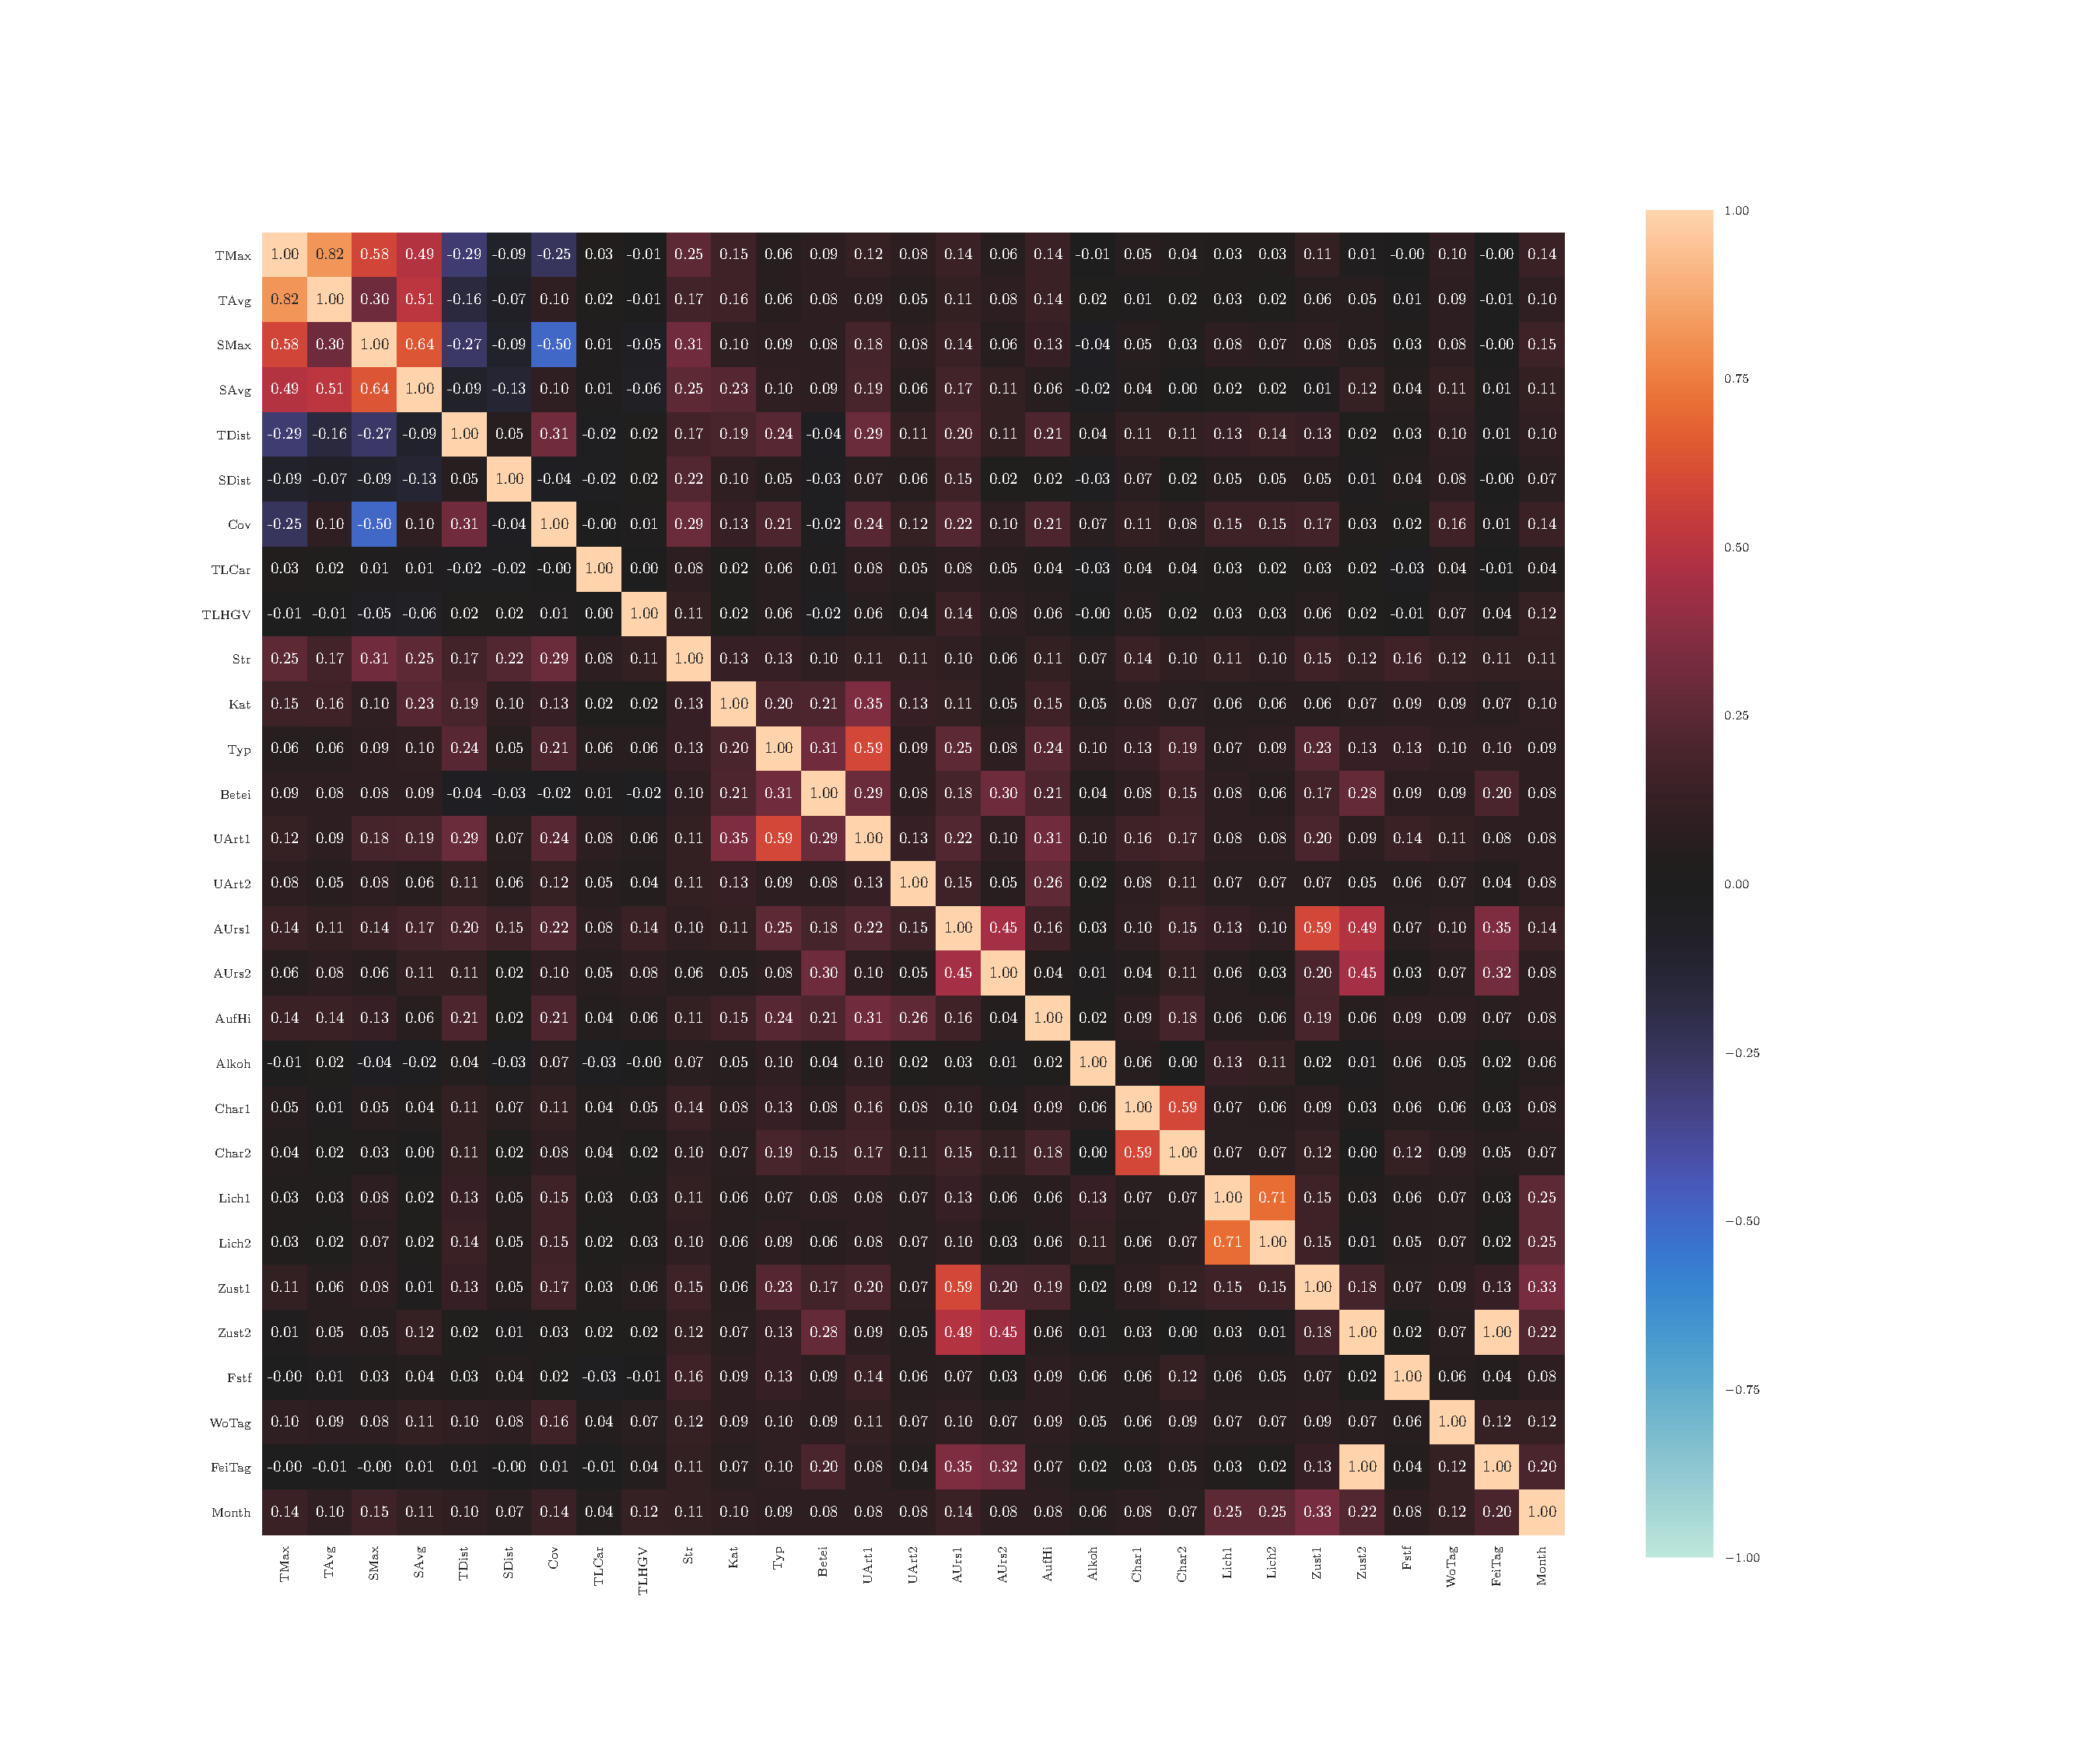
\includegraphics[width=1.4\textwidth, trim=0cm 2.5cm 6cm 3cm]{CorrAnalysis/data/BAYSIS/02_matched/plots/baysis_matched_corr_cramers}%
	}
	\caption{Correlation matrix for congestion-accident matched data calculated with $V$, $\eta$, $\tau$, $r_{pq}$, $r$}
	\label{img:correlation_matrix_matched_cramers}
\end{figure}

% --------------------------
% -------- Strasse ---------
% --------------------------
\centerheading{Street}
This section analyzes the correlated relations of the accident variable \textit{Str}. The correlations of \textit{Str} - \textit{TDist} and \textit{Str} - \textit{SDist} produces a $p$-value above the $\alpha$-level in the Kruskal-Wallis test. The null hypothesis therefore can't be rejected for these relations and there are no significant groups to identify.

The Kruskal-Wallis test of \textit{Str} - \textit{TMax} produces a $p$-value below 0.0001, which is below the $\alpha$-level. The null hypothesis can therefore be rejected, which means that there is a significant difference between the groups of \textit{Str}. To identify the significant groups the pairwise Wilcoxon $T$-test of \textit{Str}-\textit{TMax} produces \cref{tbl:wilcoxon_baysis_matched_Str_TMax}. 
\begin{table}[ht!]
	\tiny
	\setlength{\tabcolsep}{4pt}
	\centering
	\begin{tabular}{rrrrrrrrrrrrrrrrr}
		\toprule
				& A3 & A6 & A9 & A70 & A96 & A7 & A73 & A99 & A92 & A93 & A94 & A72 & A995 & A95 & A71 & A45 \\ 
		\midrule
		% A6 		& 0.00 &  &  &  &  &  &  &  &  &  &  &  &  &  &  &  \\ 
		A9 		& \red{0.01} & 1.00 &  &  &  &  &  &  &  &  &  &  &  &  &  &  \\ 
		A70 	& \red{0.03} & 1.00 & 1.00 &  &  &  &  &  &  &  &  &  &  &  &  &  \\ 
		A96 	& \red{0.00} & 1.00 & 0.27 & 1.00 &  &  &  &  &  &  &  &  &  &  &  &  \\ 
		A7 		& \red{0.00} & 1.00 & 1.00 & 1.00 & 1.00 &  &  &  &  &  &  &  &  &  &  &  \\ 
		A73 	& \red{0.00} & 1.00 & 0.31 & 1.00 & 1.00 & 1.00 &  &  &  &  &  &  &  &  &  &  \\ 
		% A99 	& 1.00 & 1.00 & 1.00 & 1.00 & 0.50 & 1.00 & 0.59 &  &  &  &  &  &  &  &  &  \\ 
		A92 	& \red{0.00} & 1.00 & 0.16 & 1.00 & 1.00 & 1.00 & 1.00 & 0.22 &  &  &  &  &  &  &  &  \\ 
		% A93 	& 1.00 & 1.00 & 1.00 & 1.00 & 1.00 & 1.00 & 1.00 & 1.00 & 1.00 &  &  &  &  &  &  &  \\ 
		A94 	& \red{0.01} & 1.00 & 1.00 & 1.00 & 1.00 & 1.00 & 1.00 & 1.00 & 1.00 & 1.00 &  &  &  &  &  &  \\ 
		% A72 	& 1.00 & 1.00 & 1.00 & 1.00 & 1.00 & 1.00 & 1.00 & 1.00 & 1.00 & 1.00 & 1.00 &  &  &  &  &  \\ 
		% A995 	& 1.00 & 1.00 & 1.00 & 1.00 & 1.00 & 1.00 & 1.00 & 1.00 & 1.00 & 1.00 & 1.00 & 1.00 &  &  &  &  \\ 
		% A95 	& 1.00 & 1.00 & 1.00 & 1.00 & 1.00 & 1.00 & 1.00 & 1.00 & 1.00 & 1.00 & 1.00 & 1.00 & 1.00 &  &  &  \\ 
		% A71 	& 1.00 & 1.00 & 1.00 & 1.00 & 1.00 & 1.00 & 1.00 & 1.00 & 1.00 & 1.00 & 1.00 & 1.00 & 1.00 & 1.00 &  &  \\ 
		% A45 	& 1.00 & 1.00 & 1.00 & 1.00 & 1.00 & 1.00 & 1.00 & 1.00 & 1.00 & 1.00 & 1.00 & 1.00 & 1.00 & 1.00 & 1.00 &  \\ 
		% A980 	& 1.00 & 1.00 & 1.00 & 1.00 & 1.00 & 1.00 & 1.00 & 1.00 & 1.00 & 1.00 & 1.00 & 1.00 & 1.00 & 1.00 & 1.00 & 1.00 \\ 
		\bottomrule
	\end{tabular}
	\caption{Pairwise Wilcoxon $T$-test for \textit{Street} and \textit{Maximal Temporal Extent}}
	\label{tbl:wilcoxon_baysis_matched_Str_TMax}
\end{table}
It shows that the groups A6, A9, A7, A70, A73, A92, A94 and A96 differ from group A3, but is no distinctive general trend.
\begin{table}[ht!]
	\tiny
	\centering
	\begin{tabular}{c|c|c|c|c|c|c|c}
		\toprule
		Group & $n$ & $\bar{x}$ & $\sigma$ & $\tilde{x}$ & $min$ & $max$ & $\Delta$ \\ 
		\midrule
		A3  & 559 & 225.76 & 210.36 & 156.00 & 9  & 1323 & 1314 \\ 
		A6  & 127 & 153.05 & 150.42 & 108.00 & 12 & 864  & 852  \\ 
		A9  & 466 & 170.85 & 151.33 & 118.50 & 9  & 1194 & 1185 \\ 
		A70 & 31  & 106.55 & 79.42  & 81.00  & 24 & 369  & 345  \\ 
		A96 & 155 & 118.32 & 81.05  & 108.00 & 12 & 384  & 372  \\ 
		A7  & 130 & 153.37 & 194.10 & 102.00 & 9  & 1341 & 1332 \\ 
		A73 & 129 & 125.95 & 135.01 & 93.00  & 12 & 1323 & 1311 \\ 
		A99 & 116 & 169.09 & 136.72 & 138.00 & 15 & 681  & 666  \\ 
		A92 & 66  & 103.86 & 65.69  & 87.00  & 18 & 354  & 336  \\ 
		A93 & 21  & 163.57 & 155.71 & 111.00 & 36 & 588  & 552  \\ 
		A94 & 37  & 101.59 & 54.60  & 99.00  & 15 & 249  & 234  \\ 
 		\bottomrule
	\end{tabular}
	\caption{Group descriptives of \textit{Street} and \textit{Maximal Temporal Extent}}
	\label{tbl:descriptives_baysis_matched_Str_TMax}
	%\vspace{-8mm}
\end{table}
The descriptives from \cref{tbl:descriptives_baysis_matched_Str_TMax} show that the mean value of A3 is 27\,\% - 57\,\% higher than the means of A6, A7, A9, A70, A73, A92, and A94. It can be interpreted that accidents on the A3 are associated with significantly longer (temporal) jams than on the A6, A9, A7, A70, A73, A92, and A94. The $\sigma$ supports this interpretation of by $\bar{x}$. The descriptives clearly show three ranked groups of short (A94, A93, A92, A70), medium (A99, A73, A7, A96, A9, A6) and long (A3).

The Kruskal-Wallis test of \textit{Str} - \textit{TAvg} produces a $p$-value of 0.0004, which is below the $\alpha$-level. The null hypothesis can therefore be rejected, which means there is a significant difference between the groups of \textit{Str}. To identify the significant groups the pairwise Wilcoxon $T$-test of \textit{Str}-\textit{TAvg} produces \cref{tbl:wilcoxon_baysis_matched_Str_TAvg}. 
\begin{table}[ht!]
	\tiny
	\setlength{\tabcolsep}{4pt}
	\centering
	\begin{tabular}{rrrrrrrrrrrrrrrrr}
		\toprule
				& A3 & A6 & A9 & A70 & A96 & A7 & A73 & A99 & A92 & A93 & A94 & A72 & A995 & A95 & A71 & A45 \\ 
		\midrule
		% A6 	 & 0.84 &  &  &  &  &  &  &  &  &  &  &  &  &  &  &  \\ 
		% A9 	 & 0.36 & 1.00 &  &  &  &  &  &  &  &  &  &  &  &  &  &  \\ 
		% A70	 & 1.00 & 1.00 & 1.00 &  &  &  &  &  &  &  &  &  &  &  &  &  \\ 
		% A96  & 0.10 & 1.00 & 1.00 & 1.00 &  &  &  &  &  &  &  &  &  &  &  &  \\ 
		% A7 	 & 1.00 & 1.00 & 1.00 & 1.00 & 1.00 &  &  &  &  &  &  &  &  &  &  &  \\ 
		A73  & \red{0.00} & 1.00 & 0.51 & 1.00 & 1.00 & 1.00 &  &  &  &  &  &  &  &  &  &  \\ 
		A99  & \red{0.02} & 1.00 & 1.00 & 1.00 & 1.00 & 1.00 & 1.00 &  &  &  &  &  &  &  &  &  \\ 
		% A92  & 0.26 & 1.00 & 1.00 & 1.00 & 1.00 & 1.00 & 1.00 & 1.00 &  &  &  &  &  &  &  &  \\ 
		% A93  & 1.00 & 1.00 & 1.00 & 1.00 & 1.00 & 1.00 & 1.00 & 1.00 & 1.00 &  &  &  &  &  &  &  \\ 
		% A94  & 0.28 & 1.00 & 1.00 & 1.00 & 1.00 & 1.00 & 1.00 & 1.00 & 1.00 & 1.00 &  &  &  &  &  &  \\ 
		% A72  & 1.00 & 1.00 & 1.00 & 1.00 & 1.00 & 1.00 & 1.00 & 1.00 & 1.00 & 1.00 & 1.00 &  &  &  &  &  \\ 
		% A995 & 1.00 & 1.00 & 1.00 & 1.00 & 1.00 & 1.00 & 1.00 & 1.00 & 1.00 & 1.00 & 1.00 & 1.00 &  &  &  &  \\ 
		% A95  & 1.00 & 1.00 & 1.00 & 1.00 & 1.00 & 1.00 & 1.00 & 1.00 & 1.00 & 1.00 & 1.00 & 1.00 & 1.00 &  &  &  \\ 
		% A71	 & 1.00 & 1.00 & 1.00 & 1.00 & 1.00 & 1.00 & 1.00 & 1.00 & 1.00 & 1.00 & 1.00 & 1.00 & 1.00 & 1.00 &  &  \\ 
		% A45  & 1.00 & 1.00 & 1.00 & 1.00 & 1.00 & 1.00 & 1.00 & 1.00 & 1.00 & 1.00 & 1.00 & 1.00 & 1.00 & 1.00 & 1.00 &  \\ 
		% A980 & 1.00 & 1.00 & 1.00 & 1.00 & 1.00 & 1.00 & 1.00 & 1.00 & 1.00 & 1.00 & 1.00 & 1.00 & 1.00 & 1.00 & 1.00 & 1.00 \\
		\bottomrule
	\end{tabular}
	\caption{Pairwise Wilcoxon $T$-test for \textit{Street} and \textit{Average Temporal Extent}}
	\label{tbl:wilcoxon_baysis_matched_Str_TAvg}
\end{table}
The table shows, that the groups A73 and A99 differ from group A3, but there is no distinctive general trend.
\begin{table}[ht!]
	\tiny
	\centering
	\begin{tabular}{c|c|c|c|c|c|c|c}
		\toprule
		Group & $n$ & $\bar{x}$ & $\sigma$ & $\tilde{x}$ & $min$ & $max$ & $\Delta$ \\  
		\midrule
		A3  & 559 & 89.66 & 98.94  & 65.00 & 4  & 1260 & 1256 \\ 
		A6  & 127 & 69.94 & 65.86  & 56.00 & 3  & 376  & 373  \\ 
		A9  & 466 & 72.92 & 64.55  & 54.00 & 4  & 575  & 571  \\ 
		A70 & 31  & 50.10 & 23.99  & 49.00 & 10 & 99   & 89   \\ 
		A96 & 155 & 61.37 & 44.31  & 52.50 & 5  & 247  & 242  \\ 
		A7  & 130 & 86.55 & 146.82 & 59.50 & 6  & 1326 & 1320 \\ 
		A73 & 129 & 54.78 & 42.48  & 45.00 & 6  & 274  & 268  \\ 
		A99 & 116 & 58.97 & 48.35  & 47.50 & 4  & 295  & 291  \\ 
		A92 & 66  & 55.24 & 36.43  & 51.50 & 8  & 235  & 227  \\ 
		A93 & 21  & 82.33 & 91.10  & 48.00 & 7  & 343  & 336  \\ 
		A94 & 37  & 49.86 & 31.63  & 44.00 & 14 & 145  & 131  \\ 
		\bottomrule
	\end{tabular}
	\caption{Group descriptives for \textit{Street} and \textit{Average Temporal Extent}}
	\label{tbl:descriptives_baysis_matched_Str_TAvg}
	%\vspace{-8mm}
\end{table}
The descriptives from \cref{tbl:descriptives_baysis_matched_Str_TAvg} show that the mean value of A3 is about $\frac{1}{3}$ higher than the means of A73 and A96. We can interpret that accidents on the A3 are associated with significantly longer (temporal) jams than on A73 and A96. The descriptives also show general increase of $\bar{x}$ and $\sigma$ around 35\,\% between the roads A94, A92, A73 and A70 to A3, A6, A7 and A9.

The Kruskal-Wallis test of \textit{Str} - \textit{SMax} produces a $p$-value below 0.0001, which is below the $\alpha$-level. The null hypothesis can therefore be rejected, which means there is a significant difference between the groups of \textit{Str}. To identify the significant groups, a pairwise Wilcoxon $T$-test for \textit{Str} - \textit{SMax} is run, which produces \cref{tbl:wilcoxon_baysis_matched_Str_SMax}.
\begin{table}[ht!]
	\tiny
	\setlength{\tabcolsep}{4pt}
	\centering
	\begin{tabular}{rrrrrrrrrrrrrrrrr}
		\toprule
				& A3   & A6   & A9   & A70  & A96  & A7   & A73   & A99 & A92 & A93 & A94 & A72 & A995 & A95 & A71 & A45 \\ 
		\midrule
		% A6 		& 0.40 &  &  &  &  &  &  &  &  &  &  &  &  &  &  &  \\ 
		A9 		& \red{0.00} & 1.00 &  &  &  &  &  &  &  &  &  &  &  &  &  &  \\ 
		A70 	& \red{0.00} & 0.83 & 0.54 &  &  &  &  &  &  &  &  &  &  &  &  &  \\ 
		A96 	& \red{0.00} & 1.00 & 0.14 & 1.00 &  &  &  &  &  &  &  &  &  &  &  &  \\ 
		A7 		& \red{0.00} & 1.00 & 1.00 & 1.00 & 1.00 &  &  &  &  &  &  &  &  &  &  &  \\ 
		A73 	& \red{0.00} & \red{0.00} & \red{0.00} & 1.00 & 1.00 & 0.59 &  &  &  &  &  &  &  &  &  &  \\ 
		A99 	& 1.00 & 1.00 & 1.00 & 0.80 & 0.31 & 1.00 & \red{0.00} &  &  &  &  &  &  &  &  &  \\ 
		A92 	& \red{0.00} & \red{0.00} & \red{0.00} & 1.00 & 1.00 & 1.00 & 1.00 & \red{0.00} &  &  &  &  &  &  &  &  \\ 
		A93 	& \red{0.03} & 1.00 & 1.00 & 1.00 & 1.00 & 1.00 & 1.00 & 1.00 & 1.00 &  &  &  &  &  &  &  \\ 
		A94 	& \red{0.00} & 0.11 & \red{0.03} & 1.00 & 1.00 & 1.00 & 1.00 & 0.09 & 1.00 & 1.00 &  &  &  &  &  &  \\ 
		% A72 	& 1.00 & 1.00 & 1.00 & 1.00 & 1.00 & 1.00 & 1.00 & 1.00 & 1.00 & 1.00 & 1.00 &  &  &  &  &  \\ 
		% A995 	& 1.00 & 1.00 & 1.00 & 1.00 & 1.00 & 1.00 & 1.00 & 1.00 & 1.00 & 1.00 & 1.00 & 1.00 &  &  &  &  \\ 
		% A95 	& 1.00 & 1.00 & 1.00 & 1.00 & 1.00 & 1.00 & 1.00 & 1.00 & 1.00 & 1.00 & 1.00 & 1.00 & 1.00 &  &  &  \\ 
		% A71 	& 1.00 & 1.00 & 1.00 & 1.00 & 1.00 & 1.00 & 1.00 & 1.00 & 1.00 & 1.00 & 1.00 & 1.00 & 1.00 & 1.00 &  &  \\ 
		% A45 	& 1.00 & 1.00 & 1.00 & 1.00 & 1.00 & 1.00 & 1.00 & 1.00 & 1.00 & 1.00 & 1.00 & 1.00 & 1.00 & 1.00 & 1.00 &  \\ 
		% A980 	& 1.00 & 1.00 & 1.00 & 1.00 & 1.00 & 1.00 & 1.00 & 1.00 & 1.00 & 1.00 & 1.00 & 1.00 & 1.00 & 1.00 & 1.00 & 1.00 \\ 
		\bottomrule
	\end{tabular}
	\caption{Pairwise Wilcoxon $T$-test for \textit{Street} and \textit{Maximal Spatial Extent}}
	\label{tbl:wilcoxon_baysis_matched_Str_SMax}
\end{table}
\cref{tbl:wilcoxon_baysis_matched_Str_SMax} shows, that the groups A7, A9, A70, A73, A92, A94 and A96 differ from group A3. The groups A73 and A92 further differ from group A6 and A9. The group A99 differs from group A73 and group A92 differs from A99, but there is no distinctive general trend.
\begin{table}[ht!]
	\tiny
	\centering
	\begin{tabular}{c|c|c|c|c|c|c|c}
		\toprule
		Group & $n$ & $\bar{x}$ & $\sigma$ & $\tilde{x}$ & $min$ & $max$ & $\Delta$ \\  
		\midrule
		A3  & 559 & 13874.96 & 10064.51 & 11014.00 & 1084 & 46328 & 45244 \\ 
		A6  & 127 & 11067.98 & 8428.07  & 8634.00  & 965  & 43156 & 42191 \\ 
		A9  & 466 & 10680.48 & 7724.45  & 8977.50  & 832  & 49765 & 48933 \\ 
		A70 & 31  & 6676.39  & 3640.24  & 6136.00  & 1841 & 13058 & 11217 \\ 
		A96 & 155 & 8551.75  & 6431.18  & 6238.00  & 971  & 27965 & 26994 \\ 
		A7  & 130 & 9018.27  & 7293.14  & 7051.50  & 1108 & 43244 & 42136 \\ 
		A73 & 129 & 6502.88  & 5033.20  & 5327.00  & 1036 & 33764 & 32728 \\ 
		A99 & 116 & 13244.02 & 11313.27 & 9439.50  & 1280 & 48278 & 46998 \\ 
		A92 & 66  & 6186.80  & 4000.10  & 4936.50  & 1176 & 23291 & 22115 \\ 
		A93 & 21  & 6765.00  & 4403.32  & 5323.00  & 1244 & 16922 & 15678 \\ 
		A94 & 37  & 6220.38  & 3984.46  & 5768.00  & 1167 & 15550 & 14383 \\ 
		\bottomrule
	\end{tabular}
	\caption{Group descriptives of \textit{Street} and \textit{Maximal Spatial Extent}}
	\label{tbl:descriptives_baysis_matched_Str_SMax}
	%\vspace{-8mm}
\end{table}
The descriptives from \cref{tbl:descriptives_baysis_matched_Str_SMax} show that the mean of A3 is 44\,\% - 66\,\% higher than the means of A7, A9, A70, A73, A92, A94 and A96. It also shows that the groups A6, A9 and A99 have a up to 50\,\% higher mean than the groups A73 and A92. We can interpret that accidents on the A3, A6, A9 and A99 are associated with significantly longer (spatial) jams than on A7, A73, A92, A94 and A96. Based on the $\bar{x}$ and $\sigma$ the roads can be separated into three groups of short (A94, A93, A92, A73 and A70), medium (A96 and A7) and long (A3, A6, A9 and A99).

The Kruskal-Wallis test of \textit{Str} - \textit{SAvg} produces a $p$-value of 0.0027, which is below $\alpha=.05$. The null hypothesis can therefore be rejected, which means there is a significant difference between the groups of \textit{Str}. To identify the significant groups, a pairwise Wilcoxon $T$-test for \textit{Str} - \textit{SAvg} is run, which produces \cref{tbl:wilcoxon_baysis_matched_Str_SAvg}.
\begin{table}[ht!]
	\tiny
	\setlength{\tabcolsep}{4pt}
	\centering
	\begin{tabular}{rrrrrrrrrrrrrrrrr}
		\toprule
	 		 & A3 & A6 & A9 & A70 & A96 & A7 & A73 & A99 & A92 & A93 & A94 & A72 & A995 & A95 & A71 & A45 \\ 
		\midrule
		% A6   & 1.00 &  &  &  &  &  &  &  &  &  &  &  &  &  &  &  \\ 
	  	% A9   & 1.00 & 1.00 &  &  &  &  &  &  &  &  &  &  &  &  &  &  \\ 
	  	A70  & \red{0.05} & 0.83 & 0.71 &  &  &  &  &  &  &  &  &  &  &  &  &  \\ 
	  	A96  & \red{0.05} & 1.00 & 1.00 & 1.00 &  &  &  &  &  &  &  &  &  &  &  &  \\ 
	  	% A7   & 1.00 & 1.00 & 1.00 & 1.00 & 1.00 &  &  &  &  &  &  &  &  &  &  &  \\ 
	  	A73  & \red{0.00} & \red{0.00} & \red{0.00} & 1.00 & \red{0.00} & \red{0.00} &  &  &  &  &  &  &  &  &  &  \\ 
	  	A99  & \red{0.00} & 1.00 & 0.06 & 1.00 & 1.00 & 1.00 & 0.51 &  &  &  &  &  &  &  &  &  \\ 
	  	A92  & \red{0.00} & 0.61 & \red{0.03} & 1.00 & 1.00 & 1.00 & 1.00 & 1.00 &  &  &  &  &  &  &  &  \\ 
	  	A93  & \red{0.03} & 0.46 & 0.16 & 1.00 & 1.00 & 1.00 & 1.00 & 1.00 & 1.00 &  &  &  &  &  &  &  \\ 
	  	A94  & \red{0.00} & 0.07 & 0.01 & 1.00 & 0.36 & 0.31 & 1.00 & 1.00 & 1.00 & 1.00 &  &  &  &  &  &  \\ 
	  	% A72  & 1.00 & 1.00 & 1.00 & 1.00 & 1.00 & 1.00 & 1.00 & 1.00 & 1.00 & 1.00 & 1.00 &  &  &  &  &  \\ 
	  	% A995 & 1.00 & 1.00 & 1.00 & 1.00 & 1.00 & 1.00 & 1.00 & 1.00 & 1.00 & 1.00 & 1.00 & 1.00 &  &  &  &  \\ 
	  	% A95  & 1.00 & 1.00 & 1.00 & 1.00 & 1.00 & 1.00 & 1.00 & 1.00 & 1.00 & 1.00 & 1.00 & 1.00 & 1.00 &  &  &  \\ 
	  	% A71  & 1.00 & 1.00 & 1.00 & 1.00 & 1.00 & 1.00 & 1.00 & 1.00 & 1.00 & 1.00 & 1.00 & 1.00 & 1.00 & 1.00 &  &  \\ 
	  	% A45  & 1.00 & 1.00 & 1.00 & 1.00 & 1.00 & 1.00 & 1.00 & 1.00 & 1.00 & 1.00 & 1.00 & 1.00 & 1.00 & 1.00 & 1.00 &  \\ 
	  	% A980 & 1.00 & 1.00 & 1.00 & 1.00 & 1.00 & 1.00 & 1.00 & 1.00 & 1.00 & 1.00 & 1.00 & 1.00 & 1.00 & 1.00 & 1.00 & 1.00 \\ 
		\bottomrule
	\end{tabular}
	\caption{Pairwise Wilcoxon $T$-test for \textit{Street} and \textit{Average Spatial Extent}}
	\label{tbl:wilcoxon_baysis_matched_Str_SAvg}
\end{table}
\cref{tbl:wilcoxon_baysis_matched_Str_SAvg} shows, that the groups A70, A73, A92, A93, A94, A96 and A99 differ from group A3. The groups A73, A94 further differ from group A6 as well as A73, A99, A92 and A94 from group A9, but there is no distinctive general trend.
\begin{table}[ht!]
	\tiny
	\centering
	\begin{tabular}{c|c|c|c|c|c|c|c}
	  	\toprule
	 	Group & $n$ & $\bar{x}$ & $\sigma$ & $\tilde{x}$ & $min$ & $max$ & $\Delta$ \\  
	  	\midrule
		A3  & 559 & 4537.56 & 2735.62 & 3986.00 & 135  & 17805 & 17670 \\ 
	  	A6  & 127 & 4361.50 & 3042.71 & 3235.00 & 458  & 16851 & 16393 \\ 
	  	A9  & 466 & 4187.15 & 2569.83 & 3700.50 & 393  & 15132 & 14739 \\ 
	  	A70 & 31  & 3010.45 & 2067.63 & 1974.00 & 1008 & 9937  & 8929 \\ 
	  	A96 & 155 & 3678.39 & 2172.99 & 3299.00 & 387  & 10182 & 9795 \\ 
	  	A7  & 130 & 4141.68 & 3026.58 & 3537.50 & 643  & 16571 & 15928 \\ 
	  	A73 & 129 & 2683.97 & 1981.91 & 2232.00 & 544  & 11832 & 11288 \\ 
	  	A99 & 116 & 3240.97 & 1878.87 & 2978.00 & 583  & 8426  & 7843 \\ 
	  	A92 & 66  & 2926.15 & 1521.59 & 2931.50 & 455  & 8970  & 8515 \\ 
	  	A93 & 21  & 2525.43 & 1443.21 & 2338.00 & 664  & 6779  & 6115 \\ 
	  	A94 & 37  & 2691.68 & 2023.38 & 2307.00 & 358  & 10393 & 10035 \\ 
	   	\bottomrule
	\end{tabular}
	\caption{Group descriptives of \textit{Street} and \textit{Average Spatial Extent}}
	\label{tbl:descriptives_baysis_matched_Str_SAvg}
	%\vspace{-8mm}
\end{table}
The descriptives from \cref{tbl:descriptives_baysis_matched_Str_SAvg} show that the mean of A3 is 45\,\% - 55\,\% higher the means of A70, A73, A92, A93, A94, A96 and A99. It also shows that the means of the groups A6, A9 and A99 is about 30\,\% higher mean than the groups A73 and A94. We can interpret that accidents on the A3, A6, A9 and A99 lead are associated with significantly longer (spatial) jams than on A70, A73, A92, A93, A94, A96 and A99. The groups can be separated into two groups based on $\bar{x}$ and $\sigma$. A3, A6, A9 and A7 tend to have longer (spatial) longer jams when A70, A96, A73, A99, A92, A93 and A94 tend to have shorter (spatial) jams.

The Kruskal-Wallis test of \textit{Str} - \textit{Cov} produces a $p$-value of 0.0018, which is below the $\alpha$-level. The null hypothesis can therefore be rejected, which means there is a significant difference between the groups of \textit{Str}. To identify the significant groups, a pairwise Wilcoxon $T$-test for \textit{Str} - \textit{Cov} is run, which produces \cref{tbl:wilcoxon_baysis_matched_Str_Cov}. 
\begin{table}[ht!]
	\tiny
	\setlength{\tabcolsep}{4pt}
	\centering
	\begin{tabular}{rrrrrrrrrrrrrrrrr}
	  	\toprule
				& A3   & A6   & A9   & A70  & A96  & A7   & A73 & A99 & A92 & A93 & A94 & A72 & A995 & A95 & A71 & A45 \\ 
	  	\midrule
		A6 		& \red{0.05} &  &  &  &  &  &  &  &  &  &  &  &  &  &  &  \\ 
	  	A9 		& \red{0.00} & 1.00 &  &  &  &  &  &  &  &  &  &  &  &  &  &  \\ 
	  	% A70 	& 1.00 & 1.00 & 1.00 &  &  &  &  &  &  &  &  &  &  &  &  &  \\ 
	  	A96 	& \red{0.00} & 1.00 & \red{0.00} & 1.00 &  &  &  &  &  &  &  &  &  &  &  &  \\ 
	  	A7 		& \red{0.00} & 1.00 & \red{0.01} & 1.00 & 1.00 &  &  &  &  &  &  &  &  &  &  &  \\ 
	  	A73 	& \red{0.04} & 1.00 & 1.00 & 1.00 & 1.00 & 1.00 &  &  &  &  &  &  &  &  &  &  \\ 
	  	A99 	& 0.88 & \red{0.00} & \red{0.00} & 0.09 & \red{0.00} & \red{0.00} & \red{0.00} &  &  &  &  &  &  &  &  &  \\ 
	  	A92 	& \red{0.00} & 1.00 & 0.12 & 1.00 & 1.00 & 1.00 & 1.00 & \red{0.00} &  &  &  &  &  &  &  &  \\ 
	  	% A93 	& 1.00 & 1.00 & 1.00 & 1.00 & 1.00 & 1.00 & 1.00 & 1.00 & 1.00 &  &  &  &  &  &  &  \\ 
	  	% A94 	& 1.00 & 1.00 & 1.00 & 1.00 & 1.00 & 1.00 & 1.00 & 0.13 & 1.00 & 1.00 &  &  &  &  &  &  \\ 
	  	% A72 	& 1.00 & 1.00 & 1.00 & 1.00 & 1.00 & 1.00 & 1.00 & 1.00 & 1.00 & 1.00 & 1.00 &  &  &  &  &  \\ 
	  	% A995 	& 1.00 & 1.00 & 1.00 & 1.00 & 1.00 & 1.00 & 1.00 & 1.00 & 1.00 & 1.00 & 1.00 & 1.00 &  &  &  &  \\ 
	  	% A95 	& 1.00 & 1.00 & 1.00 & 1.00 & 1.00 & 1.00 & 1.00 & 1.00 & 1.00 & 1.00 & 1.00 & 1.00 & 1.00 &  &  &  \\ 
	  	% A71 	& 1.00 & 1.00 & 1.00 & 1.00 & 1.00 & 1.00 & 1.00 & 1.00 & 1.00 & 1.00 & 1.00 & 1.00 & 1.00 & 1.00 &  &  \\ 
	  	% A45 	& 1.00 & 1.00 & 1.00 & 1.00 & 1.00 & 1.00 & 1.00 & 1.00 & 1.00 & 1.00 & 1.00 & 1.00 & 1.00 & 1.00 & 1.00 &  \\ 
	  	% A980 	& 1.00 & 1.00 & 1.00 & 1.00 & 1.00 & 1.00 & 1.00 & 1.00 & 1.00 & 1.00 & 1.00 & 1.00 & 1.00 & 1.00 & 1.00 & 1.00 \\ 
	   	\bottomrule
	\end{tabular}
	\caption{Pairwise Wilcoxon $T$-test for \textit{Street} and \textit{Coverage}}
	\label{tbl:wilcoxon_baysis_matched_Str_Cov}
\end{table}
\cref{tbl:wilcoxon_baysis_matched_Str_SAvg} shows, that the groups A6, A7, A9, A73, A92 and A96 differ from group A3. The group A99 differs from group A6 and groups A96, AA7, A99, A92 differ from group A9. The group A99 also differs from the groups A70, A96, A7 and A73, but there is no distinctive general trend. 
\begin{table}[ht!]
	\tiny
	\centering
	\begin{tabular}{c|c|c|c|c|c|c|c}
	  	\toprule
	 	Group & $n$ & $\bar{x}$ & $\sigma$ & $\tilde{x}$ & $min$ & $max$ & $\Delta$ \\   
	  	\midrule
		A3  & 559 & 38.44 & 19.04 & 36.00 & 2  & 100 & 98 \\ 
	  	A6  & 127 & 46.99 & 24.06 & 44.00 & 9  & 100 & 91 \\ 
	  	A9  & 466 & 43.93 & 18.49 & 41.00 & 6  & 100 & 94 \\ 
	  	A70 & 31  & 50.29 & 25.00 & 44.00 & 9  & 92  & 83 \\ 
	  	A96 & 155 & 51.94 & 21.38 & 54.00 & 2  & 100 & 98 \\ 
	  	A7  & 130 & 53.46 & 24.19 & 54.00 & 6  & 100 & 94 \\ 
	  	A73 & 129 & 46.49 & 22.88 & 42.00 & 7  & 100 & 93 \\ 
	  	A99 & 116 & 33.21 & 18.03 & 31.00 & 5  & 85  & 80 \\ 
	  	A92 & 66  & 53.15 & 21.80 & 52.50 & 14 & 98  & 84 \\ 
	  	A93 & 21  & 40.81 & 17.72 & 37.00 & 13 & 70  & 57 \\ 
	  	A94 & 37  & 47.76 & 23.69 & 44.00 & 11 & 88  & 77 \\ 	
	  	\bottomrule
	\end{tabular}
	\caption{Group descriptives of \textit{Street} and \textit{Coverage}}
	\label{tbl:descriptives_baysis_matched_Str_Cov}
	%\vspace{-8mm}
\end{table}
The descriptives from \cref{tbl:descriptives_baysis_matched_Str_Cov} show that the mean of A3 is 20\,\% - 30\,\% lower than the means of A6, A7, A9, A73, A92 and A96. It also shows that the mean of A6 is about $\frac{1}{3}$ higher than the mean of A99. We can interpret that accidents on the A3, A99 are associated with significantly less denser jams than on A6, A7, A9, A73, A70, A92 and A96.

% ----------------------
% -------- Kat ---------
% ----------------------
\centerheading{Kat}
\label{ana:baysis_global_Kat}
This section analyzes the correlated relations of the accident variable \textit{Kat}. The encoding and description of the variable \textit{Typ} is shown in \cref{tbl:baysis_dataset_Typ}. The Kruskal-Wallis rank sum test of \textit{Kat}-\textit{SAvg} produces a $p$-value above $\alpha$. The null hypothesis can't be rejected and there is no significant difference between the groups of \textit{Kat} in this relation.

The Kruskal-Wallis test of \textit{Kat}-\textit{TMax} produces a $p$-value of 0.0068, which is below $\alpha=.05$. The null hypothesis can therefore be rejected, which means there is a significant difference between the groups of \textit{Kat}. To identify the significant groups, a pairwise Wilcoxon $T$-test for \textit{Kat}-\textit{TMax} is run, which produces \cref{tbl:wilcoxon_baysis_matched_Kat_TMax}.
\begin{table}[ht]
	\tiny
	\centering
	\begin{tabular}{rrrr}
	  	\toprule
	 	& 1 & 2 & 3 \\ 
	  	\midrule
		2 & \red{0.00} &  &  \\ 
	  	3 & \red{0.00} & \red{0.01} &  \\ 
	  	7 & \red{0.00} & \red{0.02} & 0.78 \\ 
	   	\bottomrule
	\end{tabular}
	\caption{Pairwise Wilcoxon $T$-test for \textit{Kat} and \textit{Maximal Temporal Extent}}
	\label{tbl:wilcoxon_baysis_matched_Kat_TMax}
\end{table}
\cref{tbl:wilcoxon_baysis_matched_Kat_TMax} shows that all groups, besides of group 7 to group 3, have significant differences. 
\begin{table}[ht]
	\tiny
	\centering
	\begin{tabular}{c|c|c|c|c|c|c|c}
		\toprule
		Group & $n$ & $\bar{x}$ & $\sigma$ & $\tilde{x}$ & $min$ & $max$ & $\Delta$ \\   
	  	\midrule
		1 & 36  & 317.67 & 215.10 & 279 & 27 & 987  & 960 \\ 
	  	2 & 216 & 189.03 & 164.93 & 135 & 9  & 1257 & 1248 \\ 
	  	3 & 881 & 155.26 & 141.87 & 111 & 9  & 1323 & 1314 \\ 
	  	7 & 718 & 179.35 & 192.33 & 117 & 9  & 1341 & 1332 \\ 
	   	\bottomrule
	\end{tabular}
	\caption{Group descriptives of \textit{Kat} and \textit{Maximal Temporal Extent}}
	\label{tbl:descriptives_baysis_matched_Kat_TMax}
	%\vspace{-8mm}
\end{table}
% 189+155+179 / 3 = 174
% diff 317,174 = 143
% mean diff 189,155,179 = 29
The descriptives from \cref{tbl:descriptives_baysis_matched_Kat_TMax} present increasing means from lightly injured to deathly accident. We can interpret that the maximal temporal jam length  increases with the gravity of the accident. Also the difference of group 1 to group 2, 3 and 7 is quite substantial, which means that the accidents with deaths are associated with 143\,min longer jams, than others. The group of accidents with property damage does significantly differ from the others, but does not fit into the trend. A comparisons of means puts the property damage group in-between of accidents with slightly and heavily injured. The groups 2, 3 and 7 differ by 29\,min on average.

The Kruskal-Wallis test of \textit{Kat}-\textit{TAvg} produces a $p$-value of 0.0005, which is below $\alpha$. The null hypothesis can therefore be rejected, which means there is a significant difference between the groups of \textit{Kat}. To identify the significant groups, a pairwise Wilcoxon $T$-test for \textit{Kat}-\textit{TAvg} is run, which produces \cref{tbl:wilcoxon_baysis_matched_Kat_TAvg}.
\begin{table}[ht]
	\tiny
	\centering
	\begin{tabular}{rrrr}
	  	\toprule
	 	& 1 & 2 & 3 \\ 
	  	\midrule
		2 & \red{0.00} &  &  \\ 
	  	3 & \red{0.00} & \red{0.00} &  \\ 
	  	7 & \red{0.00} & \red{0.00} & \red{0.05} \\ 
	   	\bottomrule
	\end{tabular}
	\caption{Pairwise Wilcoxon $T$-test for \textit{Kat} and \textit{Average Temporal Extent}}
	\label{tbl:wilcoxon_baysis_matched_Kat_TAvg}
\end{table}
\cref{tbl:wilcoxon_baysis_matched_Kat_TAvg} shows that all groups have significant differences. The descriptives from \cref{tbl:descriptives_baysis_matched_Kat_TAvg} present increasing means from group 3 to 1.
\begin{table}[ht]
	\tiny
	\centering
	\begin{tabular}{c|c|c|c|c|c|c|c}
	  	\toprule
		Group & $n$ & $\bar{x}$ & $\sigma$ & $\tilde{x}$ & $min$ & $max$ & $\Delta$ \\ 
	  	\midrule
		1 & 36  & 156.06 & 104.55 & 143.00 & 20 & 502  & 482  \\ 
	  	2 & 216 & 88.31  & 79.73  & 66.50  & 7  & 703  & 696  \\ 
	  	3 & 881 & 67.32  & 53.98  & 54.00  & 3  & 469  & 466  \\ 
	  	7 & 718 & 74.08  & 103.32 & 51.00  & 4  & 1326 & 1322 \\ 
	   	\bottomrule
	\end{tabular}
	\caption{Group descriptives of \textit{Kat} and \textit{Average Temporal Extent}}
	\label{tbl:descriptives_baysis_matched_Kat_TAvg}
	%\vspace{-8mm}
\end{table}
% 88+67+74 / 3 = 76
% diff 156,76 = 80
% mean diff 88,67,74 = 10
We can interpret that the average temporal jam length increases with the gravity of the accident. Also the difference of group 1 to group 2, 3 and 7 is quite substantial, which means that the accidents with deaths are associated with 80\,min longer jams than others. The group of accidents with property damage does significantly differ from the others, but does not fit into the trend. A comparisons of means puts the group in-between of accidents with slightly and heavily injured. The groups 2, 3 and 7 differ by 10\,min on average. 

The Kruskal-Wallis test of \textit{Kat}-\textit{TDist} produces a $p$-value below 0.0001, which is way below the $\alpha$-level. The null hypothesis can therefore be rejected, which means there is a significant difference between the groups of \textit{Kat}. To identify the significant groups, a pairwise Wilcoxon $T$-test for \textit{Kat}-\textit{TDist} is run, which produces \cref{tbl:wilcoxon_baysis_matched_Kat_TDist}. 
\begin{table}[ht]
	\tiny
	\centering
	\begin{tabular}{rrrr}
		\toprule
		& 1 & 2 & 3 \\ 
		\midrule
		2 & \red{0.05} &  &  \\ 
		3 & \red{0.00} & \red{0.00} &  \\ 
		7 & \red{0.00} & \red{0.00} & \red{0.00} \\ 
		\bottomrule
	\end{tabular}
	\caption{Pairwise Wilcoxon $T$-test for \textit{Kat} and \textit{Temporal Distance}}
	\label{tbl:wilcoxon_baysis_matched_Kat_TDist}
\end{table}
\cref{tbl:wilcoxon_baysis_matched_Kat_TDist} shows that all groups have significant differences. 
\begin{table}[ht]
	\tiny
	\centering
	\begin{tabular}{c|c|c|c|c|c|c|c}
	  	\toprule
		Group & $n$ & $\bar{x}$ & $\sigma$ & $\tilde{x}$ & $min$ & $max$ & $\Delta$ \\ 
	  	\midrule
		1 & 36  & 10.39 & 7.36 & 10.00 & 0.00 & 22.00 & 22.00 \\ 
	  	2 & 216 & 7.91 & 6.92 & 7.00 & 0.00 & 24.00 & 24.00 \\ 
	  	3 & 881 & 5.81 & 6.82 & 4.00 & 0.00 & 24.00 & 24.00 \\ 
	  	7 & 718 & 4.33 & 6.63 & 0.00 & 0.00 & 24.00 & 24.00 \\ 
	   	\bottomrule
	\end{tabular}
	\caption{Group descriptives of \textit{Kat} and \textit{Temporal Distance}}
	\label{tbl:descriptives_baysis_matched_Kat_TDist}
	%\vspace{-8mm}
\end{table}
The descriptives from \cref{tbl:descriptives_baysis_matched_Kat_TDist} present increasing means from group 4 to 1. We can interpret that the temporal distance from accidents to jams increases with the gravity of the accident.

% ----------------------
% -------- Typ ---------
% ----------------------
\centerheading{Typ}
This section analyzes the correlated relations of the accident variable \textit{Typ}. Groups with an insufficient sample size (see \cref{correlation_uncertainty} are neglected and not considered. The encoding and description of the variable \textit{Typ} is shown in \cref{tbl:baysis_dataset_Typ}. The Kruskal-Wallis rank sum test of \textit{Typ}-\textit{Cov} produces a $p$-value above $\alpha$. The null hypothesis can't be rejected and there is no significant difference between the groups of \textit{Typ} in this relation.

The Kruskal-Wallis rank sum test of \textit{Typ}-\textit{TDist} produces a $p$-value of 0.0005, which is below $\alpha$. The null hypothesis can therefore be rejected, which means there is a significant difference between the groups of \textit{Typ}. To identify the significant groups, a pairwise Wilcoxon $T$-test for \textit{Typ}-\textit{TDist} is run, which produces \cref{tbl:wilcoxon_baysis_matched_Typ_TDist}. 
\begin{table}[ht]
	\tiny
	\centering
	\begin{tabular}{rrrrrr}
		\toprule
		& 1 & 3 & 4 & 5 & 6 \\ 
		\midrule
		3 & \red{0.00} &  &  &  &  \\ 
		4 & 0.54 & \red{0.01} &  &  &  \\ 
		5 & 0.54 & 0.58 & 0.23 &  &  \\ 
		6 & \red{0.00} & \red{0.00} & \red{0.05} & 1.00 &  \\ 
		7 & 1.00 & \red{0.00} & 0.54 & 0.54 & \red{0.00} \\ 
		\bottomrule
	\end{tabular}
	\caption{Pairwise Wilcoxon $T$-test for \textit{Typ} and \textit{Temporal Distance}}
	\label{tbl:wilcoxon_baysis_matched_Typ_TDist}
\end{table}
The $p$-values in \cref{tbl:wilcoxon_baysis_matched_Kat_TDist} show the groups 3 and 6 differ from 1, group 6 and 7 differ from 3 and group 7 differs from 6.
\begin{table}[ht]
	\tiny
	\centering
	\begin{tabular}{c|c|c|c|c|c|c|c}
		\toprule
		Group & $n$ & $\bar{x}$ & $\sigma$ & $\tilde{x}$ & $min$ & $max$ & $\Delta$ \\ 
		\midrule
		1 & 300  & 8.33 & 7.39 & 7 & 0 & 24 & 24 \\ 
		3 & 120  & 2.91 & 5.46 & 0 & 0 & 22 & 22 \\ 
		6 & 1299 & 4.78 & 6.49 & 1 & 0 & 24 & 24 \\ 
		7 & 117  & 8.70 & 8.15 & 7 & 0 & 24 & 24 \\ 
		\bottomrule
	\end{tabular}
	\caption{Group descriptives of \textit{Typ} and \textit{Temporal Distance}}
	\label{tbl:descriptives_baysis_matched_Typ_TDist}
	%\vspace{-8mm}
\end{table}
The descriptives in \cref{tbl:descriptives_baysis_matched_Typ_TDist} reveal that the groups 1 and 7 have a higher $\bar{x}$ than group 3 and 6. We can interpret that temporal distance of \textit{driving} and \textit{other} (average of 12\,min) accidents is substantial higher than for \textit{merging}, \textit{crossing} and \textit{straight traffic} (average of 8\,min) accidents. 

% -----------------------
% -------- UArt ---------
% -----------------------
\centerheading{UArt}
This section analyzes the correlated relations of the accident variable \textit{UArt}. Groups with an insufficient sample size (see \cref{correlation_uncertainty} are neglected and not considered. The encoding and description of the variable \textit{UArt} is shown in \cref{tbl:baysis_dataset_UArt}. The Kruskal-Wallis rank sum test of \textit{UArt}-\textit{SAvg} produces a $p$-value of 0.2081, which is above the $\alpha$-level. The null hypothesis can't be rejected and there is \textit{no} significant difference between the groups of \textit{UArt}. There are no significant groups to identify.

The Kruskal-Wallis test of \textit{UArt}-\textit{TDist} produces a $p$-value of below 0.0001, which is way below $\alpha$. The null hypothesis can therefore be rejected, which means there is a significant difference between the groups of \textit{UArt}. To identify the significant groups, a pairwise Wilcoxon $T$-test for \textit{UArt}-\textit{TDist} is run, which produces \cref{tbl:wilcoxon_baysis_matched_UArt_TDist}. 
\begin{table}[ht]
	\tiny
	\centering
	\begin{tabular}{rrrrrrrrrr}
  		\toprule
		  & 0 & 1 & 2 & 3 & 4 & 5 & 6 & 7 & 8 \\ 
		\midrule
		% 1 & 1.00 &  &  &  &  &  &  &  &  \\ 
		% 2 & 1.00 & 1.00 &  &  &  &  &  &  &  \\ 
		% 3 & 1.00 & 1.00 & 1.00 &  &  &  &  &  &  \\ 
		% 4 & 0.57 & 0.22 & 0.31 & 0.17 &  &  &  &  &  \\ 
		5 & \red{0.04} & 0.17 & \red{0.00} & \red{0.00} & \red{0.01} &  &  &  &  \\ 
		6 & 0.40 & 0.19 & 0.23 & 0.16 & 1.00 & \red{0.01} &  &  &  \\ 
		7 & \red{0.00} & \red{0.00} & \red{0.00} & \red{0.00} & 1.00 & \red{0.00} & 1.00 &  &  \\ 
		8 & \red{0.02} & \red{0.00} & \red{0.00} & \red{0.00} & 1.00 & \red{0.00} & 1.00 & 0.32 &  \\ 
		9 & \red{0.01} & \red{0.00} & \red{0.00} & \red{0.00} & 1.00 & \red{0.00} & 1.00 & 0.50 & 1.00 \\ 
		\bottomrule
	\end{tabular}
	\caption{Pairwise Wilcoxon $T$-test for \textit{UArt} and \textit{Temporal Distance}}
	\label{tbl:wilcoxon_baysis_matched_UArt_TDist}
\end{table}
The $p$-values in \cref{tbl:wilcoxon_baysis_matched_UArt_TDist} show that group 5 differs from 2, 3 and 4. The groups 7, 8 and 9 differ from the groups 0, 1, 2, 3 and 5. The descriptives in \cref{tbl:descriptives_baysis_matched_UArt_TDist} reveal that group 5 has the lowest $\bar{x}$ and $\sigma$ of all groups and the groups 7, 8 and 9 have the highest. This can be interpreted as accident collisions with \textit{turning} and \textit{crossing} vehicles have a close temporal reaction, when jams of accident collisions with \textit{obstacles} or \textit{left/right} nearby vehicles take longer to create (average of 10\,min). The categories describing \textit{starting}, \textit{standing}, \textit{stopping}, \textit{ahead and waiting vehicle} and \textit{vehicle on separate lane in same direction} have an average of 5\,min.
\begin{table}[ht]
	\tiny
	\centering
	\begin{tabular}{c|c|c|c|c|c|c|c}
		\hline
		Group & $n$ & $\bar{x}$ & $\sigma$ & $\tilde{x}$ & $min$ & $max$ & $\Delta$ \\
		\hline
		0 & 63  & 5.30  & 6.83 & 0.00  & 0 & 22 & 22 \\ 
		1 & 86  & 4.44  & 6.58 & 0.00  & 0 & 24 & 24 \\ 
		2 & 831 & 5.05  & 6.53 & 1.00  & 0 & 24 & 24 \\ 
		3 & 447 & 4.53  & 6.30 & 0.00  & 0 & 24 & 24 \\ 
		5 & 90  & 2.44  & 5.48 & 0.00  & 0 & 24 & 24 \\  
		7 & 35  & 12.63 & 8.62 & 14.00 & 0 & 24 & 24 \\ 
		8 & 165 & 8.79  & 7.55 & 8.00  & 0 & 24 & 24 \\ 
		9 & 124 & 9.10  & 7.00 & 9.00  & 0 & 24 & 24 \\ 
		\hline
	\end{tabular}
	\caption{Group descriptives of \textit{UArt} and \textit{Temporal Distance}}
	\label{tbl:descriptives_baysis_matched_UArt_TDist}
	%\vspace{-8mm}
\end{table}

The Kruskal-Wallis test of \textit{UArt}-\textit{Cov} produces a $p$-value of 0.0001, which is below $\alpha$. The null hypothesis can therefore be rejected, which means there is a significant difference between the groups of \textit{UArt}. To identify the significant groups, a pairwise Wilcoxon $T$-test for \textit{UArt}-\textit{Cov} is run, which produces \cref{tbl:wilcoxon_baysis_matched_UArt_Cov}.
\begin{table}[ht]
	\tiny
	\centering
	\begin{tabular}{rrrrrrrrrr}
		\toprule
		  & 0 & 1 & 2 & 3 & 4 & 5 & 6 & 7 & 8 \\ 
		\midrule
		% 1 & 1.00 &  &  &  &  &  &  &  &  \\ 
		% 2 & 1.00 & 1.00 &  &  &  &  &  &  &  \\ 
		% 3 & 1.00 & 1.00 & 1.00 &  &  &  &  &  &  \\ 
		% 4 & 1.00 & 1.00 & 1.00 & 1.00 &  &  &  &  &  \\ 
		5 & 0.41 & 0.10 & \red{0.00} & \red{0.01} & 0.65 &  &  &  &  \\ 
		% 6 & 1.00 & 1.00 & 1.00 & 1.00 & 1.00 & 1.00 &  &  &  \\ 
		7 & 0.30 & 0.36 & 0.12 & \red{0.05} & 1.00 & \red{0.00} & 1.00 &  &  \\ 
		8 & \red{0.01} & \red{0.01} & \red{0.00} & \red{0.00} & 1.00 & \red{0.00} & 1.00 & 1.00 &  \\ 
		9 & \red{0.05} & 0.07 & \red{0.00} & \red{0.00} & 1.00 & \red{0.00} & 1.00 & 1.00 & 1.00 \\ 
		\bottomrule
	\end{tabular}
	\caption{Pairwise Wilcoxon $T$-test for \textit{UArt} and \textit{Coverage}}
	\label{tbl:wilcoxon_baysis_matched_UArt_Cov}
\end{table}
The $p$-values in \cref{tbl:wilcoxon_baysis_matched_UArt_TDist} show that group 5 differs from 2, 3 and group 7 differs from group 3. Further does the group 8 differs from groups 0, 1 ,2 , 3 and 5. Group 9 differs from 2, 3 and 4.
\begin{table}[ht]
	\tiny
	\centering
	\begin{tabular}{c|c|c|c|c|c|c|c}
		\toprule
		Group & $n$ & $\bar{x}$ & $\sigma$ & $\tilde{x}$ & $min$ & $max$ & $\Delta$ \\ 
		\midrule
		0 & 63  & 41.40 & 20.09 & 37.00 & 5  & 96  & 91 \\ 
		1 & 86  & 42.29 & 20.19 & 40.50 & 2  & 96  & 94 \\ 
		2 & 831 & 42.86 & 20.00 & 41.00 & 2  & 100 & 98 \\ 
		3 & 447 & 41.21 & 19.59 & 39.00 & 2  & 98  & 96 \\  
		5 & 90  & 33.81 & 18.18 & 30.00 & 10 & 88  & 78 \\ 
		7 & 35  & 56.31 & 26.88 & 56.00 & 11 & 100 & 89 \\ 
		8 & 165 & 53.96 & 24.35 & 53.00 & 7  & 100 & 93 \\ 
		9 & 124 & 52.44 & 23.26 & 49.00 & 3  & 100 & 97 \\ 
		\bottomrule
	\end{tabular}
	\caption{Group descriptives of \textit{UArt} and \textit{Coverage}}
	\label{tbl:descriptives_baysis_matched_UArt_Cov}
	%\vspace{-8mm}
\end{table}
The descriptives in \cref{tbl:descriptives_baysis_matched_UArt_TDist} reveal that group 5 has the lowest $\bar{x}$ of all groups. The groups 7, 8 and 9 have the highest $\sigma$. This can be interpreted as accident collisions with \textit{turning} and \textit{crossing} vehicles are associated with lesser dense jams, when accident collisions with \textit{obstacles} or \textit{left/right} nearby vehicles are related with 20\,\% denser jams (average of 65\,\%). The categories describing \textit{starting}, \textit{standing}, \textit{stopping}, \textit{ahead and waiting vehicle} and \textit{vehicle on separate lane in same direction} have an average of 41\,\%.

% -----------------------
% -------- AUrs ---------
% -----------------------
\centerheading{AUrs}
This section analyzes the correlated relations of the accident variable \textit{AUrs}. Groups with an insufficient sample size (see \cref{correlation_uncertainty} are neglected and not considered. The encoding and description of the variable \textit{AUrs} is shown in \cref{tbl:baysis_dataset_AUrs}. The variable value of group 0, which occurs in the dataset is undefined by BAYSIS and will be therefore neglected for the interpretation. The Kruskal-Wallis tests of \textit{AUrs}-\textit{SDist} and \textit{AUrs}-\textit{TLHGV} produce a $p$-values above the $\alpha$-level. The null hypothesis can't be rejected and there is no significant difference between the groups of \textit{SDist} for these relations.
% \begin{table}[ht]
% 	\centering
% 	\small
% 	\begin{tabular}{c|l}
% 		\toprule
% 		Code & Description \\ 
% 		\midrule
% 		70 & Slippery street due to oil \\
% 		71 & Slippery street due to dirt \\
% 		72 & Slippery street due to snow or ice \\
% 		73 & Slippery street due to rain \\
% 		74 & Slippery street due to other objects \\
% 		75 & Cart track due to rain, snow or ice \\
% 		76 & Other condition of road \\
% 		77 & Un-regular condition of traffic signs \\
% 		78 & Bad lighting of street \\
% 		79 & Bad safety on train crossing \\
% 		80 & Visibility issues due to fog \\
% 		81 & Visibility issues due to rain or hail \\
% 		82 & Visibility issues due to sun or glare \\
% 		83 & Crosswind \\
% 		84 & Visibility issues due to storm \\
% 		85 & Unsafe roadwork \\
% 		86 & Wild animals \\
% 		87 & Other animals \\
% 		88 & Other obstacles \\
% 		89 & Other causes \\
% 		% Count[1] 0 = 8435 / Count[2] 0 = 10156
% 		\bottomrule
% 	\end{tabular}
% 	\caption{Descriptive of \textit{AUrs}}
% 	\label{table:analysis_encoding_AUrs}
% 	\vspace{-8mm}
% \end{table}

\paragraph{Average Spatial Extent}
%chi-squared = 1608.4, df = 1497, p-value = 0.02281
The Kruskal-Wallis rank sum test of \textit{AUrs}-\textit{SAvg} produces a $p$-value of 0.0228, which is below the $\alpha$-level. The null hypothesis can therefore be rejected, which means there is a significant difference between the groups of \textit{AUrs}. To identify the significant groups, a pairwise Wilcoxon $T$-test for \textit{AUrs}-\textit{SAvg} is run, which produces \cref{tbl:wilcoxon_baysis_matched_AUrs_Cov}.
\begin{table}[ht]
	\tiny
	\centering
	\begin{tabular}{rrrrrrrrrrrrrrr}
		\toprule
		& 0 & 72 & 73 & 75 & 76 & 77 & 80 & 81 & 82 & 83 & 84 & 86 & 87 & 88 \\ 
		\midrule
		% 72 & 1.00 &  &  &  &  &  &  &  &  &  &  &  &  &  \\ 
		% 73 & 0.14 & 0.16 &  &  &  &  &  &  &  &  &  &  &  &  \\ 
		% 75 & 1.00 & 1.00 & 1.00 &  &  &  &  &  &  &  &  &  &  &  \\ 
		% 76 & 1.00 & 1.00 & 1.00 & 1.00 &  &  &  &  &  &  &  &  &  &  \\ 
		% 77 & 1.00 & 1.00 & 1.00 & 1.00 & 1.00 &  &  &  &  &  &  &  &  &  \\ 
		% 80 & 1.00 & 1.00 & 1.00 & 1.00 & 1.00 & 1.00 &  &  &  &  &  &  &  &  \\ 
		% 81 & 1.00 & 1.00 & 1.00 & 1.00 & 1.00 & 1.00 & 1.00 &  &  &  &  &  &  &  \\ 
		% 82 & 1.00 & 1.00 & 1.00 & 1.00 & 1.00 & 1.00 & 1.00 & 0.33 &  &  &  &  &  &  \\ 
		% 83 & 1.00 & 1.00 & 1.00 & 1.00 & 1.00 & 1.00 & 1.00 & 1.00 & 1.00 &  &  &  &  &  \\ 
		% 84 & 1.00 & 1.00 & 1.00 & 1.00 & 1.00 & 1.00 & 1.00 & 1.00 & 1.00 & 1.00 &  &  &  &  \\ 
		% 86 & 1.00 & 1.00 & 1.00 & 1.00 & 1.00 & 1.00 & 1.00 & 1.00 & 1.00 & 1.00 & 1.00 &  &  &  \\ 
		% 87 & 1.00 & 1.00 & 1.00 & 1.00 & 1.00 & 1.00 & 1.00 & 1.00 & 1.00 & 1.00 & 1.00 & 1.00 &  &  \\ 
		88 & 0.03 & 0.03 & 0.18 & 1.00 & 1.00 & 1.00 & 1.00 & 1.00 & 0.06 & 1.00 & 1.00 & 1.00 & 1.00 &  \\ 
		% 89 & 1.00 & 1.00 & 0.06 & 1.00 & 1.00 & 1.00 & 1.00 & 0.71 & 1.00 & 1.00 & 1.00 & 1.00 & 1.00 & 0.10 \\ 
		\bottomrule
	\end{tabular}
	\caption{Pairwise Wilcoxon $T$-test for \textit{AUrs} and \textit{Average Spatial Extent}}
	\label{tbl:wilcoxon_baysis_matched_AUrs_SAvg}
\end{table}
The significances in \cref{tbl:wilcoxon_baysis_matched_AUrs_SAvg} show that only group 88 differs from 0 and 72. This is to be expected, because of the retained variable (see \cref{baysis_dataset_AUrs}). A comparison of means from \cref{tbl:descriptives_baysis_matched_AUrs_SAvg} shows that are about 1000m longer than jams associated with group 72. Since group 88 represents accident cause with \textit{other obstacles}, a meaningful interpretation is not really possible. 
\begin{table}[ht]
	\small
	\centering
	\begin{tabular}{c|c|c|c|c|c|c|c}
		\toprule
		Group & $n$ & $\bar{x}$ & $\sigma$ & $\tilde{x}$ & $min$ & $max$ & $\Delta$ \\ 
		\midrule
		0  & 1660 & 3968.31 & 2523.71 & 3414 & 135  & 17805 & 17670 \\ 
		72 & 41   & 5542.00 & 4347.10 & 4092 & 1009 & 16571 & 15562 \\ 
		73 & 95   & 3190.11 & 2152.19 & 2498 & 652  & 12288 & 11636 \\ 
		82 & 13   & 4610.15 & 2205.44 & 4119 & 1660 & 8426  & 6766  \\ 
		89 & 18   & 6106.22 & 3883.86 & 4648 & 347  & 12353 & 12006 \\ 
		\bottomrule
	\end{tabular}
	\caption{Group descriptives of \textit{AUrs} and \textit{Average Spatial Extent}}
	\label{tbl:descriptives_baysis_matched_AUrs_SAvg}
	%\vspace{-8mm}
\end{table}

The Kruskal-Wallis test of \textit{AUrs}-\textit{TDist} produces a $p$-value below 0.0001, which is way below $\alpha$. The null hypothesis can therefore be rejected, which means there is a significant difference between the groups of \textit{AUrs}. To identify the significant groups, a pairwise Wilcoxon $T$-test for \textit{AUrs}-\textit{TDist} is run, which produces \cref{tbl:wilcoxon_baysis_matched_AUrs_TDist}.
\begin{table}[ht]
	\tiny
	\centering
	\begin{tabular}{rrrrrrrrrrrrrrr}
        \toprule
        & 0 & 72 & 73 & 75 & 76 & 77 & 80 & 81 & 82 & 83 & 84 & 86 & 87 & 88 \\ 
        \midrule
        % 72 & 1.00 &  &  &  &  &  &  &  &  &  &  &  &  &  \\ 
        73 & 0.00 & 1.00 &  &  &  &  &  &  &  &  &  &  &  &  \\ 
        % 75 & 1.00 & 1.00 & 1.00 &  &  &  &  &  &  &  &  &  &  &  \\ 
        % 76 & 1.00 & 1.00 & 1.00 & 1.00 &  &  &  &  &  &  &  &  &  &  \\ 
        % 77 & 1.00 & 1.00 & 1.00 & 1.00 & 1.00 &  &  &  &  &  &  &  &  &  \\ 
        % 80 & 1.00 & 1.00 & 1.00 & 1.00 &  & 1.00 &  &  &  &  &  &  &  &  \\ 
        % 81 & 1.00 & 1.00 & 1.00 & 1.00 & 1.00 & 1.00 & 1.00 &  &  &  &  &  &  &  \\ 
        % 82 & 1.00 & 1.00 & 1.00 & 1.00 & 1.00 & 1.00 & 1.00 & 1.00 &  &  &  &  &  &  \\ 
        % 83 & 1.00 & 1.00 & 1.00 & 1.00 & 1.00 & 1.00 & 1.00 & 1.00 & 1.00 &  &  &  &  &  \\ 
        % 84 & 1.00 & 1.00 & 1.00 & 1.00 & 1.00 & 1.00 & 1.00 & 1.00 & 1.00 & 1.00 &  &  &  &  \\ 
        % 86 & 0.57 & 1.00 & 1.00 & 1.00 & 1.00 & 1.00 & 1.00 & 1.00 & 1.00 & 1.00 & 1.00 &  &  &  \\ 
        % 87 & 1.00 & 1.00 & 1.00 & 1.00 & 1.00 & 1.00 & 1.00 & 1.00 & 1.00 & 1.00 & 1.00 & 1.00 &  &  \\ 
        % 88 & 0.08 & 1.00 & 0.54 & 1.00 & 1.00 & 1.00 & 1.00 & 1.00 & 1.00 & 1.00 & 1.00 & 1.00 & 1.00 &  \\ 
        % 89 & 1.00 & 1.00 & 1.00 & 1.00 & 1.00 & 1.00 & 1.00 & 1.00 & 1.00 & 1.00 & 1.00 & 1.00 & 1.00 & 1.00 \\ 
        \bottomrule
	  \end{tabular}
	\caption{Pairwise Wilcoxon $T$-test for \textit{AUrs} and \textit{Temporal Distance}}
	\label{tbl:wilcoxon_baysis_matched_AUrs_TDist}
\end{table}
The significances in \cref{tbl:wilcoxon_baysis_matched_AUrs_SAvg} show that the only significant $p$-values are with group 0. Since the group is undefined from BAYSIS, there is no further interpretation possible.

The Kruskal-Wallis test of \textit{AUrs}-\textit{Cov} produces a $p$-value below 0.0001, which is way below the $\alpha$-level. The null hypothesis can therefore be rejected, which means there is a significant difference between the groups of \textit{Cov}. To identify the significant groups, a pairwise Wilcoxon $T$-test for \textit{AUrs}-\textit{Cov} is run, which produces \cref{tbl:wilcoxon_baysis_matched_AUrs_Cov}.
\begin{table}[ht]
	\tiny
	\centering
    \begin{tabular}{rrrrrrrrrrrrrrr}
        \toprule
        & 0 & 72 & 73 & 75 & 76 & 77 & 80 & 81 & 82 & 83 & 84 & 86 & 87 & 88 \\ 
        \midrule
        72 & 0.02 &  &  &  &  &  &  &  &  &  &  &  &  &  \\ 
        73 & 0.00 & 1.00 &  &  &  &  &  &  &  &  &  &  &  &  \\ 
        % 75 & 1.00 & 1.00 & 1.00 &  &  &  &  &  &  &  &  &  &  &  \\ 
        % 76 & 1.00 & 1.00 & 1.00 & 1.00 &  &  &  &  &  &  &  &  &  &  \\ 
        % 77 & 1.00 & 1.00 & 1.00 & 1.00 & 1.00 &  &  &  &  &  &  &  &  &  \\ 
        % 80 & 1.00 & 1.00 & 1.00 & 1.00 & 1.00 & 1.00 &  &  &  &  &  &  &  &  \\ 
        % 81 & 1.00 & 1.00 & 1.00 & 1.00 & 1.00 & 1.00 & 1.00 &  &  &  &  &  &  &  \\ 
        % 82 & 1.00 & 1.00 & 1.00 & 1.00 & 1.00 & 1.00 & 1.00 & 1.00 &  &  &  &  &  &  \\ 
        % 83 & 1.00 & 1.00 & 1.00 & 1.00 & 1.00 & 1.00 & 1.00 & 1.00 & 1.00 &  &  &  &  &  \\ 
        % 84 & 1.00 & 1.00 & 1.00 & 1.00 & 1.00 & 1.00 & 1.00 & 1.00 & 1.00 & 1.00 &  &  &  &  \\ 
        % 86 & 0.79 & 1.00 & 1.00 & 1.00 & 1.00 & 1.00 & 1.00 & 1.00 & 1.00 & 1.00 & 1.00 &  &  &  \\ 
        % 87 & 1.00 & 1.00 & 1.00 & 1.00 & 1.00 & 1.00 & 1.00 & 1.00 & 1.00 & 1.00 & 1.00 & 1.00 &  &  \\ 
        % 88 & 0.43 & 1.00 & 1.00 & 1.00 & 1.00 & 1.00 & 1.00 & 1.00 & 1.00 & 1.00 & 1.00 & 1.00 & 1.00 &  \\ 
        % 89 & 1.00 & 1.00 & 1.00 & 1.00 & 1.00 & 1.00 & 1.00 & 1.00 & 1.00 & 1.00 & 1.00 & 0.78 & 1.00 & 1.00 \\ 
        \bottomrule
      \end{tabular}
	\caption{Pairwise Wilcoxon $T$-test for \textit{AUrs} and \textit{Coverage}}
	\label{tbl:wilcoxon_baysis_matched_AUrs_Cov}
\end{table}
As with the variable \textit{TDist}, the significances in \cref{tbl:wilcoxon_baysis_matched_AUrs_SAvg} show that the only significant $p$-values are with group 0 and there is no further interpretation possible.

% ------------------------
% -------- AufHi ---------
% ------------------------
\centerheading{AufHi}
This section analyzes the correlated relations of the accident variable \textit{AufHi} and introduces a initial interpretation of each significant correlation. Groups with an insufficient sample size (see \cref{correlation_uncertainty} are neglected and not considered. The encoding and description of the variable \textit{AufHi} is shown in \cref{tbl:baysis_dataset_AufHi}.
% \begin{table}[ht]
% 	\centering
% 	\small
% 	\begin{tabular}{c|l} 
% 		\toprule
% 		Code & Description \\ 
% 		\midrule 
% 		0 & Single tree \\
% 		1 & Pillar \\
% 		2 & Abutment \\
% 		3 & Guardrail \\
% 		4 & Other object \\
% 		5 & No collision \\
% 		7 & Tree line or alley \\
% 		8 & Tree group or forest \\
% 		9 & Busches \\
% 		\bottomrule
% 	\end{tabular}
% 	\caption{Descriptive of \textit{AufHi}}
% 	\label{table:baysis_dataset_AufHi}
% 	\vspace{-8mm}
% \end{table}

\paragraph{Maximal Temporal Extent}
%chi-squared = 221.04, df = 210
The Kruskal-Wallis rank sum test of \textit{AufHi}-\textit{TMax} produces a $p$-value of 0.2871, which is above $\alpha=.05$. The null hypothesis can't be rejected and there is \textit{no} significant difference between the groups of \textit{TMax}. There are no significant groups to identify.

\paragraph{Average temporal Extent}
%chi-squared = 272.8, df = 245
The Kruskal-Wallis rank sum test of \textit{AufHi}-\textit{TAvg} produces a $p$-value of 0.1073, which is above $\alpha=.05$. The null hypothesis can't be rejected and there is \textit{no} significant difference between the groups of \textit{TAvg}. There are no significant groups to identify.

\paragraph{Temporal Distance}
%chi-squared = 154.03, df = 24

The Kruskal-Wallis rank sum test of \textit{AUrs}-\textit{TDist} produces a $p$-value of $p < 
0.0001$, which is way below $\alpha=.05$. The null hypothesis can therefore be rejected, which means there is a significant difference between the groups of \textit{AUrs}. To identify the significant groups, a pairwise Wilcoxon $T$-test for \textit{AUrs}-\textit{TDist} is run, which produces \cref{tbl:wilcoxon_baysis_matched_AufHi_TDist}.
\begin{table}[ht]
	\tiny
	\centering
    \begin{tabular}{rrrrrrrr}
        \toprule
        & 0 & 1 & 2 & 3 & 4 & 5 & 8 \\ 
        \midrule
        1 & 1.00 &  &  &  &  &  &  \\ 
        2 & 1.00 & 1.00 &  &  &  &  &  \\ 
        3 & 0.00 & 1.00 & 1.00 &  &  &  &  \\ 
        4 & 0.02 & 1.00 & 1.00 & 1.00 &  &  &  \\ 
        5 & 0.27 & 1.00 & 1.00 & 1.00 & 1.00 &  &  \\ 
        8 & 1.00 & 1.00 & 1.00 & 1.00 & 1.00 & 1.00 &  \\ 
        9 & 1.00 & 1.00 & 1.00 & 1.00 & 1.00 & 1.00 & 1.00 \\ 
        \bottomrule
      \end{tabular}
	\caption{Pairwise Wilcoxon $T$-test for \textit{AufHi} and \textit{Temporal Distance}}
	\label{tbl:wilcoxon_baysis_matched_AufHi_TDist}
\end{table}
As \cref{tbl:wilcoxon_baysis_matched_AufHi_TDist} shows, the groups of 3 and 4 differ significantly from 0. When comparing $\bar{x}$ of the named groups, it becomes visible that the accident with \textit{trees} have a much shorter distance to the adjacent jam, than accidents with the \textit{guardrail} or \textit{other obstacles}.
\begin{table}[ht]
	\tiny
	\centering
    \begin{tabular}{c|c|c|c|c|c|c|c}
        \toprule
        Group & $n$ & $\bar{x}$ & $\sigma$ & $\tilde{x}$ & $min$ & $max$ & $\Delta$ \\ 
        \midrule
        0 & 1419.00 & 4.75 & 6.65 & 0.00 & 0.00 & 24.00 & 24.00 \\ 
        %1 & 1.00 & 19.00 &  & 19.00 & 19.00 & 19.00 & 0.00 \\ 
        %2 & 1.00 & 12.00 &  & 12.00 & 12.00 & 12.00 & 0.00 \\ 
        3 & 381.00 & 7.90 & 6.87 & 7.00 & 0.00 & 24.00 & 24.00 \\ 
        4 & 44.00 & 8.43 & 8.13 & 7.00 & 0.00 & 24.00 & 24.00 \\ 
        5 & 16.00 & 8.44 & 7.87 & 7.50 & 0.00 & 21.00 & 21.00 \\ 
        %8 & 3.00 & 9.33 & 11.37 & 6.00 & 0.00 & 22.00 & 22.00 \\ 
        %9 & 2.00 & 12.50 & 7.78 & 12.50 & 7.00 & 18.00 & 11.00 \\ 
        \bottomrule
      \end{tabular}
	\caption{Group descriptives of \textit{AufHi} and \textit{Temporal Distance}}
	\label{tbl:descriptives_baysis_matched_AufHi_TDist}
	%\vspace{-8mm}
\end{table}

\paragraph{Coverage}
%chi-squared = 197.06, df = 95
The Kruskal-Wallis rank sum test of \textit{AufHi}-\textit{Cov} produces a $p$-value of 0.000000004, which is way below $\alpha=.05$. The null hypothesis can therefore be rejected, which means there is a significant difference between the groups of \textit{AufHi}. To identify the significant groups, a pairwise Wilcoxon $T$-test for \textit{AufHi}-\textit{Cov} is run, which produces \cref{tbl:wilcoxon_baysis_matched_AufHi_Cov}. 
\begin{table}[ht]
	\tiny
	\centering
    \begin{tabular}{rrrrrrrr}
        \toprule
        & 0 & 1 & 2 & 3 & 4 & 5 & 8 \\ 
        \midrule
        1 & 1.00 &  &  &  &  &  &  \\ 
        2 & 1.00 & 1.00 &  &  &  &  &  \\ 
        3 & 0.00 & 1.00 & 1.00 &  &  &  &  \\ 
        4 & 0.39 & 1.00 & 1.00 & 1.00 &  &  &  \\ 
        5 & 1.00 & 1.00 & 1.00 & 1.00 & 1.00 &  &  \\ 
        8 & 1.00 & 1.00 & 1.00 & 1.00 & 1.00 & 1.00 &  \\ 
        9 & 1.00 & 1.00 & 1.00 & 1.00 & 1.00 & 1.00 & 1.00 \\ 
        \bottomrule
      \end{tabular}
	\caption{Pairwise Wilcoxon $T$-test for \textit{AufHi} and \textit{Coverage}}
	\label{tbl:wilcoxon_baysis_matched_AufHi_Cov}
\end{table}
As \cref{tbl:wilcoxon_baysis_matched_AufHi_Cov} shows, only groups of 3 differs significantly from 0. The $\bar{x}$ of group 3 and 0, show that accidents collisions with \textit{trees} have a 20\,\% shorter distance to the adjacent jam, than accidents with the \textit{guardrail} or \textit{other obstacles}.
\begin{table}[ht]
	\tiny
	\centering
    \begin{tabular}{c|c|c|c|c|c|c|c}
        \toprule
        Group & $n$ & $\bar{x}$ & $\sigma$ & $\tilde{x}$ & $min$ & $max$ & $\Delta$ \\ 
        \midrule
        0 & 1419.00 & 41.11 & 20.49 & 38.00 & 2.00 & 100.00 & 98.00 \\ 
        %1 & 1.00 & 76.00 &  & 76.00 & 76.00 & 76.00 & 0.00 \\ 
        %2 & 1.00 & 38.00 &  & 38.00 & 38.00 & 38.00 & 0.00 \\ 
        3 & 381.00 & 51.43 & 22.33 & 50.00 & 3.00 & 100.00 & 97.00 \\ 
        4 & 44.00 & 50.18 & 23.51 & 48.50 & 10.00 & 100.00 & 90.00 \\ 
        5 & 16.00 & 51.50 & 20.07 & 42.00 & 22.00 & 89.00 & 67.00 \\ 
        %8 & 3.00 & 52.00 & 38.59 & 49.00 & 15.00 & 92.00 & 77.00 \\ 
        %9 & 2.00 & 73.50 & 37.48 & 73.50 & 47.00 & 100.00 & 53.00 \\ 
        \bottomrule
      \end{tabular}
	\caption{Group descriptives of \textit{AufHi} and \textit{Coverage}}
	\label{tbl:descriptives_baysis_matched_AufHi_Cov}
	%\vspace{-8mm}
\end{table}

% -----------------------
% -------- Lich ---------
% -----------------------
\Large
\centerline{\textit{Lich}}
\normalsize
This section analyzes the correlated relations of the accident variable \textit{Lich1} as well as \textit{Lich2} and introduces a initial interpretation of each significant correlation. The encoding and description of the variable \textit{Lich} is shown in \cref{tbl:baysis_dataset_AufHi}.

The Kruskal-Wallis rank sum test of \textit{Lich1}-\textit{Cov} produces a $p$-value of 0.0019, which is below $\alpha=.05$. The null hypothesis can therefore be rejected, which means there is a significant difference between the groups of \textit{Lich1}. To identify the significant groups, a pairwise Wilcoxon $T$-test for \textit{Lich1}-\textit{Cov} is run, which produces \cref{tbl:wilcoxon_baysis_matched_Lich1_Cov}. 
\begin{table}[ht!]
	\tiny
	\centering
    \begin{tabular}{rrr}
        \toprule
        & 0 & 1 \\ 
        \midrule
        1 & 0.19 &  \\ 
        2 & 0.00 & 0.05 \\ 
        \bottomrule
      \end{tabular}
	\caption{Pairwise Wilcoxon $T$-test for \textit{Lich1} and \textit{Coverage}}
	\label{tbl:wilcoxon_baysis_matched_Lich1_Cov}
\end{table}
\cref{tbl:wilcoxon_baysis_matched_Lich1_Cov} shows that only group 2 differs significantly from group 0. 
\begin{table}[ht!]
	\tiny
	\centering
    \begin{tabular}{c|c|c|c|c|c|c|c}
        \toprule
        Group & $n$ & $\bar{x}$ & $\sigma$ & $\tilde{x}$ & $min$ & $max$ & $\Delta$ \\  
        \midrule
        0 & 1506.00 & 42.08 & 20.84 & 39.00 & 2.00 & 100.00 & 98.00 \\ 
        1 & 98.00 & 45.34 & 22.73 & 43.00 & 10.00 & 100.00 & 90.00 \\ 
        2 & 263.00 & 51.58 & 22.52 & 48.00 & 3.00 & 100.00 & 97.00 \\ 
        \bottomrule
      \end{tabular}
	\caption{Group descriptives of \textit{Lich1} and \textit{Coverage}}
	\label{tbl:descriptives_baysis_matched_Lich1_Cov}
	%\vspace{-8mm}
\end{table}
With the descriptives from \cref{tbl:descriptives_baysis_matched_Lich1_Cov} it can be stated that accidents during darkness are associated with 18\,\% denser jams than in daylight.

The Kruskal-Wallis rank sum test of \textit{Lich2}-\textit{Cov} produces a $p$-value of 0.0016, which is below $\alpha=.05$. The null hypothesis can therefore be rejected, which means there is a significant difference between the groups of \textit{Lich2}. To identify the significant groups, a pairwise Wilcoxon $T$-test for \textit{Lich2}-\textit{Cov} is run, which produces \cref{tbl:wilcoxon_baysis_matched_Lich2_Cov}. 
\begin{table}[ht!]
	\tiny
	\centering
    \begin{tabular}{rrr}
        \toprule
        & 0 & 3 \\ 
        \midrule
        3 & 0.97 &  \\ 
        4 & 0.00 & 0.20 \\ 
        \hline
      \end{tabular}
	\caption{Pairwise Wilcoxon $T$-test for \textit{Lich2} and \textit{Coverage}}
	\label{tbl:wilcoxon_baysis_matched_Lich2_Cov}
\end{table}
Similar to \textit{Lich1} the \cref{tbl:wilcoxon_baysis_matched_Lich2_Cov} only group 4 differs significantly from group 0. 
\begin{table}[ht!]
	\tiny
	\centering
    \begin{tabular}{c|c|c|c|c|c|c|c}
        \toprule
        Group & $n$ & $\bar{x}$ & $\sigma$ & $\tilde{x}$ & $min$ & $max$ & $\Delta$ \\   
        \midrule
        0 & 1506 & 42.08 & 20.84 & 39 & 2  & 100 & 98 \\ 
        3 & 16   & 41.06 & 14.67 & 37 & 18 & 75  & 57 \\ 
        4 & 345  & 50.30 & 22.96 & 48 & 3  & 100 & 97 \\ 
        \bottomrule
      \end{tabular}
	\caption{Group descriptives of \textit{Lich2} and \textit{Coverage}}
	\label{tbl:descriptives_baysis_matched_Lich2_Cov}
	%\vspace{-8mm}
\end{table}
With the descriptives from \cref{tbl:descriptives_baysis_matched_Lich2_Cov} it can state like for that accidents in ares where street light are disabled are associated with 18\,\% denser jams than in daylight, like \textit{Lich1}.

% -----------------------
% -------- Zust ---------
% -----------------------
\centerheading{Zust}
This section analyzes the correlated relations of the accident variable \textit{Zust} and introduces a initial interpretation of each significant correlation. The encoding and description of the variable \textit{Zust} is shown in \cref{tbl:baysis_dataset_Zust}.
% \begin{table}[ht]
% 	\centering
% 	\small
% 	\begin{tabular}{c|c|c|c|l}
% 		\toprule
% 		Code & Description \\ 
% 		\midrule 
% 		0 & Dry \\ 
%  		1 & Wet \\ 
%  		2 & Ice \\
%  		3 & Slippery (oil, dirt, ...)  \\
% 	\end{tabular}
% 	\caption{Descriptive of \textit{Zust}}
% 	\label{tbl:baysis_dataset_Zust}
% 	\vspace{-8mm}
% \end{table}

\paragraph{Coverage}
%chi-squared = 138.34, df = 95
The Kruskal-Wallis rank sum test of \textit{Zust1}-\textit{Cov} produces a $p$-value of 0.0024, which is way $\alpha=.05$. The null hypothesis can therefore be rejected, which means there is a significant difference between the groups of \textit{Zust1}. To identify the significant groups, a pairwise Wilcoxon $T$-test for \textit{Zust1}-\textit{Cov} is run, which produces \cref{tbl:wilcoxon_baysis_matched_Zust_Cov}. 
\begin{table}[ht!]
	\tiny
	\centering
    \begin{tabular}{rrr}
        \toprule
        & 0 & 1 \\ 
        \midrule
        1 & 0.00 &  \\ 
        2 & 0.00 & 0.00 \\ 
        \bottomrule
      \end{tabular}
	\caption{Pairwise Wilcoxon $T$-test for \textit{Zust} and \textit{Coverage}}
	\label{tbl:wilcoxon_baysis_matched_Zust_Cov}
\end{table}
The significances in \cref{tbl:wilcoxon_baysis_matched_Zust_Cov} show that all groups differ significantly. This means there is a general trend, which can be interpreted with \cref{tbl:descriptives_baysis_matched_Zust_Cov}, that the jam density increased with accidents in \textit{Dry} - \textit{Wet} - \textit{Ice} road conditions.
\begin{table}[ht!]
	\tiny
	\centering
    \begin{tabular}{c|c|c|c|c|c|c|c}
        \toprule
        Group & $n$ & $\bar{x}$ & $\sigma$ & $\tilde{x}$ & $min$ & $max$ & $\Delta$ \\ 
        \midrule
        0 & 1413 & 41.81 & 20.46 & 39.00 & 2  & 100 & 98 \\ 
        1 & 414  & 47.99 & 22.71 & 45.50 & 3  & 100 & 97 \\ 
        2 & 40   & 60.85 & 27.02 & 64.50 & 13 & 100 & 87 \\ 
        \bottomrule
      \end{tabular}
	\caption{Group descriptives of \textit{Zust} and \textit{Coverage}}
	\label{tbl:descriptives_baysis_matched_Zust_Cov}
	%\vspace{-8mm}
\end{table}

% ------------------------
% -------- WoTag ---------
% ------------------------
\centerheading{WoTag}
This section analyzes the correlated relations of the accident variable \textit{WoTag} and introduces a initial interpretation of each significant correlation. The Kruskal-Wallis rank sum test of \textit{WoTag}-\textit{Cov} produces a $p$-value of 0.00009, which is way below $\alpha=.05$. The null hypothesis can therefore be rejected, which means there is a significant difference between the groups of \textit{WoTag}. To identify the significant groups, a pairwise Wilcoxon $T$-test for \textit{WoTag}-\textit{Cov} is run, which produces \cref{tbl:wilcoxon_baysis_matched_WoTag_Cov}. 
\begin{table}[ht!]
	\tiny
	\centering
    \begin{tabular}{rrrrrrrr}
        \toprule
        & Di & Mi & Do & Fr & Sa & So & Mo \\ 
        \midrule
        Mi & 1.00 &  &  &  &  &  &  \\ 
        Do & 1.00 & 1.00 &  &  &  &  &  \\ 
        Fr & 1.00 & 1.00 & 1.00 &  &  &  &  \\ 
        Sa & 0.20 & 0.48 & 0.20 & 1.00 &  &  &  \\ 
        So & 0.00 & 0.01 & 0.00 & 0.04 & 1.00 &  &  \\ 
        Mo & 0.00 & 0.01 & 0.00 & 0.03 & 1.00 & 1.00 &  \\ 
        \bottomrule
      \end{tabular}
	\caption{Pairwise Wilcoxon $T$-test for \textit{WoTag} and \textit{Coverage}}
	\label{tbl:wilcoxon_baysis_matched_WoTag_Cov}
\end{table}
The significances in \cref{tbl:wilcoxon_baysis_matched_WoTag_Cov} show that the groups \textit{So} and \textit{Mo} differ from groups \textit{Di}, \textit{Mi}, \textit{Do} and \textit{Fr}. With the descriptives in \cref{tbl:descriptives_baysis_matched_WoTag_Cov} we can interpret that accidents on Sundays and Mondays are associated with jams 15\,\% denser than on other week days.
\begin{table}[ht!]
	\tiny
	\centering
    \begin{tabular}{c|c|c|c|c|c|c|c}
        \toprule
        Group & $n$ & $\bar{x}$ & $\sigma$ & $\tilde{x}$ & $min$ & $max$ & $\Delta$ \\ 
        \midrule
        Mo & 256 & 47.95 & 21.99 & 45.00 & 2  & 100 & 98 \\ 
        Di & 280 & 40.62 & 20.88 & 37.00 & 6  & 100 & 94 \\ 
        Mi & 290 & 41.07 & 19.21 & 38.00 & 3  & 90  & 87 \\ 
        Do & 295 & 40.62 & 20.57 & 38.00 & 3  & 100 & 97 \\ 
        Fr & 339 & 42.20 & 20.90 & 40.00 & 2  & 100 & 98 \\ 
        Sa & 190 & 46.62 & 23.33 & 41.50 & 6  & 100 & 94 \\ 
        So & 205 & 48.65 & 22.38 & 45.00 & 12 & 100 & 88 \\ 
        \bottomrule
      \end{tabular}
	\caption{Group descriptives of \textit{WoTag} and \textit{Coverage}}
	\label{tbl:descriptives_baysis_matched_WoTag_Cov}
	%\vspace{-8mm}
\end{table}

% ------------------------
% -------- Month ---------
% ------------------------
\centerheading{Month}
This section analyzes the correlated relations of the accident variable \textit{Month}. The Kruskal-Wallis rank sum test of \textit{Month}-\textit{Cov} produces a $p$-value of 0.1244, which is above $\alpha=.05$. The null hypothesis can't be rejected and there is \textit{no} significant difference between the groups of \textit{Cov}. There are no significant groups to identify.

\pagebreak
\clearpage
% Initiator
% -----------------------------------------------------
% -------- BAYSIS - Selected as Jam Initiator ---------
% -----------------------------------------------------
\subsection{Accident - Selected as Jam Initiator}
\label{analysis_processing_correlation_baysis_initiator}
The correlation matrix table for the congestion-accident \textit{Jam Initiator} dataset (see \cref{table:appendix_correlation_matrix_matched_cramers}) is visual presented in \cref{img:correlation_matrix_selected_initiator_cramers} showing the the correlation of each variable combination. When visual analyzing \cref{img:correlation_matrix_matched_cramers} and checking the guidelines for a strong correlation in reference to the applied coefficient (identifiable with \cref{table:appendix_coefficient_matrix_matched}) we get a list of strongly correlated variable combinations (see \cref{tbl:correlation_list_baysis_initiator}). Since the focus of the thesis are the correlations between accidents and jams, these are only collected from the bottom-left rectangle of the matrix, where the congestion and accidents variables intersect. Correlations of the kind congestion - congestion or accident - accident are not considered.
\begin{table}[ht]
	\centering
	\begin{tabular}{c|l}  
		\toprule
		\textbf{Category} & \textbf{Strong} \\
		\midrule
		Strasse & TMax, TAvg, SMax, SAvg, Cov, TLCar \\ 
 		Kat & TMax, TAvg, SMax, SAvg \\ % -> Strasse
 		Typ & SAvg, TDist, Cov \\  % -> Strasse
 		%Betei & \\ + TMax
 		UArt1 & TMax, TAvg, SMax, SAvg, TDist, Cov, TLCar \\
 		%UArt2 & \\  % -> Strasse
 		AUrs1 & TMax, TAvg, SMax, SAvg, TDist, Cov, TLHGV \\ % -> Strasse
 		AUrs2 & TMax, TAvg, SAvg, TDist \\
 		AufHi & TMax, TAvg, TDist, Cov \\
 		%Alkoh & \\
 		Char1 & TDist \\ % -> Strasse
 		%Char2 & \\
 		%Bes1 & \\
 		Lich1 & TDist \\
 		Lich2 & TDist \\ % -> Strasse
 		Zust1 & Cov \\
 		Zust2 & TAvg, SAvg \\ % -> Strasse
 		%Fstf & \\
 		%WoTag & \\
 		%FeiTag & \\
 		Month & SMax, Cov, TLHGV \\ % -> Strasse
 		\bottomrule
	\end{tabular}
	\caption{List of incident variables and their strong correlated congestion variable from the congestion-accident matched data which are classified as \textit{Jam Initiator}}
	\label{tbl:correlation_list_baysis_initiator}
\end{table}
Next we need to verify that the correlation is significant and what the correlation predicates. Therefore each correlation will be evaluated with the Post Hoc test, defined in \cref{correlation_posthoc}. In the following sections, the correlated relations of the variables in \cref{tbl:correlation_list_baysis_initiator} are analyzed and an initial interpretation of each significant correlation is introduced. Groups with an insufficient sample size (see \cref{correlation_uncertainty} are neglected and not shown. The descriptive tables, showing the count ($n$), mean ($\bar{x}$), standard deviation ($\sigma$), median ($\tilde{x}$), $min$, $max$ and range ($\Delta$) therefore only contain groups with significant sample sizes.
\begin{figure}[!ht]
	\centering
	\makebox[\textwidth][c]{%
		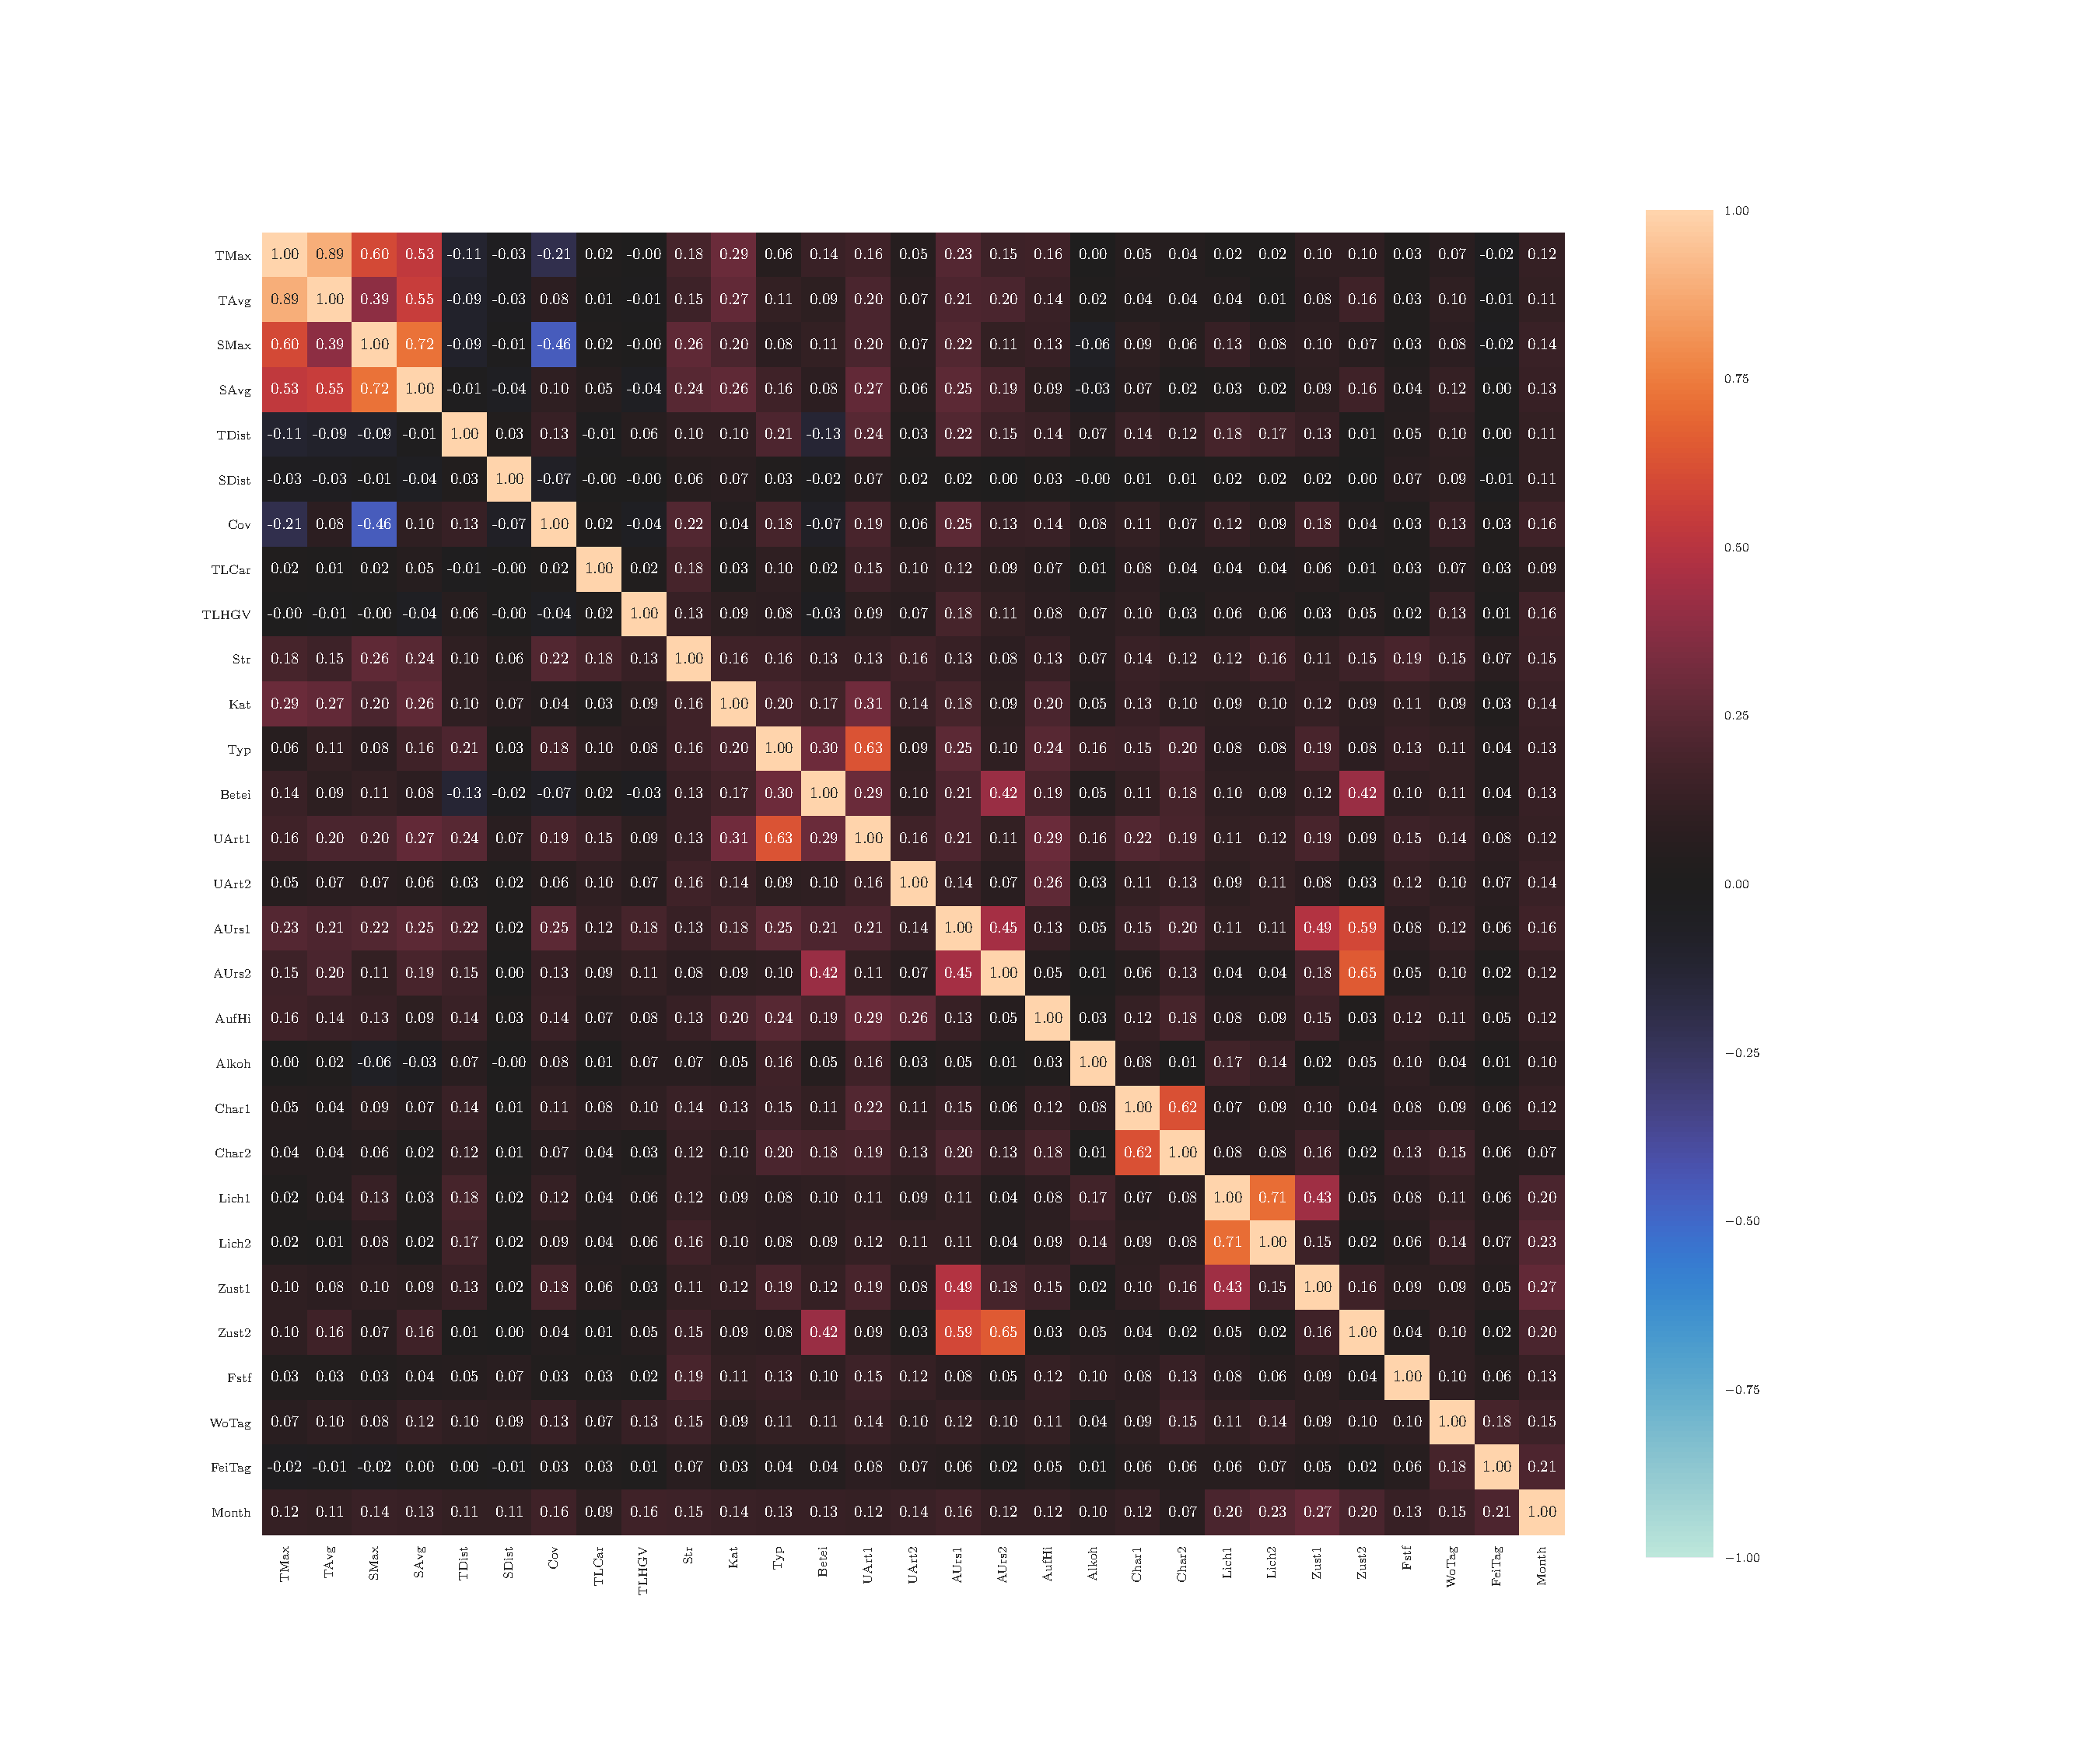
\includegraphics[width=1.4\textwidth, trim=0cm 2.5cm 6cm 3cm]{CorrAnalysis/data/BAYSIS/03_selected_01_startJam/plots/baysis_selected_corr_cramers}%
	}
	\caption{Correlation matrix for congestion-accident matched data classified as \textit{Jam Initiator} and calculated with $V$, $\eta$, $\tau$, $r_{pq}$, $r$}
	\label{img:correlation_matrix_selected_initiator_cramers}
\end{figure}

% --------------------------
% -------- Strasse ---------
% --------------------------
\centerheading{Strasse}
All of the Kruskal-Wallis rank sum test for \textit{Strasse} - \textit{TMax}, \textit{Strasse} - \textit{TAvg}, \textit{Strasse} - \textit{SMax}, \textit{Strasse} - \textit{SAvg}, \textit{Strasse} - \textit{Cov} and \textit{Strasse}-\textit{TLCar} produce a $p$-value above the defined $\alpha$-level of .05. This means that the correlation of the variable \textit{Strasse} can be neglected.

% ----------------------
% -------- Kat ---------
% ----------------------
\centerheading{Kat}
This section analyzes the correlated relations of the variable \textbf{Kat}. The encoding and description of the variable \textbf{Typ} is shown in \cref{tbl:baysis_dataset_Typ}.
% \begin{table}[!ht]
% 	\centering
% 	\tiny
% 	\begin{tabular}{c|l} 
% 		\toprule
% 		Code & Description \\ 
% 		\midrule
%  		0 	& Minor Accident  \\
%  		1 	& Accident with deaths  \\ 
%  		2 	& Accident with heavily injured  \\
%  		3 	& Accident with lightly injured  \\
% 		7 	& Accident with property damage  \\
% 		\bottomrule
% 	\end{tabular}
% 	\caption{Encoding of \textbf{Kat}}
% 	\label{table:analysis_encoding_Kat}
% 	%\vspace{-8mm}
% \end{table}
\paragraph{Maximal spatial Extent}
% chi-squared = 732.27, df = 720
The Kruskal-Wallis rank sum test of \textbf{Kat}-\textbf{SMax} produces a $p$-value of 0.3673, which is above $\alpha=.05$. The null hypothesis can't be rejected and there is no significant difference between the groups of \textbf{Kat}. There are no significant groups to identify.

\paragraph{Average spatial Extent}
% chi-squared = 738.37, df = 727
The Kruskal-Wallis rank sum test of \textbf{Kat}-\textbf{SAvg} produces a $p$-value of 0.3767, which is above $\alpha=.05$. The null hypothesis can't be rejected and there is no significant difference between the groups of \textbf{Kat}. There are no significant groups to identify.

\paragraph{Maximal Temporal Extent}
% chi-squared = 196.02, df = 131
The Kruskal-Wallis rank sum test of \textbf{Kat}-\textbf{TMax} produces a $p$-value of 0.0002, which is below $\alpha=.05$. The null hypothesis can therefore be rejected, which means there is a significant difference between the groups of \textbf{Kat}. To identify the significant groups, a pairwise Wilcoxon $T$-test for \textbf{Kat}-\textbf{TMax} is run, which produces \cref{tbl:wilcoxon_baysis_initiator_Kat_TMax}. 
\begin{table}[ht]
	\centering
	\begin{tabular}{rrrr}
		\toprule  
  		& 1 & 2 & 3 \\ 
  		\midrule    
        2 & 0.00 &  &  \\ 
        3 & 0.00 & 0.00 &  \\ 
        7 & 0.00 & 0.00 & 0.00 \\ 
 		\bottomrule
	\end{tabular}
    \caption{Pairwise Wilcoxon $T$-test for \textit{Kat} and \textit{Maximal Temporal Extent}}
    \label{tbl:wilcoxon_baysis_initiator_Kat_TMax}
\end{table}
The matrix shows that there is a general trend and all groups differ significantly. With the descriptives from \cref{tbl:descriptives_baysis_initiator_Kat_TMax} that the $\bar{x}$ and $\tilde{x}$ increases from group 7 to 1. We can therefore interpret that the maximal duration of jams, created by accidents increases with the gravity of the accident.
\begin{table}[ht]
	\centering
	\begin{tabular}{c|c|c|c|c|c|c|c}
		\toprule  
		Group & $n$ & $\bar{x}$ & $\sigma$ & $\tilde{x}$ & $min$ & $max$ & $\Delta$ \\
        \midrule
        1 & 29  & 290.07 & 190.59 & 255.00 & 27 & 864  & 837 \\ 
        2 & 144 & 156.23 & 119.44 & 120.00 & 9  & 657  & 648 \\ 
        3 & 423 & 121.05 & 105.34 & 99.00  & 9  & 1116 & 1107 \\ 
        7 & 181 & 103.13 & 143.89 & 75.00  & 9  & 1341 & 1332 \\ 
 		\bottomrule
	\end{tabular}
    \caption{Descriptives of the groups of \textit{Kat} and \textit{Maximal Temporal Extent} (Jam Initiator)}
    \label{tbl:descriptives_baysis_initiator_Kat_TMax}
\end{table}

\paragraph{Average temporal Extent}
% chi-squared = 222.52, df = 175
The Kruskal-Wallis rank sum test of \textbf{Kat}-\textbf{TAvg} produces a $p$-value of 0.0087, which is way below $\alpha=.05$. The null hypothesis can therefore be rejected, which means there is a significant difference between the groups of \textbf{Kat}. To identify the significant groups, a pairwise Wilcoxon $T$-test for \textbf{Kat}-\textbf{TAvg} is run, which produces \cref{tbl:wilcoxon_baysis_initiator_Kat_TAvg}. 
\begin{table}[ht]
	\small
	\centering
    \begin{tabular}{rrrr}
        \toprule
        & 1 & 2 & 3 \\ 
        \midrule
        2 & 0.00 &  &  \\ 
        3 & 0.00 & 0.01 &  \\ 
        7 & 0.00 & 0.00 & 0.00 \\ 
        \bottomrule
    \end{tabular}
	\caption{Pairwise Wilcoxon $T$-test for \textit{Kat} and \textit{Average Temporal Extent} (Jam Initiator)}
	\label{tbl:wilcoxon_baysis_initiator_Kat_TAvg}
\end{table}
The $p$-values show that all groups differ significantly from each other. The descriptives in table \cref{tbl:descriptives_baysis_initiator_Kat_TAvg}, show that $\bar{x}$ and $\tilde{x}$ increases with the groups from 7 to 1, like \textbf{TAMx}. The interpretation is therefore similar that the average duration of jams created by accident increases with the gravity of the accident.
\begin{table}[ht]
	\small
	\centering
    \begin{tabular}{c|c|c|c|c|c|c|c}
        \toprule
        Group & $n$ & $\bar{x}$ & $\sigma$ & $\tilde{x}$ & $min$ & $max$ & $\Delta$ \\
        \midrule
        1 & 29  & 148.76 & 90.65 & 144.00 & 20 & 376 & 356 \\ 
        2 & 144 & 80.91  & 67.52 & 61.50  & 7  & 426 & 419 \\ 
        3 & 423 & 63.84  & 51.24 & 53.00  & 5  & 469 & 464 \\ 
        7 & 181 & 53.61  & 80.96 & 39.00  & 4  & 920 & 916 \\ 
        \bottomrule
    \end{tabular}
	\caption{Group descriptives of \textit{Kat} and \textit{Average temporal Extent} (Jam Initiator)}
	\label{tbl:descriptives_baysis_initiator_Kat_TAvg}
	%\vspace{-8mm}
\end{table}

% ----------------------
% -------- Typ ---------
% ----------------------
\Large
\centerline{\textbf{Typ}}
\normalsize
This section analyzes the correlated relations of the accident variable \textbf{Typ} and introduces a initial interpretation of each significant correlation. Groups with an insufficient sample size (see \cref{correlation_uncertainty} are neglected and not considered. The encoding and description of the variable \textbf{Typ} is shown in \cref{tbl:baysis_dataset_Typ}. The relations of \textbf{Kat}-\textbf{SAvg} and 
\textbf{Kat}-\textbf{Cov} produce a $p$-value above the $\alpha$-level in the Kruskal-Wallis rank sum test. The null hypothesis can't therefore be rejected and there is no significant difference between the groups of \textbf{Typ} for these relations. The are also no significant groups to be identified for these relations.

The Kruskal-Wallis rank sum test of \textbf{Kat}-\textbf{TDist} produces a $p$-value of 0.0261, which is way below $\alpha=.05$. The null hypothesis can therefore be rejected, which means there is a significant difference between the groups of \textbf{Kat}. To identify the significant groups, a pairwise Wilcoxon $T$-test for \textbf{Kat}-\textbf{TDist} is run, which produces \cref{tbl:wilcoxon_baysis_initiator_Typ_TDist}. 
\begin{table}[ht]
	\tiny
	\centering
    \begin{tabular}{rrrrrr}
        \toprule
        & 1 & 3 & 4 & 5 & 6 \\ 
        \midrule
        3 & 0.05 &  &  &  &  \\ 
        4 & 1.00 & 0.38 &  &  &  \\ 
        5 & 0.96 & 1.00 & 0.96 &  &  \\ 
        6 & 0.00 & 0.96 & 0.51 & 1.00 &  \\ 
        7 & 1.00 & 0.04 & 1.00 & 0.96 & 0.01 \\ 
        \bottomrule
    \end{tabular}
    \caption{Pairwise Wilcoxon $T$-test for \textit{Typ} and \textit{Temporal Distance} (Jam Initiator)}
    \label{tbl:wilcoxon_baysis_initiator_Typ_TDist}
\end{table}
The significance matrix \cref{tbl:wilcoxon_baysis_initiator_Typ_TDist} shows that group 6 differs from group 1 and group 7 differs from 6. 
\begin{table}[ht]
	\tiny
	\centering
    \begin{tabular}{c|c|c|c|c|c|c|c}
        \toprule
        Group & $n$ & $\bar{x}$ & $\sigma$ & $\tilde{x}$ & $min$ & $max$ & $\Delta$ \\
        \midrule
        1 & 181 & 11.40 & 6.38 & 10.00 & 1  & 24 & 23 \\ 
        3 & 24  & 7.67  & 6.06 & 7.00  & 1  & 22 & 21 \\ 
        %4 & 4   & 14.00 & 3.92 & 13.50 & 10 & 19 & 9 \\ 
        %5 & 2   & 4.50  & 3.54 & 4.50  & 2  & 7  & 5 \\ 
        6 & 496 & 9.20  & 5.88 & 8.00  & 0  & 24 & 24 \\ 
        7 & 70  & 12.27 & 7.09 & 11.00 & 0  & 24 & 24 \\ 
        \bottomrule
    \end{tabular}
    \caption{Group descriptives of \textit{Typ} and \textit{Temporal Distance} (Jam Initiator)}
    \label{tbl:descriptives_baysis_initiator_Typ_TDist}
	%\vspace{-8mm}
\end{table}
The descriptives from \cref{tbl:descriptives_baysis_initiator_Typ_TDist} also shows that the temporal distance in group 1 and 7 is 25\,\% higher than in group 6. Group 3 also shows a substantial gap in $\bar{x}$ but only is barely significance with $p=.05$. Because the groups of $driving$ and $straight traffic$ accidents are very similar, there is no clear interpretation to be drawn.

% ------------------------
% -------- UArt1 ---------
% ------------------------
\centerheading{UArt}
This section analyzes the correlated relations of the accident variable \textbf{UArt} and introduces a initial interpretation of each significant correlation. Groups with an insufficient sample size (see \cref{correlation_uncertainty} are neglected and not considered. The encoding and description of the variable \textbf{UArt} is shown in \cref{tbl:baysis_dataset_UArt}. The Kruskal-Wallis rank sum test of \textbf{UArt1}-\textbf{TAvg}, \textbf{UArt1}-\textbf{SMax}, \textbf{UArt1}-\textbf{SAvg} and \textbf{UArt1}-\textbf{TLCar} produce $p$-values above the $\alpha$-level. This means that the null hypothesis can't be rejected and there is no significant difference between the groups of \textbf{UArt1} in these relations. 

The Kruskal-Wallis rank sum test of \textbf{UArt1}-\textbf{TMax} produces a $p$-value of 0.0015, which is below $\alpha=.05$. The null hypothesis can therefore be rejected, which means there is a significant difference between the groups of \textbf{UArt1}. To identify the significant groups, a pairwise Wilcoxon $T$-test for \textbf{UArt1}-\textbf{TMax} is run, which produces \cref{tbl:wilcoxon_baysis_initiator_UArt_TMax}. 
\begin{table}[ht]
	\tiny
	\centering
    \begin{tabular}{rrrrrrrrrr}
        \toprule
        & 0 & 1 & 2 & 3 & 4 & 5 & 6 & 7 & 8 \\ 
        \midrule
        1 & 1.00 &  &  &  &  &  &  &  &  \\ 
        2 & 1.00 & 1.00 &  &  &  &  &  &  &  \\ 
        3 & 1.00 & 0.04 & 0.00 &  &  &  &  &  &  \\ 
        4 & 1.00 & 1.00 & 1.00 & 1.00 &  &  &  &  &  \\ 
        5 & 1.00 & 1.00 & 1.00 & 1.00 & 1.00 &  &  &  &  \\ 
        6 & 1.00 & 1.00 & 1.00 & 1.00 & 1.00 & 1.00 &  &  &  \\ 
        7 & 0.75 & 0.05 & 0.12 & 1.00 & 1.00 & 1.00 & 1.00 &  &  \\ 
        8 & 1.00 & 0.21 & 0.43 & 1.00 & 1.00 & 1.00 & 1.00 & 1.00 &  \\ 
        9 & 1.00 & 0.43 & 1.00 & 1.00 & 1.00 & 1.00 & 1.00 & 1.00 & 1.00 \\ 
        \bottomrule
      \end{tabular}
    \caption{Pairwise Wilcoxon $T$-test for \textit{UArt1} and \textit{Maximal Temporal Extent} (Jam Initiator)}
    \label{tbl:wilcoxon_baysis_initiator_UArt_TMax}
\end{table}
It shows that only groups 4 and 7 differ significantly from group 1. 
\begin{table}[ht]
	\tiny
	\centering
    \begin{tabular}{c|c|c|c|c|c|c|c}
        \toprule
        Group & $n$ & $\bar{x}$ & $\sigma$ & $\tilde{x}$ & $min$ & $max$ & $\Delta$ \\
        \midrule
        % total: 777
        0 & 24  & 140.75 & 100.75 & 114.00 & 30 & 375  & 345 \\ 
        1 & 31  & 198.58 & 166.25 & 126.00 & 39 & 612  & 573 \\ 
        2 & 345 & 134.87 & 108.69 & 105.00 & 9  & 864  & 855  \\ 
        3 & 144 & 111.79 & 123.13 & 81.00  & 9  & 1116 & 1107 \\ 
        %4 & 4   & 186.00 & 145.68 & 175.50 & 39 & 354  & 315 \\ 
        5 & 15  & 179.60 & 324.31 & 99.00  & 15 & 1341 & 1326 \\ 
        %6 & 4   & 171.00 & 98.62  & 178.50 & 66 & 261  & 195 \\ 
        7 & 23  & 87.91  & 93.15  & 48.00  & 12 & 384  & 372 \\ 
        8 & 107 & 118.46 & 117.62 & 87.00  & 18 & 813  & 795 \\ 
        9 & 80  & 122.47 & 143.91 & 91.50  & 12 & 1152 & 1140 \\ 
        \bottomrule
      \end{tabular}
    \caption{Group descriptives of \textit{UArt1} and \textit{Maximal Temporal Extent} (Jam Initiator)}
    \label{tbl:descriptives_baysis_initiator_UArt_TMax}
	%\vspace{-8mm}
\end{table}
Because group 4 only contains 4 samples (see \cref{tbl:descriptives_baysis_initiator_UArt_TMax}) it is considered uncertain (see \cref{correlation_uncertainty}).

The Kruskal-Wallis rank sum test of \textbf{UArt1}-\textbf{TDist} produces a $p$-value of 0.0084, which is below $\alpha=.05$. The null hypothesis can therefore be rejected, which means there is a significant difference between the groups of \textbf{UArt1}. To identify the significant groups, a pairwise Wilcoxon $T$-test for \textbf{UArt1}-\textbf{TDist} is run, which produces \cref{tbl:wilcoxon_baysis_initiator_UArt_TDist}. 
\begin{table}[ht]
	\tiny
	\centering
    \begin{tabular}{rrrrrrrrrr}
        \toprule
        & 0 & 1 & 2 & 3 & 4 & 5 & 6 & 7 & 8 \\ 
        \midrule
        1 & 1.00 &  &  &  &  &  &  &  &  \\ 
        2 & 1.00 & 1.00 &  &  &  &  &  &  &  \\ 
        3 & 1.00 & 1.00 & 1.00 &  &  &  &  &  &  \\ 
        4 & 1.00 & 1.00 & 1.00 & 1.00 &  &  &  &  &  \\ 
        5 & 1.00 & 1.00 & 1.00 & 1.00 & 1.00 &  &  &  &  \\ 
        6 & 1.00 & 1.00 & 1.00 & 1.00 & 1.00 & 1.00 &  &  &  \\ 
        7 & 1.00 & 0.06 & 0.00 & 0.00 & 1.00 & 0.10 & 1.00 &  &  \\ 
        8 & 1.00 & 1.00 & 0.01 & 0.01 & 1.00 & 1.00 & 1.00 & 1.00 &  \\ 
        9 & 1.00 & 1.00 & 0.05 & 0.01 & 1.00 & 0.78 & 1.00 & 0.87 & 1.00 \\ 
        \bottomrule
      \end{tabular}
    \caption{Pairwise Wilcoxon $T$-test for \textit{UArt1} and \textit{Temporal Distance} (Jam Initiator)}
    \label{tbl:wilcoxon_baysis_initiator_UArt_TDist}
\end{table}
The table shows, that groups 7, 8 and 9 differ from group 2 and 3.
\begin{table}[ht]
	\tiny
	\centering
    \begin{tabular}{c|c|c|c|c|c|c|c}
        \toprule
        Group & $n$ & $\bar{x}$ & $\sigma$ & $\tilde{x}$ & $min$ & $max$ & $\Delta$ \\
        \midrule
        0 & 24  & 11.04 & 6.22 & 10.00 & 2  & 22 & 20 \\ 
        1 & 31  & 8.94  & 6.03 & 7.00  & 0  & 24 & 24 \\ 
        2 & 345 & 9.21  & 5.90 & 8.00  & 1  & 24 & 23 \\ 
        3 & 144 & 8.80  & 6.03 & 7.00  & 1  & 24 & 23 \\ 
        %4 & 4   & 12.00 & 4.08 & 10.50 & 9  & 18 & 9  \\ 
        5 & 15  & 8.13  & 7.06 & 7.00  & 0  & 22 & 22 \\ 
        %6 & 4   & 14.00 & 3.92 & 13.50 & 10 & 19 & 9  \\ 
        7 & 23  & 15.26 & 7.04 & 14.00 & 4  & 24 & 20 \\ 
        8 & 107 & 11.81 & 6.57 & 11.00 & 1  & 24 & 23 \\ 
        9 & 80  & 11.38 & 5.87 & 10.00 & 2  & 24 & 22 \\ 
        \bottomrule
      \end{tabular}
    \caption{Group descriptives of \textit{UArt1} and \textit{Temporal Distance}}
    \label{tbl:descriptives_baysis_initiator_UArt_TDist}
	%\vspace{-8mm}
\end{table}
In consideration of the descriptives in \cref{tbl:descriptives_baysis_initiator_UArt_TDist} it can be interpreted that accidents with \textit{obstacles collision}, \textit{deviations to the right} and \textit{deviations to the left} have a longer (temporal) reaction (see distribution of $\bar{x}$) to create a jam than accident with ahead vehicles.

The Kruskal-Wallis rank sum test of \textbf{UArt1}-\textbf{Cov} produces a $p$-value of 0.0337, which is below $\alpha$-level. The null hypothesis can therefore be rejected, which means there are significant differences in \textbf{UArt}. To identify the significant groups the a pairwise Wilcoxon $T$-test for \textbf{UArt1}-\textbf{Cov}, produces \cref*{tbl:wilcoxon_baysis_initiator_UArt_Cov}. It shows that the significant differences are not related to any specific group of \textbf{UArt1} and the correlation can be neglected.
\begin{table}[ht]
	\tiny
	\centering
    \begin{tabular}{rrrrrrrrrr}
        \toprule
        & 0 & 1 & 2 & 3 & 4 & 5 & 6 & 7 & 8 \\ 
        \midrule
        1 & 1.00 &  &  &  &  &  &  &  &  \\ 
        2 & 1.00 & 1.00 &  &  &  &  &  &  &  \\ 
        3 & 1.00 & 1.00 & 1.00 &  &  &  &  &  &  \\ 
        4 & 1.00 & 1.00 & 1.00 & 1.00 &  &  &  &  &  \\ 
        5 & 1.00 & 1.00 & 1.00 & 1.00 & 1.00 &  &  &  &  \\ 
        6 & 1.00 & 1.00 & 1.00 & 1.00 & 1.00 & 1.00 &  &  &  \\ 
        7 & 1.00 & 1.00 & 1.00 & 1.00 & 1.00 & 1.00 & 1.00 &  &  \\ 
        8 & 1.00 & 1.00 & 0.12 & 0.09 & 1.00 & 0.72 & 1.00 & 1.00 &  \\ 
        9 & 1.00 & 1.00 & 1.00 & 1.00 & 1.00 & 1.00 & 1.00 & 1.00 & 1.00 \\ 
        \bottomrule
      \end{tabular}
    \caption{Pairwise Wilcoxon $T$-test for \textit{UArt1} and \textit{Coverage} (Jam Initiator)}
    \label{tbl:wilcoxon_baysis_initiator_UArt_Cov}
\end{table}

% ------------------------
% -------- AUrs1 ---------
% ------------------------
\centerheading{AUrs}
This section analyzes the correlated relations of the accident variable \textbf{AUrs1} and \textbf{AUrs2}, also introducing a initial interpretation of each significant correlation. Groups with an insufficient sample size (see \cref{correlation_uncertainty} are neglected and not considered. The encoding and description of the variable \textbf{AUrs} is shown in \cref{tbl:baysis_dataset_AUrs}. The Kruskal-Wallis rank sum test of \textbf{AUrs1}-\textbf{TMax}, \textbf{AUrs1}-\textbf{TAvg}, \textbf{AUrs1}-\textbf{SMax}, \textbf{AUrs1}-\textbf{SAvg}, \textbf{AUrs1}-\textbf{TDist} and \textbf{AUrs1}-\textbf{TLCar} produce $p$-values above the $\alpha$-level. This means that the null hypothesis can't be rejected and there is no significant difference between the groups of \textbf{UArt1} in these relations. 

The Kruskal-Wallis rank sum test of \textbf{AUrs1}-\textbf{Cov} produces a $p$-value of 0.0176, which is below $\alpha=.05$. The null hypothesis can therefore be rejected, pointing to a significant difference between the groups of \textbf{AUrs1}. The pairwise Wilcoxon $T$-test of \textbf{AUrs1}-\textbf{Cov} for identification of the relevant groups (see \cref{tbl:wilcoxon_baysis_initiator_AUrs1_Cov}) shows that the significance differences is not group specific. The correlation can therefore be neglected.
\begin{table}[ht]
	\small
	\centering
    \begin{tabular}{rrrrrrrrrrrrr}
        \toprule
           & 72 & 73 & 75 & 77 & 81 & 82 & 83 & 84 & 86 & 87 & 88 \\ 
        \midrule
        72 &  &  &  &  &  &  &  &  &  &  &  \\ 
        73 & 0.63 &  &  &  &  &  &  &  &  &  &  \\ 
        75 & 1.00 & 1.00 &  &  &  &  &  &  &  &  &  \\ 
        77 & 1.00 & 1.00 & 1.00 &  &  &  &  &  &  &  &  \\ 
        81 & 1.00 & 1.00 & 1.00 & 1.00 &  &  &  &  &  &  &  \\ 
        82 & 1.00 & 1.00 & 1.00 & 1.00 & 1.00 &  &  &  &  &  &  \\ 
        83 & 1.00 & 1.00 & 1.00 & 1.00 & 1.00 & 1.00 &  &  &  &  &  \\ 
        84 & 1.00 & 1.00 & 1.00 & 1.00 & 1.00 & 1.00 & 1.00 &  &  &  &  \\ 
        86 & 1.00 & 1.00 & 1.00 & 1.00 & 1.00 & 1.00 & 1.00 & 1.00 &  &  &  \\ 
        87 & 1.00 & 1.00 & 1.00 & 1.00 & 1.00 & 1.00 & 1.00 & 1.00 & 1.00 &  &  \\ 
        88 & 1.00 & 1.00 & 1.00 & 1.00 & 1.00 & 1.00 & 1.00 & 1.00 & 1.00 & 1.00 &  \\ 
        89 & 0.33 & 0.96 & 1.00 & 1.00 & 1.00 & 1.00 & 1.00 & 1.00 & 0.91 & 1.00 & 1.00 \\ 
        \bottomrule
    \end{tabular}
    \caption{Pairwise Wilcoxon $T$-test for \textit{AUrs1} and \textit{Coverage} (Jam Initiator)}
    \label{tbl:wilcoxon_baysis_initiator_AUrs1_Cov}
\end{table}

% ------------------------
% -------- AUrs2 ---------
% ------------------------
\medskip
All relations of the second \textbf{AUrs} variable \textbf{AUrs2} (\textbf{AUrs2}-\textbf{TMax}, \textbf{AUrs2}-\textbf{TAvg}, \textbf{AUrs2}-\textbf{SAvg} and \textbf{AUrs2}-\textbf{TDist}) produce $p$-values above $\alpha$-level. The null hypothesizes can't be rejected and there is no significant differences between the groups of \textbf{AUrs2}. There are therefore no significant groups to identify.

% ------------------------
% -------- AufHi ---------
% ------------------------
\centerheading{AufHi}
This section analyzes the correlated relations of the accident variable \textit{AufHi}. The relations of \textit{AufHi}-\textit{TAvg} and \textit{AufHi}-\textit{Cov} produce a $p$-value above the $\alpha$-level. The null hypothesizes can't be rejected and there are no significant differences between the groups of \textit{AufHi} for these relations.

The Kruskal-Wallis rank sum tests of \textit{AufHi} - \textit{TMax} produces a $p$-value of 0.0411, which is below $\alpha=.05$. The null hypothesis can therefore be rejected, which means there is a significant difference between the groups of \textit{AufHi}. The pairwise Wilcoxon $T$-test for \textit{AufHi} - \textit{TMax} shows no significant differences between the groups, which mean that the correlation can be neglected.

The Kruskal-Wallis rank sum test of \textit{AufHi} - \textit{TDist} produces a $p$-value of 0.0007, which is below $\alpha=.05$. The null hypothesis can therefore be rejected, which means there is a significant difference between the groups of \textit{AufHi}. The pairwise Wilcoxon $T$-test for \textit{AufHi} - \textit{TDist} shows no significant differences between the groups.

% ------------------------
% -------- Char1 ---------
% ------------------------
\centerheading{Char}
This section analyzes the correlated relations of the accident variable \textit{Char}. The relations of \textit{Char1}-\textit{TDist} produces a $p$-value above the $\alpha$-level. The null hypothesis can't be rejected and there is no significant difference between the groups of \textit{Char1}. There are therefore also no significant groups to identify.

% --------------------------------
% -------- Lich1 & Lich2 ---------
% --------------------------------
\centerheading{Lich}
This section analyzes the correlated relations of the accident variable \textit{Lich1} as well as \textit{Lich2}. The relations of \textit{Lich1}-\textit{TDist} and \textit{Lich2}-\textit{TDist} produce a $p$-value above the $\alpha$-level. The null hypothesizes can't be rejected and there are no significant differences between the groups of \textit{Lich1} and \textit{Lich2}.

% ------------------------
% -------- Zust1 ---------
% ------------------------
\centerheading{Zust}
This section analyzes the correlated relations of the accident variable \textit{Zust1}/\textit{Zust2} and introduces a initial interpretation of each significant correlation. The encoding and description of the variable \textit{Zust} is shown in \cref{tbl:baysis_dataset_Zust}. The relations of \textit{Zust2} - \textit{SAvg} produce a $p$-value above $\alpha=.05$. The null hypothesizes can't be rejected and there are no significant differences between the groups of \textit{Zust2}. The Kruskal-Wallis rank sum test of \textit{Zust2} - \textit{TAvg} produces a $p$-value of < 0.0001, which is significant. But because the distribution only contains a single values, there are no interpretations to be draw and the correlation can be neglected.

The Kruskal-Wallis rank sum test of \textit{Zust1} - \textit{Cov} produces a $p$-value of 0.0046, which is way below $\alpha=.05$. The null hypothesis can therefore be rejected, which means there is a significant difference between the groups of \textit{Zust1}. To identify the significant groups, a pairwise Wilcoxon $T$-test for \textit{Zust1} - \textit{Cov} is run, which produces \cref{tbl:wilcoxon_baysis_initiator_Zust1_Cov}. 
\begin{table}[ht!]
	\tiny
	\centering
    \begin{tabular}{rrrr}
        \toprule
          & 0 & 1 \\ 
        \midrule
        0 &      & \\ 
        1 & 0.04 & \\ 
        2 & 0.00 & 0.01 \\ 
        \bottomrule
      \end{tabular}
    \caption{Pairwise Wilcoxon $T$-test for \textit{Zust1} and \textit{Coverage}}
    \label{tbl:wilcoxon_baysis_initiator_Zust1_Cov}
\end{table}
The table shows that all groups differ significantly, which means that there is a general trend.
\begin{table}[ht!]
	\tiny
	\centering
    \begin{tabular}{c|c|c|c|c|c|c|c}
        \toprule
        Group & $n$ & $\bar{x}$ & $\sigma$ & $\tilde{x}$ & $min$ & $max$ & $\Delta$ \\
        \midrule
        0 & 548 & 50.80 & 20.28 & 49.50 & 6  & 100 & 94 \\ 
        1 & 208 & 55.35 & 21.35 & 55.00 & 5  & 100 & 95 \\ 
        2 & 18  & 74.06 & 26.80 & 87.50 & 18 & 100 & 82 \\ 
        \bottomrule
      \end{tabular}
    \caption{Group descriptives of \textit{Zust1} and \textit{Coverage}}
    \label{tbl:descriptives_baysis_initiator_Zust1_Cov}
	%\vspace{-8mm}
\end{table}
With the descriptives in \cref*{tbl:descriptives_baysis_initiator_Zust1_Cov} it can be interpreted that the coverage of the jam increases from \textit{dry} over \textit{wet} to \textit{ice} by nearly 50\,\%.

% ------------------------
% -------- Month ---------
% ------------------------
\centerheading{Month}
This section analyzes the correlated relations of the accident variable \textit{Month}. The relations of \textit{Month} - \textit{TMax}, \textit{Month} - \textit{Cov} and \textit{Month} - \textit{TLHGV} produce a $p$-value above the $\alpha$-level. The null hypothesizes can't be rejected and there are \textit{no} significant differences between the groups of \textit{Month} for the mentioned relations. There are no significant groups to identify.
\clearpage
% Effector
% ----------------------------------------------------
% -------- BAYSIS - Selected as Jam Effector ---------
% ----------------------------------------------------
\subsection{Congestion - Accidents categorizes as Jam Effector}
\label{analysis_processing_correlation_baysis_effector}
The correlation matrix table for the congestion - accident dataset, which are classified as \textit{Jam Effector} (see \cref{table:appendix_correlation_matrix_matched_cramers}) is visual presented in \cref{img:correlation_matrix_selected_effector_cramers} showing the the correlation of each variable combination. When visual analyzing \cref{img:correlation_matrix_matched_cramers} and checking the guidelines for a strong correlation in reference to the applied coefficient (identifiable with \cref{table:appendix_coefficient_matrix_matched}) we get a list of strongly correlated variable combinations (see \cref{tbl:correlation_list_baysis_effector}). Since the focus of the thesis are the correlations between accidents and jams, these are only collected from the bottom-left rectangle of the matrix, where the congestion and accidents variables intersect. Correlations of the kind congestion - congestion or accident - accident are not considered.
\begin{table}[h!]
	\centering
	\begin{tabular}{c|l}  
		Category & Strong \\
		\\[-1em]
		\hline
		\\[-1em]
		Strasse & TMax, TAvg, SMax, SAvg, Cov, TLHGV \\ 
 		Kat & TMax, TAvg, SAvg \\ % + SMax % -> Strasse
 		%Typ & \\ % -> Strasse
 		%Betei & \\
 		UArt1 & SAvg \\ % -> Strasse
 		%UArt2 & \\ % -> Strasse
 		%AUrs1 & \\ % -> Strasse
 		%AUrs2 & \\
 		AufHi & TMax, TAvg \\
 		%Alkoh & \\
 		%Char1 & \\ % -> Strasse
 		%Char2 & \\ % -> Strasse
 		%Lich1 & \\ % -> Strasse
 		%Lich2 & \\ % -> Strasse
 		%Zust1 & \\ % -> Strasse
 		%Zust2 & \\ % -> Strasse
 		%Fstf & \\ % -> Strasse
 		WoTag & TAvg, SMax, Cov, TLHGV \\ % -> Strasse
 		%FeiTag & \\
 		Month & TMax, TAvg, SMax, SAvg, Cov, TLHGV \\ % -> Strasse
	\end{tabular}
    \caption{List of incident variables and their strong correlated congestion variable from the congestion-accident matched data which are classified as \textit{Jam Effector}}
	\label{tbl:correlation_list_baysis_effector}
\end{table}
Next we need to verify that the correlation is significant and what the correlation predicates. Therefore each correlation will be evaluated with the Post Hoc test, defined in \cref{correlation_posthoc}. \secintroend{baysis}{effector}
\begin{figure}[!ht]
	\centering
	\makebox[\textwidth][c]{%
		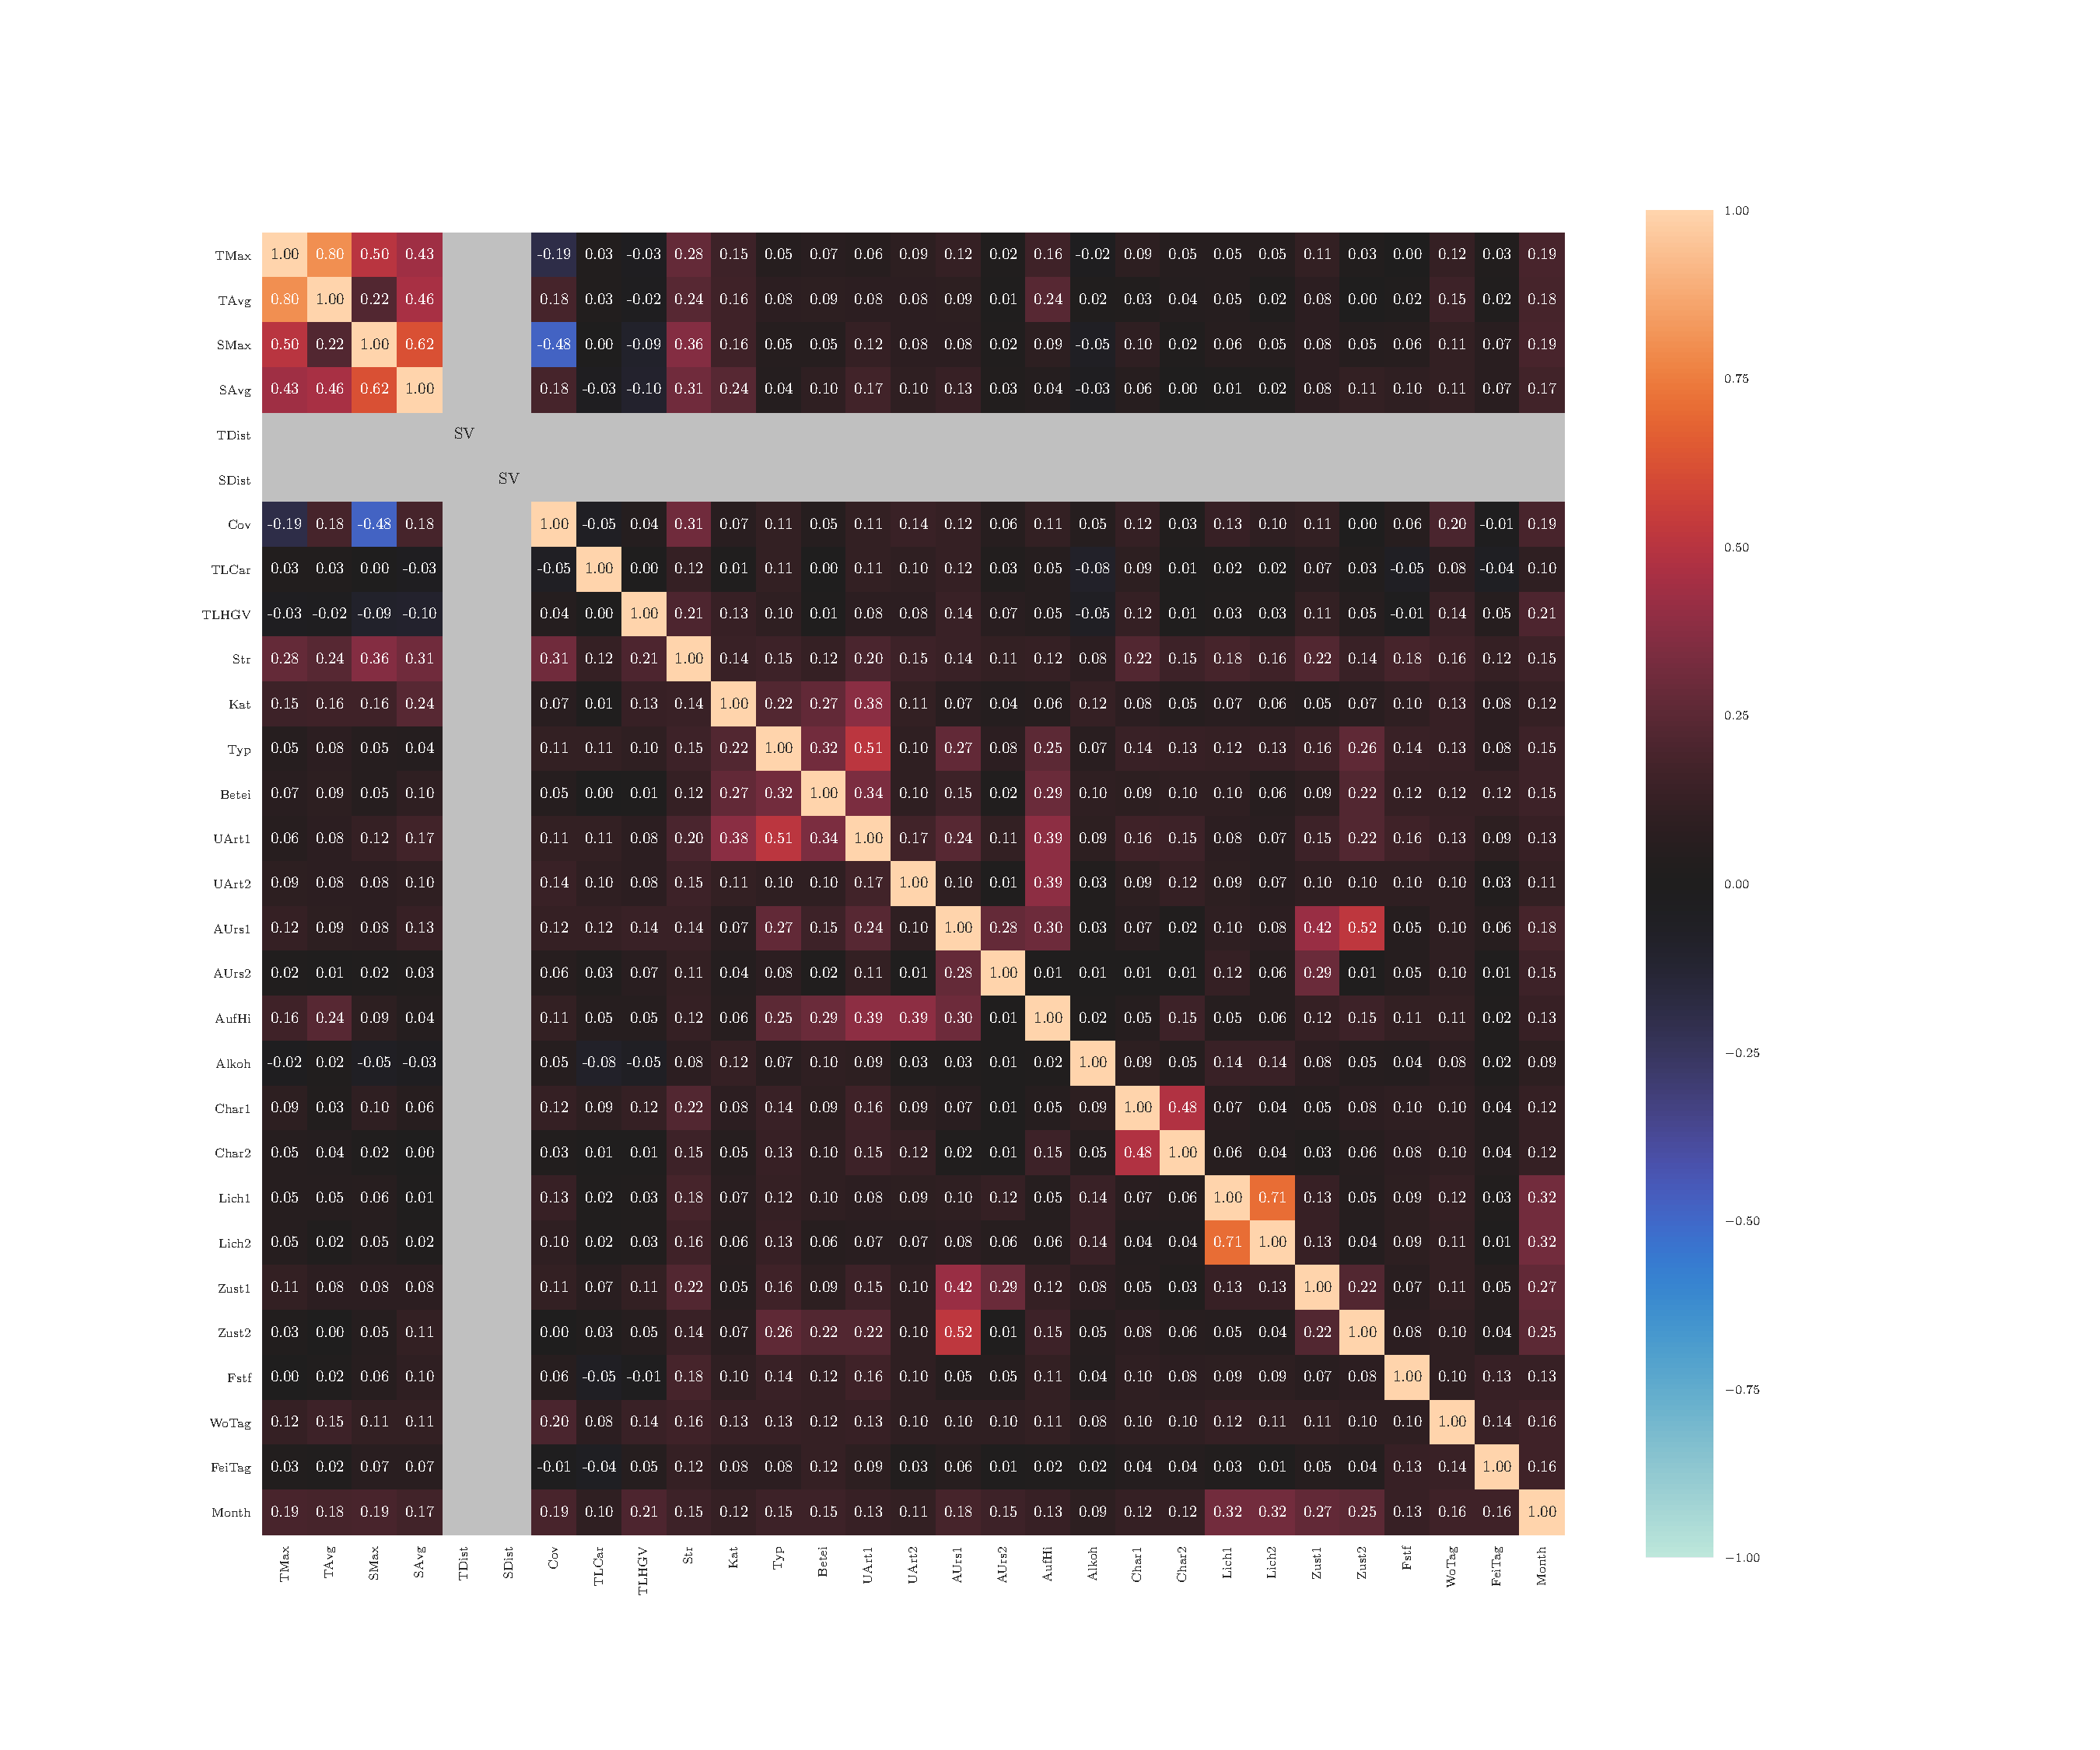
\includegraphics[width=1.4\textwidth, trim=0cm 2.5cm 6cm 3cm]{CorrAnalysis/data/BAYSIS/03_selected_02_duringJam/plots/baysis_selected_corr_cramers}%
	}
	\caption{Correlation matrix for congestion-accident matched data classified as \textit{Jam Effector} and calculated with $V$, $\eta$, $\tau$, $r_{pq}$, $r$}
	\label{img:correlation_matrix_selected_effector_cramers}
\end{figure}

% --------------------------
% -------- Street ---------
% --------------------------
\centerheading{Street}
\label{ana:baysis_effector_Str}
\varintrosimplewithsam{Str}
\varintronosigmul{Str}{\textit{Strasse} - \textit{SAvg} and \textit{Strasse} - \textit{TLHGV}}

% #################################################
\groupintrosig{Street}{TMax}{0.0104}{baysis}{effector}
\begin{table}[ht!]
	\tiny
	\centering
	\begin{tabular}{rrrrrrrrrrrrrr}
		\toprule
		     & A3 & A6 & A9 & A70 & A99 & A93 & A94 & A7 & A73 & A96 & A995 & A92 & A95 \\ 
		\midrule
		% A6   & 1.00 &  &  &  &  &  &  &  &  &  &  &  &  \\ 
		% A9   & 1.00 & 1.00 &  &  &  &  &  &  &  &  &  &  &  \\ 
		% A70  & 1.00 & 1.00 & 1.00 &  &  &  &  &  &  &  &  &  &  \\ 
		% A99  & 0.85 & 1.00 & 1.00 & 1.00 &  &  &  &  &  &  &  &  &  \\ 
		% A93  & 1.00 & 1.00 & 1.00 & 1.00 & 1.00 &  &  &  &  &  &  &  &  \\ 
		A94  & \red{0.01} & 1.00 & 0.06 & 1.00 & 0.28 & 1.00 &  &  &  &  &  &  &  \\ 
		% A7   & .00 & 1.00 & 1.00 & 1.00 & 1.00 & 1.00 & 1.00 &  &  &  &  &  &  \\ 
		A73  & \red{0.00} & 1.00 & \red{0.00} & 1.00 & 0.23 & 1.00 & 1.00 & 1.00 &  &  &  &  &  \\ 
		A96  & \red{0.00} & 1.00 & 0.35 & 1.00 & 1.00 & 1.00 & 1.00 & 1.00 & 1.00 &  &  &  &  \\ 
		% A995 & 1.00 & 1.00 & 1.00 & 1.00 & 1.00 & 1.00 & 1.00 & 1.00 & 1.00 & 1.00 &  &  &  \\ 
		A92  & \red{0.01} & 1.00 & 0.24 & 1.00 & 1.00 & 1.00 & 1.00 & 1.00 & 1.00 & 1.00 & 1.00 &  &  \\ 
		% A95  & 1.00 & 1.00 & 1.00 & 1.00 & 1.00 & 1.00 & 1.00 & 1.00 & 1.00 & 1.00 & 1.00 & 1.00 &  \\ 
		% A980 & 1.00 & 1.00 & 1.00 & 1.00 & 1.00 & 1.00 & 1.00 & 1.00 & 1.00 & 1.00 & 1.00 & 1.00 &  \\ 
		\bottomrule
	  \end{tabular}
    \caption{Pairwise Wilcoxon $T$-test for \textit{Street} and \textit{Maximal Temporal Extent} (Jam Effector)}
    \label{tbl:wilcoxon_baysis_effector_Street_TMax}
\end{table}
The table shows that the roads A73, A94, A95 and A96 differ from the A3. The A73 also differs from the A9, but there is no distinctive general trend.
% #### START: Table and Plot
\begin{figure}[ht!]
	\centering
	\begin{minipage}{0.5\textwidth}
		\tiny
		\setlength{\tabcolsep}{4pt}
		\centering
		\begin{tabular}{c|c|c|c|c|c|c|c}
			\toprule
			Group & $n$ & $\bar{x}$ & $\sigma$ & $\tilde{x}$ & $min$ & $max$ & $\Delta$ \\
			\midrule
			A3   & 265 & 297.62 & 219.09 & 243.0 & 18 & 1257 & 1239 \\ 
			A6   & 37  & 236.59 & 183.03 & 207.0 & 18 & 705  & 687  \\ 
			A9   & 192 & 243.45 & 178.97 & 201.0 & 15 & 1194 & 1179 \\ 
			A99  & 63  & 212.57 & 140.78 & 195.0 & 21 & 681  & 660  \\ 
			A93  & 12  & 212.00 & 187.74 & 130.5 & 39 & 588  & 549  \\ 
			A94  & 14  & 109.71 & 56.07  & 97.5  & 42 & 249  & 207  \\ 
			A7   & 35  & 254.66 & 306.21 & 168.0 & 42 & 1341 & 1299 \\ 
			A73  & 52  & 157.21 & 179.42 & 130.5 & 18 & 1323 & 1305 \\ 
			A96  & 41  & 155.85 & 84.33  & 144.0 & 30 & 381  & 351  \\ 
			A92  & 21  & 134.71 & 82.25  & 138.0 & 18 & 354  & 336  \\ 
			\bottomrule
			% \bar{x} - sum = 2014.37, mean = 201,43
			% \sigma - sum = 1617.89, mean = 161.78
			% \tilde{x}
		\end{tabular}
		\subcaption[second caption.]{Table of all descriptives}\label{tbl:descriptives_baysis_effector_Street_TMax}
	\end{minipage}%
	\begin{minipage}{0.55\textwidth}
		\pgfplotstableread[col sep=comma]{
			road, count, mean, median, sd, min, max, delta
			A3   , 265 , 297.62 , 219.09 , 243.0 , 18 , 1257 , 1239
			A6   , 37  , 236.59 , 183.03 , 207.0 , 18 , 705  , 687 
			A9   , 192 , 243.45 , 178.97 , 201.0 , 15 , 1194 , 1179
			A99  , 63  , 212.57 , 140.78 , 195.0 , 21 , 681  , 660 
			A93  , 12  , 212.00 , 187.74 , 130.5 , 39 , 588  , 549 
			A94  , 14  , 109.71 , 56.07  , 97.5  , 42 , 249  , 207 
			A7   , 35  , 254.66 , 306.21 , 168.0 , 42 , 1341 , 1299
			A73  , 52  , 157.21 , 179.42 , 130.5 , 18 , 1323 , 1305
			A96  , 41  , 155.85 , 84.33  , 144.0 , 30 , 381  , 351 
			A92  , 21  , 134.71 , 82.25  , 138.0 , 18 , 354  , 336 
		}\data
        \pgfplotstablesort[sort key=mean, sort cmp=float >]{\datasorted}{\data}
        \tiny
        \centering
        \descplotfigwithavg{\datasorted}{201}{161}{9}{4.7}
		\subcaption[second caption.]{Plot of descriptives $\bar{x}$, $\sigma$ and $\tilde{x}$}\label{fig:descriptives_baysis_effector_Street_TMax}
	\end{minipage}%
	\caption{Group descriptives of \textit{Street} and \textit{Maximal Temporal Extent} (Jam Effector)}
	%\vspace{-8mm}
\end{figure}
% #### END: Table and Plot
The significant descriptives from \cref{tbl:descriptives_baysis_effector_Street_TMax,fig:descriptives_baysis_effector_Street_TMax} that the mean of A3 is 140\,min - 188\,min higher than the means of A73, A94, A95 and A96. They also show that the mean of A73 is 86\,min lower than the mean of A9. Therefore it can be interpreted that accidents on the A3 and A9 are associated with significantly longer (temporal) jams than on the A73, A94, A95 and A96. The descriptives also show that the A73, A92, A94 and A96 are have considerable shorter durations, when the A3, A6, A7 and A9 have considerable longer durations compared to the general mean.
\groupintrosig{Street}{TAvg}{0.0003}{baysis}{effector}
\begin{table}[ht!]
	\tiny
	\centering
	\begin{tabular}{rrrrrrrrrrrrrr}
		\toprule
			 & A3 & A6 & A9 & A70 & A99 & A93 & A94 & A7 & A73 & A96 & A995 & A92 & A95 \\ 
		\midrule
		% A6   & 1.00 &  &  &  &  &  &  &  &  &  &  &  &  \\ 
		% A9   & 1.00 & 1.00 &  &  &  &  &  &  &  &  &  &  &  \\ 
		% A70  & 1.00 & 1.00 & 1.00 &  &  &  &  &  &  &  &  &  &  \\ 
		A99  & \red{0.02} & 1.00 & 1.00 & 1.00 &  &  &  &  &  &  &  &  &  \\ 
		% A93  & 1.00 & 1.00 & 1.00 & 1.00 & 1.00 &  &  &  &  &  &  &  &  \\ 
		% A94  & 0.11 & 1.00 & 0.53 & 1.00 & 1.00 & 1.00 &  &  &  &  &  &  &  \\ 
		% A7   & 1.00 & 1.00 & 1.00 & 1.00 & 1.00 & 1.00 & 0.61 &  &  &  &  &  &  \\ 
		A73  & \red{0.00} & 1.00 & 0.00 & 1.00 & 1.00 & 1.00 & 1.00 & \red{0.02} &  &  &  &  &  \\ 
		% A96  & 1.00 & 1.00 & 1.00 & 1.00 & 1.00 & 1.00 & 1.00 & 1.00 & 0.87 &  &  &  &  \\ 
		% A995 & 1.00 & 1.00 & 1.00 & 1.00 & 1.00 & 1.00 & 1.00 & 1.00 & 1.00 & 1.00 &  &  &  \\ 
		% A92  & 1.00 & 1.00 & 1.00 & 1.00 & 1.00 & 1.00 & 1.00 & 1.00 & 1.00 & 1.00 & 1.00 &  &  \\ 
		% A95  & 1.00 & 1.00 & 1.00 & 1.00 & 1.00 & 1.00 & 1.00 & 1.00 & 1.00 & 1.00 & 1.00 & 1.00 &  \\ 
		% A980 & 1.00 & 1.00 & 1.00 & 1.00 & 1.00 & 1.00 & 1.00 & 1.00 & 1.00 & 1.00 & 1.00 & 1.00 & 1.00 \\ 
		\bottomrule
	  \end{tabular}
    \caption{Pairwise Wilcoxon $T$-test for \textit{Strasse} and \textit{Average Temporal Extent} (Jam Effector)}
    \label{tbl:wilcoxon_baysis_effector_Street_TAvg}
\end{table}
The table shows that the roads A99 and A73 differ significantly from the A3. The A73 also differs significantly from A7.
% #### START: Table and Plot
\begin{figure}[ht!]
	\centering
	\begin{minipage}{0.5\textwidth}
		\tiny
		\centering
		\begin{tabular}{c|c|c|c|c|c|c|c}
			\toprule
			Group & $n$ & $\bar{x}$ & $\sigma$ & $\tilde{x}$ & $min$ & $max$ & $\Delta$ \\
			\midrule
			A3   & 265 & 104.05 & 87.02  & 84 & 7  & 703  & 696  \\ 
			A6   & 37  & 82.43  & 74.19  & 70 & 3  & 301  & 298  \\ 
			A9   & 192 & 91.31  & 74.64  & 75 & 5  & 575  & 570  \\  
			A99  & 63  & 65.73  & 47.32  & 52 & 4  & 295  & 291  \\ 
			A93  & 12  & 104.83 & 112.03 & 55 & 7  & 343  & 336  \\ 
			A94  & 14  & 45.93  & 25.54  & 43 & 14 & 102  & 88   \\ 
			A7   & 35  & 143.74 & 255.78 & 76 & 15 & 1326 & 1311 \\ 
			A73  & 52  & 47.63  & 29.09  & 44 & 6  & 154  & 148  \\ 
			A96  & 41  & 74.39  & 54.53  & 70 & 6  & 247  & 241  \\ 
			A92  & 21  & 64.52  & 48.86  & 56 & 8  & 235  & 227  \\ 
			\bottomrule
			% \bar{x} - sum = 824.56, mean = 82.45
			% \sigma - sum = 809, mean = 80.9
			% \tilde{x}
		\end{tabular}
		\subcaption[second caption.]{Table of all descriptives}\label{tbl:descriptives_baysis_effector_Street_TAvg}
	\end{minipage}%
	\begin{minipage}{0.55\textwidth}
		\pgfplotstableread[col sep=comma]{
			road, count, mean, median, sd, min, max, delta
			A3   , 265 , 104.05 , 87.02  , 84 , 7  , 703  , 696 
			A6   , 37  , 82.43  , 74.19  , 70 , 3  , 301  , 298 
			A9   , 192 , 91.31  , 74.64  , 75 , 5  , 575  , 570  
			A99  , 63  , 65.73  , 47.32  , 52 , 4  , 295  , 291 
			A93  , 12  , 104.83 , 112.03 , 55 , 7  , 343  , 336 
			A94  , 14  , 45.93  , 25.54  , 43 , 14 , 102  , 88  
			A7   , 35  , 143.74 , 255.78 , 76 , 15 , 1326 , 1311
			A73  , 52  , 47.63  , 29.09  , 44 , 6  , 154  , 148 
			A96  , 41  , 74.39  , 54.53  , 70 , 6  , 247  , 241 
			A92  , 21  , 64.52  , 48.86  , 56 , 8  , 235  , 227 
		}\data
		\pgfplotstablesort[sort key=mean, sort cmp=float >]{\datasorted}{\data}
        \tiny
        \centering
        \descplotfigwithavg{\datasorted}{82}{80}{9}{4.7}
		\subcaption[second caption.]{Plot of descriptives $\bar{x}$, $\sigma$ and $\tilde{x}$}\label{fig:descriptives_baysis_effector_Street_TAvg}
	\end{minipage}%
	\caption{Group descriptives of \textit{Street} and \textit{Average Temporal Extent} (Jam Effector)}
	%\vspace{-8mm}
\end{figure}
% #### END: Table and Plot
The significant descriptives from \cref{tbl:descriptives_baysis_effector_Street_TAvg,fig:descriptives_baysis_effector_Street_TAvg} that the mean of A3 is 39\,min - 57\,min higher than the means of A99 and A73. They also show that the mean of A73 is 100\,min lower than the mean of A7, which breaks the general trend of the variable and could be the result of errors. Never the less it can be interpreted that accidents on the A3 and A7 are associated with significantly longer (temporal) jams than on the A99 and A73. The descriptives also show that the A73, A92, A94 and A96 are have considerable shorter durations, when the A3, A7, A9 and A99 have considerable longer durations compared to the general mean.
\begin{figure}[ht!]
	\pgfplotstableread[col sep=comma]{
		Road, meanTMax, meanTAvg
		A3  , 297.62  , 104.05
		A6  , 236.59  , 82.43 
		A9  , 243.45  , 91.31 
		A99 , 212.57  , 65.73 
		A93 , 212.00  , 104.83
		A94 , 109.71  , 45.93 
		A7  , 254.66  , 143.74
		A73 , 157.21  , 47.63 
		A96 , 155.85  , 74.39 
		A92 , 134.71  , 64.52   
	}\data 
	\pgfplotstablesort[sort key=meanTAvg, sort cmp=float >]{\datasorted}{\data}
	\tiny
	\centering
	\barplotdouble{\datasorted}{meanTMax}{meanTAvg}{$\bar{x}_{TMax}$}{$\bar{x}_{TAvg}$}
	\caption{Comparison of descriptives $\bar{x}_{TMax}$ and $\bar{x}_{TAvg}$ (\textit{TMax/TAvg} by \textit{Street})}
	\label{fig:baysis_effector_meancomparison_Str_temporal}
	%\vspace{-8mm}
\end{figure}
When comparing the mean values of the maximal and average (temporal) extend (shown in \cref{fig:baysis_effector_meancomparison_Str_temporal}) it becomes clear that the average variable has considerable lower values than the maximum variable, which is to be expected. It also shows, that the differences between the groups are mostly different in the maximal and average extend and vary considerably. In can be described that they follow tend, but A3, A9, A6 and A99 have higher maximal durations than the average trend.

% ####################################################
\groupintrosig{Street}{SMax}{0.0025}{baysis}{effector}
\begin{table}[ht!]
	\tiny
	\centering
	\begin{tabular}{rrrrrrrrrrrrrr}
		\toprule
			 & A3 & A6 & A9 & A70 & A99 & A93 & A94 & A7 & A73 & A96 & A995 & A92 & A95 \\ 
		\midrule
		% A6   & 1.00 &  &  &  &  &  &  &  &  &  &  &  &  \\ 
		A9   & \red{0.00} & 1.00 &  &  &  &  &  &  &  &  &  &  &  \\ 
		% A70  & 1.00 & 1.00 & 1.00 &  &  &  &  &  &  &  &  &  &  \\ 
		% A99  & 1.00 & 1.00 & 1.00 & 1.00 &  &  &  &  &  &  &  &  &  \\ 
		A93  & 0.07 & 0.13 & 1.00 & 1.00 & 1.00 &  &  &  &  &  &  &  &  \\ 
		A94  & \red{0.01} & \red{0.03} & 0.41 & 1.00 & 0.24 & 1.00 &  &  &  &  &  &  &  \\ 
		A7   & 0.08 & 0.65 & 1.00 & 1.00 & 1.00 & 1.00 & 1.00 &  &  &  &  &  &  \\ 
		A73  & \red{0.00} & \red{0.00} & \red{0.00} & 1.00 & \red{0.00} & 1.00 & 1.00 & 0.95 &  &  &  &  &  \\ 
		A96  & 0.13 & 1.00 & 1.00 & 1.00 & 1.00 & 1.00 & 1.00 & 1.00 & 0.18 &  &  &  &  \\ 
		% A995 & 1.00 & 1.00 & 1.00 & 1.00 & 1.00 & 1.00 & 1.00 & 1.00 & 1.00 & 1.00 &  &  &  \\ 
		A92  & \red{0.00} & \red{0.00} & \red{0.04} & 1.00 & \red{0.04} & 1.00 & 1.00 & 1.00 & 1.00 & 1.00 & 1.00 &  &  \\ 
		% A95  & 1.00 & 1.00 & 1.00 & 1.00 & 1.00 & 1.00 & 1.00 & 1.00 & 1.00 & 1.00 & 1.00 & 1.00 &  \\ 
		% A980 & 1.00 & 1.00 & 1.00 & 1.00 & 1.00 & 1.00 & 1.00 & 1.00 & 1.00 & 1.00 & 1.00 & 1.00 & 1.00 \\ 
		\bottomrule
	  \end{tabular}
    \caption{Pairwise Wilcoxon $T$-test for \textit{Street} and \textit{Maximal Spatial Extent} (Jam Effector)}
    \label{tbl:wilcoxon_baysis_effector_Street_SMax}
\end{table}
The table shows that the roads of A73, A9, A92 and A94 differ significantly from A3. The roads A73, A92 and A93 also differ significantly from A6. The A73 and A92 also differ significantly from A9 and A99, but there is no distinctive trend.
% #### START: Table and Plot
\begin{figure}[ht!]
	\centering
	\begin{minipage}{0.5\textwidth}
		\tiny
		\setlength{\tabcolsep}{4pt}
		\centering
		\begin{tabular}{c|c|c|c|c|c|c|c}
			\toprule
			Group & $n$ & $\bar{x}$ & $\sigma$ & $\tilde{x}$ & $min$ & $max$ & $\Delta$ \\
			\midrule
			A3   & 265 & 17755.15 & 11139.22 & 14811.0 & 1566 & 46328 & 44762 \\ 
			A6   & 37  & 16711.43 & 9518.81  & 14449.0 & 2655 & 40033 & 37378 \\ 
			A9   & 192 & 13271.42 & 8473.71  & 11654.5 & 1315 & 49765 & 48450 \\ 
			A99  & 63  & 17558.70 & 12223.42 & 14698.0 & 2351 & 48278 & 45927 \\ 
			A93  & 12  & 8158.42  & 4473.23  & 7461.5  & 2896 & 16922 & 14026 \\ 
			A94  & 14  & 7277.64  & 4218.45  & 6947.0  & 1206 & 15550 & 14344 \\ 
			A7   & 35  & 11825.00 & 8885.99  & 9506.0  & 3041 & 43244 & 40203 \\ 
			A73  & 52  & 7964.98  & 5995.59  & 6559.5  & 1036 & 33764 & 32728 \\ 
			A96  & 41  & 11825.98 & 6911.19  & 9676.0  & 2006 & 27965 & 25959 \\ 
			A92  & 21  & 7255.76  & 3637.71  & 7364.0  & 1176 & 13522 & 12346 \\ 
			\bottomrule
			% \bar{x} - sum = 119604.48, mean = 11960.44
			% \sigma - sum = 75477.32, mean = 7547.73
			% \tilde{x}
		\end{tabular}
		\subcaption[second caption.]{Table of all descriptives}\label{tbl:descriptives_baysis_effector_Street_SMax}
	\end{minipage}%
	\begin{minipage}{0.55\textwidth}
		\pgfplotstableread[col sep=comma]{
			road, count, mean, median, sd, min, max, delta
			A3   , 265 , 17755.15 , 11139.22 , 14811.0 , 1566 , 46328 , 44762 
			A6   , 37  , 16711.43 , 9518.81  , 14449.0 , 2655 , 40033 , 37378 
			A9   , 192 , 13271.42 , 8473.71  , 11654.5 , 1315 , 49765 , 48450 
			A99  , 63  , 17558.70 , 12223.42 , 14698.0 , 2351 , 48278 , 45927 
			A93  , 12  , 8158.42  , 4473.23  , 7461.5  , 2896 , 16922 , 14026 
			A94  , 14  , 7277.64  , 4218.45  , 6947.0  , 1206 , 15550 , 14344 
			A7   , 35  , 11825.00 , 8885.99  , 9506.0  , 3041 , 43244 , 40203 
			A73  , 52  , 7964.98  , 5995.59  , 6559.5  , 1036 , 33764 , 32728 
			A96  , 41  , 11825.98 , 6911.19  , 9676.0  , 2006 , 27965 , 25959 
			A92  , 21  , 7255.76  , 3637.71  , 7364.0  , 1176 , 13522 , 12346 
		}\data
		\pgfplotstablesort[sort key=mean, sort cmp=float >]{\datasorted}{\data}
		\tiny
		\centering
		\descplotfigwithcustomavg{\datasorted}{11960}{7547}{1.19}{0.75}{9}{4.7}
		\subcaption[second caption.]{Plot of descriptives $\bar{x}$, $\sigma$ and $\tilde{x}$}\label{fig:descriptives_baysis_effector_Street_SMax}
	\end{minipage}%
	\caption{Group descriptives of \textit{Street} and \textit{Maximal Spatial Extent} (Jam Effector)}
	%\vspace{-8mm}
\end{figure}
% #### END: Table and Plot
The significant descriptives from \cref{tbl:descriptives_baysis_effector_Street_SMax,fig:descriptives_baysis_effector_Street_SMax} show that the mean of A3 is 4484\,m - 10500\,m higher than the means of A9, A73, A92 and A94. They also shows that the groups A6 have a 9212\,m higher mean on average than the groups A73 and A92. The mean of the groups A9 and A99 are 7805\,m higher than the A73 and A92. Therefore it can be interpreted that accidents on the A3, A6, A9 and A99 are associated with significantly longer (spatial) jams than on A9, A73, A92 and A94. The descriptives show also that the A3, A6, A9 and A99 have a considerable longer lengths, when the A73, A92, A93 and A94 have considerable shorter lengths compared to the general mean.

% ####################################################
\groupintrosig{Street}{Cov}{0.0055}{baysis}{effector}
\begin{table}[ht!]
	\tiny
	\centering
	\begin{tabular}{rrrrrrrrrrrrrr}
		\toprule
			 & A3 & A6 & A9 & A70 & A99 & A93 & A94 & A7 & A73 & A96 & A995 & A92 & A95 \\ 
		\midrule
		% A6   & 1.00 &  &  &  &  &  &  &  &  &  &  &  &  \\ 
		A9   & \red{0.01} & 1.00 &  &  &  &  &  &  &  &  &  &  &  \\ 
		% A70  & 1.00 & 1.00 & 1.00 &  &  &  &  &  &  &  &  &  &  \\ 
		A99  & 1.00 & 1.00 & \red{0.00} & 1.00 &  &  &  &  &  &  &  &  &  \\ 
		% A93  & 1.00 & 1.00 & 1.00 & 1.00 & 1.00 &  &  &  &  &  &  &  &  \\ 
		% A94  & 1.00 & 1.00 & 1.00 & 1.00 & 1.00 & 1.00 &  &  &  &  &  &  &  \\ 
		A7   & 0.25 & 1.00 & 1.00 & 1.00 & \red{0.02} & 1.00 & 1.00 &  &  &  &  &  &  \\ 
		% A73  & 1.00 & 1.00 & 1.00 & 1.00 & 1.00 & 1.00 & 1.00 & 1.00 &  &  &  &  &  \\ 
		A96  & 0.21 & 1.00 & 1.00 & 1.00 & \red{0.02} & 1.00 & 1.00 & 1.00 & 1.00 &  &  &  &  \\ 
		% A995 & 1.00 & 1.00 & 1.00 & 1.00 & 1.00 & 1.00 & 1.00 & 1.00 & 1.00 & 1.00 &  &  &  \\ 
		A92  & \red{0.03} & 0.43 & 1.00 & 1.00 & \red{0.01} & 1.00 & 1.00 & 1.00 & 0.61 & 1.00 & 1.00 &  &  \\ 
		% A95  & 1.00 & 1.00 & 1.00 & 1.00 & 1.00 & 1.00 & 1.00 & 1.00 & 1.00 & 1.00 & 1.00 & 1.00 &  \\ 
		% A980 & 1.00 & 1.00 & 1.00 & 1.00 & 1.00 & 1.00 & 1.00 & 1.00 & 1.00 & 1.00 & 1.00 & 1.00 & 1.00 \\ 
		\bottomrule
	  \end{tabular}
    \caption{Pairwise Wilcoxon $T$-test for \textit{Street} and \textit{Coverage} (Jam Effector)}
    \label{tbl:wilcoxon_baysis_effector_Street_Cov}
\end{table}
The table shows that roads A9 and A92 differ significantly from A3. The road A99 differs significantly A9. The roads A7, A92 and A96 differ significantly from A99.
% #### START: Table and Plot
\begin{figure}[ht!]
	\centering
	\begin{minipage}{0.5\textwidth}
		\tiny
		\setlength{\tabcolsep}{4pt}
		\centering
		\begin{tabular}{c|c|c|c|c|c|c|c}
			\toprule
			Group & $n$ & $\bar{x}$ & $\sigma$ & $\tilde{x}$ & $min$ & $max$ & $\Delta$ \\
			\midrule
			A3   & 265 & 32.02 & 16.40 & 28.0 & 2  & 100 & 92 \\ 
			A6   & 37  & 30.81 & 16.61 & 25.0 & 9  & 65  & 56 \\ 
			A9   & 192 & 36.09 & 13.77 & 34.5 & 6  & 86  & 80 \\ 
			A99  & 63  & 26.79 & 14.71 & 25.0 & 7  & 63  & 56 \\ 
			A93  & 12  & 37.25 & 17.78 & 36.5 & 13 & 70  & 57 \\ 
			A94  & 14  & 36.79 & 21.00 & 33.5 & 11 & 77  & 66 \\ 
			A7   & 35  & 45.60 & 25.54 & 42.0 & 6  & 100 & 94 \\ 
			A73  & 52  & 32.94 & 15.73 & 30.5 & 7  & 77  & 70 \\ 
			A96  & 41  & 42.90 & 21.63 & 42.0 & 9  & 85  & 76 \\ 
			A92  & 21  & 47.71 & 22.04 & 47.0 & 21 & 88  & 67 \\ 
			\bottomrule
			% \bar{x} - sum = 368.9, mean = 36.89
			% \sigma - sum = 185.21, mean = 18.52
			% \tilde{x}
		\end{tabular}
		\subcaption[second caption.]{Table of all descriptives}\label{tbl:descriptives_baysis_effector_Street_Cov}
	\end{minipage}%
	\begin{minipage}{0.55\textwidth}
		\pgfplotstableread[col sep=comma]{
			road, count, mean, median, sd, min, max, delta
			A3   , 265 , 32.02 , 16.40 , 28.0 , 2  , 100 , 92 
			A6   , 37  , 30.81 , 16.61 , 25.0 , 9  , 65  , 56 
			A9   , 192 , 36.09 , 13.77 , 34.5 , 6  , 86  , 80 
			A99  , 63  , 26.79 , 14.71 , 25.0 , 7  , 63  , 56 
			A93  , 12  , 37.25 , 17.78 , 36.5 , 13 , 70  , 57 
			A94  , 14  , 36.79 , 21.00 , 33.5 , 11 , 77  , 66 
			A7   , 35  , 45.60 , 25.54 , 42.0 , 6  , 100 , 94 
			A73  , 52  , 32.94 , 15.73 , 30.5 , 7  , 77  , 70 
			A96  , 41  , 42.90 , 21.63 , 42.0 , 9  , 85  , 76 
			A92  , 21  , 47.71 , 22.04 , 47.0 , 21 , 88  , 67 
		}\data
		\pgfplotstablesort[sort key=mean, sort cmp=float >]{\datasorted}{\data}
		\tiny
		\centering
		\descplotfigwithavg{\datasorted}{36}{18}{9}{4.7}
		\subcaption[second caption.]{Plot of descriptives $\bar{x}$, $\sigma$ and $\tilde{x}$}\label{fig:descriptives_baysis_effector_Street_Cov}
	\end{minipage}%
	\caption{Group descriptives of \textit{Street} and \textit{Coverage} (Jam Effector)}
	%\vspace{-8mm}
\end{figure}
% #### END: Table and Plot
The significant descriptives from \cref{tbl:descriptives_baysis_effector_Street_Cov,fig:descriptives_baysis_effector_Street_Cov} show that the mean of A3 is +4\,\% and -6\,\% different to the means of A9 and A92 respectively. They also shows that the mean of A9 is about 10\,\% higher than the mean of A99, which has a 16\,\% - 21\,\% lower mean on average than the A7, A92 and A96. Therefore it can be interpreted that accidents on the A3 and A99 are associated with significantly less dense jams than on A7, A9, A92 and A96. The descriptives show also that the A7, A92 and A96 are have considerable higher coverage, when the A3, A6, A73 and A99 have considerable lower coverage compared to the general mean.

% ----------------------
% -------- Kat ---------
% ----------------------
\centerheading{Kat}
\varintronosigmul{Kat}{\textit{Kat} - \textit{TMax}, \textit{Kat} - \textit{TAvg} and \textit{Kat} - \textit{SAvg}}

% ----------------------
% -------- Typ ---------
% ----------------------

% ------------------------
% -------- UArt1 ---------
% ------------------------
\centerheading{UArt}
\varintronosigsing{UArt1}{SAvg}

% -----------------------
% -------- AUrs ---------
% -----------------------

% ------------------------
% -------- AufHi ---------
% ------------------------
\centerheading{AufHi}
\varintronosigdouble{AufHi}{\textit{AufHi} - \textit{TMax} and \textit{AufHi} - \textit{TAvg}}

% -----------------------
% -------- Char ---------
% -----------------------

% -----------------------
% -------- Lich ---------
% -----------------------

% ------------------------
% -------- WoTag ---------
% ------------------------
\centerheading{WoTag}
\varintrosimplewithsam{WoTag} \varintronosigdouble{WoTag}{\textit{WoTag} - \textit{TAvg} and \textit{WoTag} - \textit{Cov}}

% ####################################################
\groupintrosig{WoTag}{TMax}{0.0175}{baysis}{effector} Although the Kruskal-Wallis test shows significant differences, the Wilcoxon table shows that the differences are not group specific. \todo{Add descriptives}

% ####################################################
\groupintrosig{WoTag}{TLHGV}{0.0089}{baysis}{effector}
\begin{table}[ht!]
	\tiny
	\centering
    \begin{tabular}{rrrrrrr}
		\toprule
		   & Di & Do & Fr & Mi & Mo & Sa \\ 
		\midrule
		% Do & 1.00 &  &  &  &  &  \\ 
		% Fr & 1.00 & 1.00 &  &  &  &  \\ 
		Mi & \red{0.03} & 1.00 & 1.00 &  &  &  \\ 
		% Mo & 0.82 & 1.00 & 1.00 & 1.00 &  &  \\ 
		% Sa & 1.00 & 1.00 & 1.00 & 0.82 & 1.00 &  \\ 
		So & 1.00 & 1.00 & 1.00 & \red{0.05} & 0.65 & 1.00 \\ 
		\bottomrule
	\end{tabular}
    \caption{Pairwise Wilcoxon $T$-test for \textit{WoTag} and \textit{Time-loss HGV} (Jam Effector), see \cref{tbl:wilcoxon_baysis_effector_WoTag_TLHGV_complete} for complete table}
    \label{tbl:wilcoxon_baysis_effector_WoTag_TLHGV}
\end{table}
The table show, that the groups of Wednesday and Sunday differ significantly from Tuesday and Wednesday respectively.
% #### START: Table and Plot
\begin{figure}[ht!]
	\centering
	\begin{minipage}{0.5\textwidth}
		\tiny
		\setlength{\tabcolsep}{4pt}
		\centering
		\begin{tabular}{c|c|c|c|c|c|c|c}
			\toprule
			Group & $n$ & $\bar{x}$ & $\sigma$ & $\tilde{x}$ & $min$ & $max$ & $\Delta$ \\
			\midrule
			Mo & 89  & 728.10 & 134.08 & 727.00 & 514 & 986 & 472 \\ 
			Di & 115 & 766.97 & 141.79 & 794.00 & 518 & 999 & 481 \\ 
			Mi & 124 & 709.44 & 140.31 & 692.50 & 501 & 995 & 494 \\ 
			Do & 129 & 739.48 & 143.28 & 720.00 & 511 & 983 & 472 \\ 
			Fr & 142 & 739.78 & 155.44 & 720.00 & 502 & 998 & 496 \\ 
			Sa & 65  & 750.46 & 143.80 & 778.00 & 507 & 988 & 481 \\ 
			So & 73  & 774.67 & 141.34 & 784.00 & 534 & 994 & 460 \\ 
			\bottomrule
			% \bar{x} - sum = 5208.9, mean = 744.12
			% \sigma - sum = 1000.04, mean = 142.86
			% \tilde{x}
		\end{tabular}
		\subcaption[second caption.]{Table of all descriptives}\label{tbl:descriptives_baysis_effector_WoTag_TLHGV}
	\end{minipage}%
	\begin{minipage}{0.55\textwidth}
		\pgfplotstableread[col sep=comma]{
			road, count, mean, median, sd, min, max, delta
			Mo , 89  , 728.10 , 134.08 , 727.00 , 514 , 986 , 472 
			Di , 115 , 766.97 , 141.79 , 794.00 , 518 , 999 , 481 	
			Mi , 124 , 709.44 , 140.31 , 692.50 , 501 , 995 , 494 
			Do , 129 , 739.48 , 143.28 , 720.00 , 511 , 983 , 472 
			Fr , 142 , 739.78 , 155.44 , 720.00 , 502 , 998 , 496 
			Sa , 65  , 750.46 , 143.80 , 778.00 , 507 , 988 , 481 
			So , 73  , 774.67 , 141.34 , 784.00 , 534 , 994 , 460 
		}\data
		\pgfplotstablesort[sort key=mean, sort cmp=float >]{\datasorted}{\data}
		\tiny
		\centering
		\descplotfigwithavg{\datasorted}{36}{18}{6}{4.7}
		\subcaption[second caption.]{Plot of descriptives $\bar{x}$, $\sigma$ and $\tilde{x}$}\label{fig:descriptives_baysis_effector_WoTag_TLHGV}
	\end{minipage}%
	\caption{Group descriptives of \textit{WoTag} and \textit{Time-loss HGV} (Jam Effector)}
	%\vspace{-8mm}
\end{figure}
% #### END: Table and Plot
With the descriptives in \cref{tbl:descriptives_baysis_effector_WoTag_TLHGV,fig:descriptives_baysis_effector_WoTag_TLHGV} it can be interpreted, that the time loss for heavy goods vehicles on Tuesdays and Sundays (only theoretical, since there is no HGV traffic allow in Sundays) is 70 hours higher that on Wednesdays.

% ------------------------
% -------- Month ---------
% ------------------------
\centerheading{Month}
\varintrosimplewithsam{Month} \varintronosigmul{Month}{\textit{Month} - \textit{TMax}, \textit{Month} - \textit{TAvg}, \textit{Month} - \textit{TLHGV} and \textit{Month} - \textit{Cov}}

% ####################################################
\groupintrosig{Month}{SMax}{0.0208}{baysis}{effector}
\begin{table}[ht!]
	\tiny
	\centering
	\begin{tabular}{rrrrrrrrrrrr}
		\toprule
		    & Jan & Feb & Mar & Apr & May & Jun & Jul & Aug & Sep & Oct & Nov \\ 
		\midrule
		% Feb & 1.00 &  &  &  &  &  &  &  &  &  &  \\ 
		% Mar & 1.00 & 1.00 &  &  &  &  &  &  &  &  &  \\ 
		% Apr & 1.00 & 1.00 & 1.00 &  &  &  &  &  &  &  &  \\ 
		% May & 1.00 & 1.00 & 1.00 & 1.00 &  &  &  &  &  &  &  \\ 
		% Jun & 1.00 & 1.00 & 1.00 & 1.00 & 1.00 &  &  &  &  &  &  \\ 
		% Jul & 1.00 & 1.00 & 0.53 & 1.00 & 1.00 & 1.00 &  &  &  &  &  \\ 
		% Aug & 1.00 & 1.00 & 1.00 & 1.00 & 1.00 & 1.00 & 1.00 &  &  &  &  \\ 
		% Sep & 1.00 & 1.00 & 0.82 & 1.00 & 1.00 & 1.00 & 1.00 & 1.00 &  &  &  \\ 
		% Oct & 1.00 & 1.00 & 1.00 & 1.00 & 1.00 & 1.00 & 0.17 & 1.00 & 0.31 &  &  \\ 
		Nov & 1.00 & 1.00 & 1.00 & 1.00 & 1.00 & 1.00 & 0.00 & 0.15 & \red{0.01} & 1.00 &  \\ 
		% Dec & 1.00 & 1.00 & 1.00 & 1.00 & 1.00 & 1.00 & 1.00 & 1.00 & 1.00 & 1.00 & 0.93 \\ 
		\bottomrule
	\end{tabular}
    \caption{Pairwise Wilcoxon $T$-test for \textit{Month} and \textit{Maximal Spatial Extent}, see \cref{tbl:wilcoxon_baysis_effector_Month_SMax_complete} for complete table}
    \label{tbl:wilcoxon_baysis_effector_Month_SMax}
\end{table}
The table shows, that only the groups of Nov differs significantly from Oct.
% #### START: Table and Plot
\pgfplotstableread[col sep=comma,header=false]{
	Jan , 39  , 15204.44 , 10633.53 , 11151.0 , 1772 , 38867 , 37095 
	Feb , 38  , 13921.39 , 9612.90  , 12118.5 , 1176 , 44548 , 43372 
	Mar , 51  , 12295.18 , 9266.62  , 9669.0  , 1206 , 48278 , 47072 
	Apr , 57  , 15190.47 , 11402.17 , 12433.0 , 1415 , 43070 , 41655 
	May , 50  , 13361.66 , 9244.96  , 10112.5 , 1315 , 40805 , 39490 
	Jun , 56  , 13241.27 , 8206.12  , 11594.0 , 2632 , 39685 , 37053 
	Jul , 112 , 17045.40 , 11159.03 , 14569.5 , 1036 , 49765 , 48729 
	Aug , 88  , 14304.86 , 9246.10  , 11801.5 , 2500 , 42393 , 39893 
	Sep , 82  , 16700.20 , 10632.10 , 16063.5 , 2006 , 46328 , 44322 
	Oct , 64  , 12392.00 , 9137.99  , 9882.5  , 1524 , 35354 , 33830 
	Nov , 56  , 10844.89 , 8940.48  , 8712.0  , 1883 , 36151 , 34268 
	Dec , 49  , 15302.61 , 11066.27 , 11386.0 , 1925 , 43244 , 41319 
}\data
\pgfplotstablecreatecol[
  create col/expr={\thisrow{1} + \thisrow{2} + \thisrow{3} + \thisrow{4}}
]{sum}{\data}
\begin{figure}[ht!]
	\centering
	\begin{minipage}{0.5\textwidth}
		\tiny
		\setlength{\tabcolsep}{4pt}
		\centering
		\begin{tabular}{c|c|c|c|c|c|c|c}
			\toprule
			Group & $n$ & $\bar{x}$ & $\sigma$ & $\tilde{x}$ & $min$ & $max$ & $\Delta$ \\
			\midrule
			Jan & 39  & 15204.44 & 10633.53 & 11151.0 & 1772 & 38867 & 37095 \\ 
			Feb & 38  & 13921.39 & 9612.90  & 12118.5 & 1176 & 44548 & 43372 \\ 
			Mar & 51  & 12295.18 & 9266.62  & 9669.0  & 1206 & 48278 & 47072 \\ 
			Apr & 57  & 15190.47 & 11402.17 & 12433.0 & 1415 & 43070 & 41655 \\ 
			May & 50  & 13361.66 & 9244.96  & 10112.5 & 1315 & 40805 & 39490 \\ 
			Jun & 56  & 13241.27 & 8206.12  & 11594.0 & 2632 & 39685 & 37053 \\ 
			Jul & 112 & 17045.40 & 11159.03 & 14569.5 & 1036 & 49765 & 48729 \\ 
			Aug & 88  & 14304.86 & 9246.10  & 11801.5 & 2500 & 42393 & 39893 \\ 
			Sep & 82  & 16700.20 & 10632.10 & 16063.5 & 2006 & 46328 & 44322 \\ 
			Oct & 64  & 12392.00 & 9137.99  & 9882.5  & 1524 & 35354 & 33830 \\ 
			Nov & 56  & 10844.89 & 8940.48  & 8712.0  & 1883 & 36151 & 34268 \\ 
			Dec & 49  & 15302.61 & 11066.27 & 11386.0 & 1925 & 43244 & 41319 \\ 
			\bottomrule
			% \bar{x} - sum = 169803.37, mean = 14150.36
			% \sigma - sum = 118548.27, mean = 9879.02
			% \tilde{x}
		\end{tabular}
		\subcaption[second caption.]{Table of all descriptives}\label{tbl:descriptives_baysis_effector_Month_SMax}
	\end{minipage}%
	\begin{minipage}{0.55\textwidth}
		\tiny
		\centering
		\begin{tikzpicture}
			\begin{axis}[
				% Gitterlinien für y-Ticks
				width=\textwidth,
				height=5cm,
				xmajorgrids=true,
				ymajorgrids=true,
				xtick=data,
				xmin=0,xmax=11,
				xticklabels from table={\data}{[index]0},
				% zusätzliche Beschriftung an y-Achse
				every extra y tick/.style={
					tick0/.initial=blue,
					tick1/.initial=red,
					yticklabel style={
						color=\pgfkeysvalueof{/pgfplots/tick\ticknum}
					},
				},
				extra y ticks={14150,9879},
				extra y tick labels={1.41,0.98}
			]
			\addplot table [absolute series=2] {\data};
			\addplot table [absolute series=3] {\data};
			\addplot table [absolute series=4] {\data};
			\legend{
				$\bar{x}$,$\sigma$,$\tilde{x}$}
			\end{axis}
		 \end{tikzpicture}\vfill
		\subcaption[second caption.]{Plot of descriptives $\bar{x}$, $\sigma$ and $\tilde{x}$}\label{fig:descriptives_baysis_effector_Month_SMax}
	\end{minipage}%
	\caption{Group descriptives of \textit{Month} and \textit{Maximal Spatial Extent} (Jam Effector)}
	%\vspace{-8mm}
\end{figure}
% #### END: Table and Plot
The descriptives in \cref{tbl:descriptives_baysis_effector_Month_SMax} show that the count $n$ is distributed over the year with a peek in July and low in January. The November shows the shorts spatial length when the July show the longest length in $\bar{x}$ and $\sigma$. There is no distinctive general trend.

% ####################################################
\groupintrosig{Month}{SAvg}{0.0348}{baysis}{effector} The table doesn't show any significant differences, meaning that the differences are not group specific.
% #### START: Table and Plot
\pgfplotstableread[col sep=comma,header=false]{
	Jan , 39  , 4600.31 , 3223.30 , 4111.0 , 829  , 14785 , 13956 
	Feb , 38  , 4046.26 , 2217.96 , 3833.5 , 853  , 84260 , 7573  
	Mar , 51  , 3803.96 , 2410.63 , 2944.0 , 747  , 10494 , 9747  
	Apr , 57  , 3990.09 , 2120.45 , 3865.0 , 670  , 10320 , 9650  
	May , 50  , 4087.96 , 2608.56 , 3552.5 , 393  , 10614 , 10221 
	Jun , 56  , 4270.54 , 2559.92 , 3895.0 , 779  , 11206 , 10427 
	Jul , 112 , 4412.27 , 2550.18 , 3826.5 , 784  , 15132 , 14348 
	Aug , 88  , 4386.16 , 2603.28 , 3533.0 , 1036 , 13744 , 12708 
	Sep , 82  , 4925.18 , 2776.80 , 4234.0 , 786  , 13605 , 12819 
	Oct , 64  , 4026.47 , 2211.68 , 3865.5 , 358  , 8116  , 7758  
	Nov , 56  , 3591.02 , 2391.39 , 2976.5 , 660  , 11167 , 10507 
	Dec , 49  , 5380.88 , 3286.83 , 4804.0 , 1006 , 17805 , 16799 
}\data
\pgfplotstablecreatecol[
  create col/expr={\thisrow{1} + \thisrow{2} + \thisrow{3} + \thisrow{4}}
]{sum}{\data}
\begin{figure}[ht!]
	\centering
	\begin{minipage}{0.5\textwidth}
		\tiny
		\setlength{\tabcolsep}{4pt}
		\centering
		\begin{tabular}{c|c|c|c|c|c|c|c}
			\toprule
			Group & $n$ & $\bar{x}$ & $\sigma$ & $\tilde{x}$ & $min$ & $max$ & $\Delta$ \\
			\midrule
			Jan & 39  & 4600.31 & 3223.30 & 4111.0 & 829  & 14785 & 13956 \\ 
			Feb & 38  & 4046.26 & 2217.96 & 3833.5 & 853  & 84260 & 7573  \\ 
			Mar & 51  & 3803.96 & 2410.63 & 2944.0 & 747  & 10494 & 9747  \\ 
			Apr & 57  & 3990.09 & 2120.45 & 3865.0 & 670  & 10320 & 9650  \\ 
			May & 50  & 4087.96 & 2608.56 & 3552.5 & 393  & 10614 & 10221 \\ 
			Jun & 56  & 4270.54 & 2559.92 & 3895.0 & 779  & 11206 & 10427 \\ 
			Jul & 112 & 4412.27 & 2550.18 & 3826.5 & 784  & 15132 & 14348 \\ 
			Aug & 88  & 4386.16 & 2603.28 & 3533.0 & 1036 & 13744 & 12708 \\ 
			Sep & 82  & 4925.18 & 2776.80 & 4234.0 & 786  & 13605 & 12819 \\ 
			Oct & 64  & 4026.47 & 2211.68 & 3865.5 & 358  & 8116  & 7758  \\ 
			Nov & 56  & 3591.02 & 2391.39 & 2976.5 & 660  & 11167 & 10507 \\ 
			Dec & 49  & 5380.88 & 3286.83 & 4804.0 & 1006 & 17805 & 16799 \\ 
			\bottomrule
			% \bar{x} - sum = 51521.1, mean = 4293.42
			% \sigma - sum = 30960.98, mean = 2580.08
			% \tilde{x}
		\end{tabular}
		\subcaption[second caption.]{Table of all descriptives}\label{tbl:descriptives_baysis_effector_Month_SAvg}
	\end{minipage}%
	\begin{minipage}{0.55\textwidth}
		\tiny
		\centering
		\begin{tikzpicture}
			\begin{axis}[
				% Gitterlinien für y-Ticks
				width=\textwidth,
				height=5cm,
				xmajorgrids=true,
				ymajorgrids=true,
				xtick=data,
				xmin=0,xmax=11,
				xticklabels from table={\data}{[index]0},
				% zusätzliche Beschriftung an y-Achse
				every extra y tick/.style={
					tick0/.initial=blue,
					tick1/.initial=red,
					yticklabel style={
						color=\pgfkeysvalueof{/pgfplots/tick\ticknum}
					},
				},
				extra y ticks={4293,2580},
			]
			\addplot table [absolute series=2] {\data};
			\addplot table [absolute series=3] {\data};
			\addplot table [absolute series=4] {\data};
			\legend{
				$\bar{x}$,$\sigma$,$\tilde{x}$}
			\end{axis}
		 \end{tikzpicture}\vfill
		\subcaption[second caption.]{Plot of descriptives $\bar{x}$, $\sigma$ and $\tilde{x}$}\label{fig:descriptives_baysis_effector_Month_SAvg}
	\end{minipage}%
	\caption{Group descriptives of \textit{Month} and \textit{Average Spatial Extent} (Jam Effector)}
	%\vspace{-8mm}
\end{figure}
% #### END: Table and Plot
The descriptives from \cref{tbl:descriptives_baysis_effector_Month_SAvg} show that November has the shortest average spatial lengths when the December show the longest average lengths in $\bar{x}$ and $\sigma$. There is no distinctive general trend.
\clearpage
% Follower
% ----------------------------------------------------
% -------- BAYSIS - Selected as Jam Follower ---------
% ----------------------------------------------------
\subsection{BAYSIS - Selected as Jam Follower}
\label{analysis_processing_correlation_baysis_follower}
The correlation matrix table for the congestion-accident \textit{Jam Follower} dataset (see \cref{table:appendix_correlation_matrix_matched_cramers}) is visual presented in \cref{img:correlation_matrix_selected_effector_cramers} showing the the correlation of each variable combination. When visual analyzing \cref{img:correlation_matrix_matched_cramers} and checking the guidelines for a strong correlation in reference to the applied coefficient (identifiable with \cref{table:appendix_coefficient_matrix_matched}) we get a list of strongly correlated variable combinations (see \cref{tbl:correlation_list_baysis_follower}). Since the focus of the thesis are the correlations between accidents and jams, these are only collected from the bottom-left rectangle of the matrix, where the congestion and accidents variables intersect.

\noindent
\begin{table}[h!]
	\centering
	\begin{tabular}{c|l}  
		Category & Strong \\
		\\[-1em]
		\hline
		\\[-1em]
		Strasse & TMax, TAvg, SMax, SAvg, TDist, SDist, Cov, TLHGV \\ 
 		Kat & TMax, SAvg \\ % + SMax % -> Strasse
 		%Typ & \\ + Cov % -> Strasse
 		%Betei & \\ % -> Strasse
 		UArt1 & TAvg, SAvg, TDist, Cov, TLHVG \\ % + SMax % -> Strasse
 		UArt2 & TDist \\ % + Cov % -> Strasse
 		AUrs1 & TDist, SDist, Cov, TLHGV \\ % -> Strasse
 		%AUrs2 & \\ % -> Strasse
 		AufHi & TMax, TAvg, Cov \\ % -> Strasse
 		%Alkoh & \\
 		%Char1 & \\ % -> Strasse
 		%Char2 & \\ % -> Strasse
 		Lich1 & Cov \\ % -> Strasse
 		%Lich2 & \\ + Cov % -> Strasse
 		%Zust1 & \\ + Cov % -> Strasse
 		%Zust2 & \\ % -> Strasse
 		%Fstf & \\ % -> Strasse
 		WoTag & TAvg, SMax, SAvg, TDist, Cov, TLHGV \\ % + TLCar % -> Strasse
 		%FeiTag & \\
 		Month & TMax, TAvg, SMax, Cov, TLHGV \\ % + SAvg % -> Strasse
	\end{tabular}
    \caption{List of incident variables and their strong correlated congestion variable from the congestion-accident matched data which are classified as \textit{Jam Follower}}
	\label{tbl:correlation_list_baysis_follower}
\end{table}

Next we need to verify that the correlation is significant and what the correlation predicates. Therefore each correlation will be evaluated with the Post Hoc test, defined in \cref{correlation_posthoc}. In the following sections, the correlated relations of the variables in \cref{tbl:correlation_list_baysis_follower} are analyzed and an initial interpretation of each significant correlation is introduced. Groups with an insufficient sample size (see \cref{correlation_uncertainty} are neglected and not shown. The descriptive tables, showing the count ($n$), mean ($\bar{x}$), standard deviation ($\sigma$), median ($\tilde{x}$), $min$, $max$ and range ($\Delta$) therefore only contain groups with significant sample sizes.

\begin{figure}[!ht]
	\centering
	\makebox[\textwidth][c]{%
		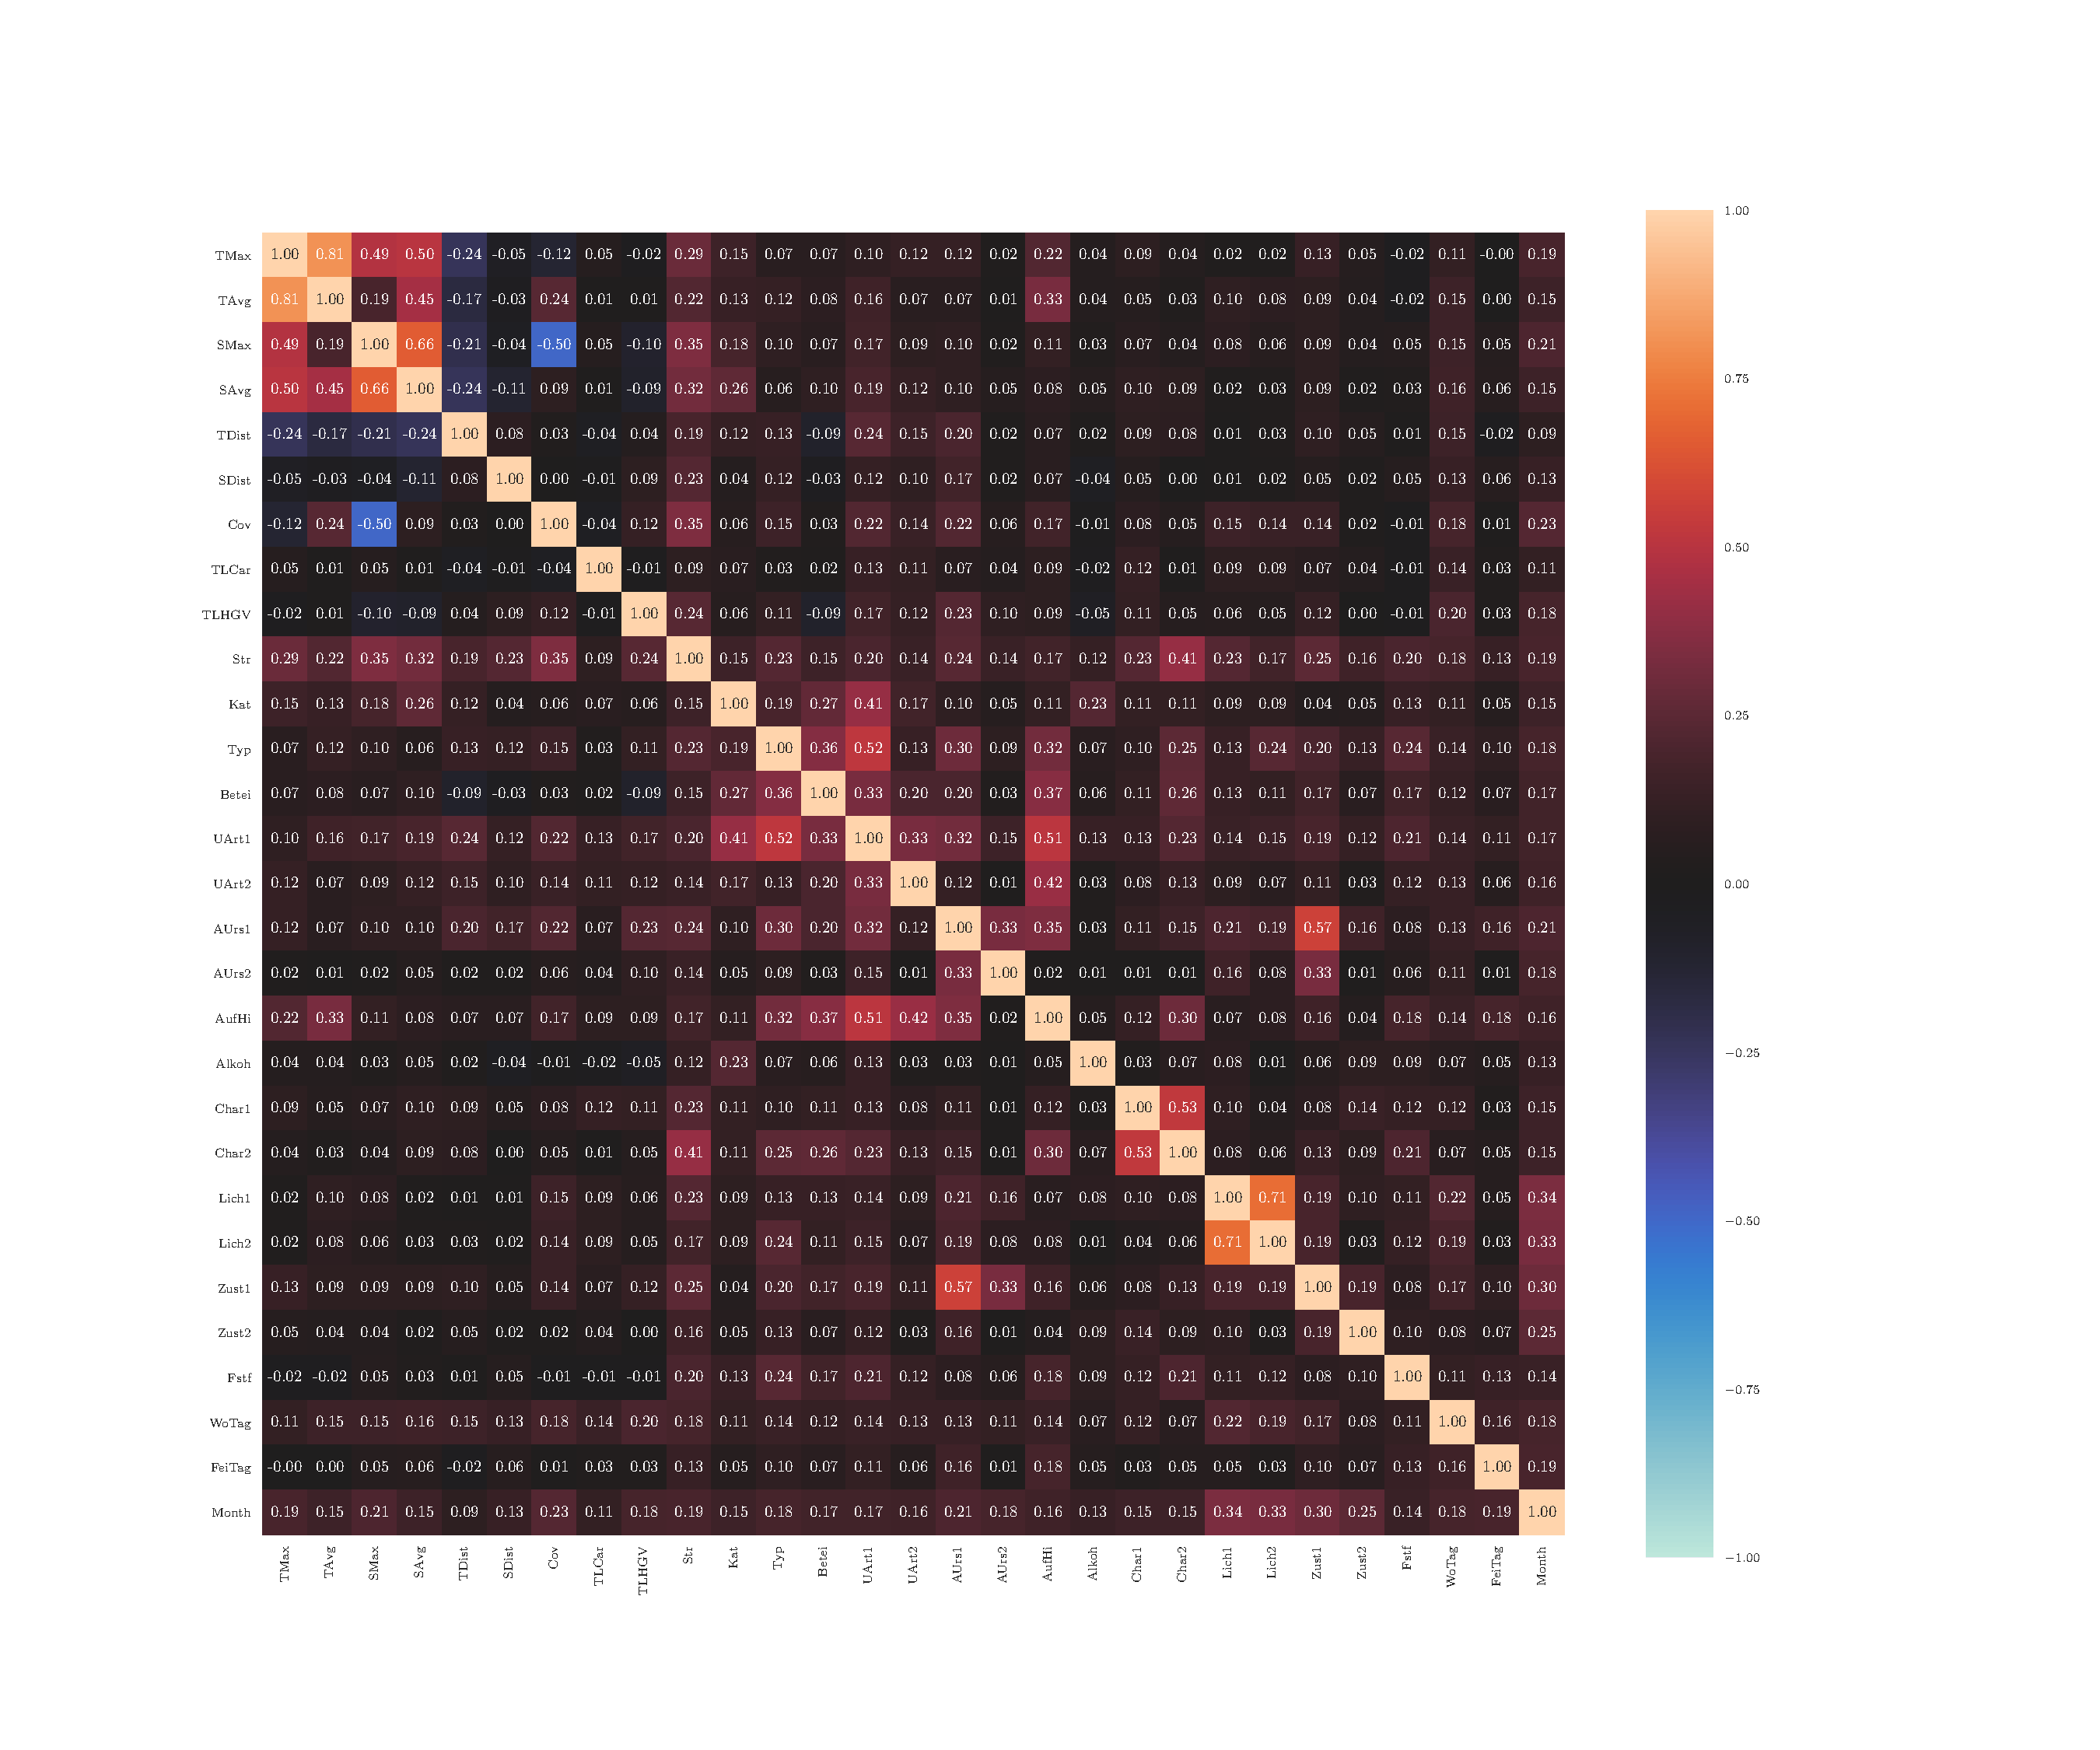
\includegraphics[width=1.4\textwidth, trim=0cm 2.5cm 6cm 3cm]{CorrAnalysis/data/BAYSIS/03_selected_03_endJam/plots/baysis_selected_corr_cramers}%
	}
	\caption{Correlation matrix for congestion-accident matched data classified as \textit{Jam Effector}, with $V$, $\eta$, $\tau$, $r_{pq}$, $r$}
	\label{img:correlation_matrix_selected_effector_cramers}
\end{figure}

% --------------------------
% -------- Strasse ---------
% --------------------------
\centerheading{Strasse}
All relations of \textit{Strasse} - \textit{TMax}, \textit{Strasse} - \textit{TAvg}, \textit{Strasse} - \textit{SMax}, \textit{Strasse} - \textit{SAvg}, \textit{Strasse} - \textit{TDist}, \textit{Strasse} - \textit{SDist}, \textit{Strasse} - \textit{Cov} and \textit{Strasse} - \textit{TLHGV} produce a $p$-value above the $\alpha$-level. The null hypothesizes can't be rejected and there are \textit{no} significant differences between the groups of \textit{Strasse} in these relations.

% ----------------------
% -------- Kat ---------
% ----------------------
\centerheading{Kat}
Both relations of \textit{Kat} - \textit{TMax} and \textit{Kat} - \textit{SAvg} produce a $p$-value above the $\alpha$-level. The null hypothesizes can't be rejected and there are \textit{no} significant differences between the groups of \textit{Kat} in these relations.

% ------------------------
% -------- UArt ---------
% ------------------------
\centerheading{UArt}
All relations of \textit{UArt1} - \textit{TAvg}, \textit{UArt1} - \textit{SAvg}, \textit{UArt1} - \textit{TDist}, \textit{UArt1} - \textit{Cov}, \textit{UArt1} - \textit{TLHGV} and \textit{UArt2} - \textit{TDist} produce a $p$-value above the $\alpha$-level. The null hypothesizes can't be rejected and there are \textit{no} significant differences between the groups of \textit{Strasse} in these relations.

% ------------------------
% -------- AUrs ---------
% ------------------------
\centerheading{AUrs}
This section analyzes the correlated relations of the accident variable \textit{AUrs1}. The correlations of \textit{AUrs1} - \textit{TDist} and \textit{AUrs1} - \textit{TLHGV} produces a $p$-value above the $\alpha$-level of .05 in the Kruskal-Wallis rank sum test. The null hypothesis can't therefore be rejected for these relations and there are no significant groups to identify.

The Kruskal-Wallis rank sum test of \textit{AUrs1} - \textit{SDist} produces a $p$-value of 0.0372, which is below $\alpha=.05$. The null hypothesis can therefore be rejected, which means there is a significant difference between the groups of \textit{Strasse}. To identify the significant groups, a pairwise Wilcoxon $T$-test for \textit{AUrs1} - \textit{TMax} is run, which produces \cref{tbl:wilcoxon_baysis_follower_AUrs1_SDist}. 
\begin{table}[ht]
	\tiny
	\centering
	\begin{tabular}{rrrrrrr}
		\toprule
		& 0 & 72 & 73 & 80 & 82 & 88 \\ 
		\midrule
		72 & 1.00 &  &  &  &  &  \\ 
		73 & 0.10 & 0.35 &  &  &  &  \\ 
		80 & 1.00 &  & 1.00 &  &  &  \\ 
		82 & 1.00 &  & 1.00 &  &  &  \\ 
		88 & 0.40 & 0.04 & 1.00 & 1.00 & 0.55 &  \\ 
		89 & 1.00 &  & 1.00 &  &  & 1.00 \\ 
		\bottomrule
	  \end{tabular}
    \caption{Pairwise Wilcoxon $T$-test for \textit{AUrs1} and \textit{Spatial Distance} (Jam Follower)}
    \label{tbl:wilcoxon_baysis_follower_AUrs1_SDist}
\end{table}
The tables shows that the differences are not group specific, since no groups differs significantly. \todo{Add section of Global and Specific Signifcancy}

The Kruskal-Wallis rank sum test of \textit{AUrs1} - \textit{Cov} produces a $p$-value of 0.0024, which is below $\alpha=.05$. The null hypothesis can therefore be rejected, which means there is a significant difference between the groups of \textit{Strasse}. To identify the significant groups, a pairwise Wilcoxon $T$-test for \textit{AUrs1} - \textit{Cov} is run, which produces \cref{tbl:wilcoxon_baysis_follower_AUrs1_Cov}. 
\begin{table}[ht]
	\tiny
	\centering
	\begin{tabular}{rrrrrrr}
		\toprule
		& 0 & 72 & 73 & 80 & 82 & 88 \\ 
		\midrule
		72 & 0.28 &  &  &  &  &  \\ 
		73 & 1.00 & 1.00 &  &  &  &  \\ 
		80 & 1.00 & 1.00 & 1.00 &  &  &  \\ 
		82 & 1.00 & 1.00 & 1.00 & 1.00 &  &  \\ 
		88 & 0.33 & 0.79 & 0.56 & 1.00 & 1.00 &  \\ 
		89 & 1.00 & 1.00 & 1.00 & 1.00 & 1.00 & 1.00 \\ 
		\bottomrule
	  \end{tabular}
    \caption{Pairwise Wilcoxon $T$-test for \textit{AUrs1} and \textit{Coverage} (Jam Follower)}
    \label{tbl:wilcoxon_baysis_follower_AUrs1_Cov}
\end{table}
The tables shows that the differences are not group specific, since no groups differs significantly. \todo{Add section of Global and Specific Signifcancy}

% ------------------------
% -------- AufHi ---------
% ------------------------
\centerheading{AufHi}
All relations of \textit{AufHi} - \textit{TMax}, \textit{AufHi} - \textit{TAvg} and \textit{AufHi} - \textit{Cov} produce a $p$-value above the $\alpha$-level. The null hypothesizes can't be rejected and there are no significant differences between the groups of \textit{AufHi} in these relations.

% ------------------------
% -------- Lich1 ---------
% ------------------------
\centerheading{Lich}
The relation of \textit{Lich1} - \textit{Cov} produce a $p$-value above $\alpha=.05$ in the Kruskal-Wallis rank sum test. The null hypothesizes can't be rejected and there are \textit{no} significant differences between the groups of \textit{Lich1}.

% ------------------------
% -------- WoTag ---------
% ------------------------
\centerheading{WoTag}

\paragraph{Maximal temporal Extent:}
Kruskal-Wallis chi-squared = 168.61, df = 167, p-value = 0.4506

\paragraph{Maximal spatial Extent:}
Kruskal-Wallis chi-squared = 448.61, df = 425, p-value = 0.2067

\paragraph{Average spatial Extent:}
Kruskal-Wallis chi-squared = 460.72, df = 433, p-value = 0.1723

\paragraph{Temporal Distance}
Kruskal-Wallis chi-squared = 22.628, df = 24, p-value = 0.5418

\paragraph{Coverage}
Kruskal-Wallis chi-squared = 73.906, df = 77, p-value = 0.5788

\paragraph{Time-loss HGV}
Kruskal-Wallis chi-squared = 318.99, df = 293, p-value = 0.1422

% ------------------------
% -------- Month ---------
% ------------------------
\centerheading{Month}

\paragraph{Maximal temporal Extent:}
Kruskal-Wallis chi-squared = 165.89, df = 168, p-value = 0.5316

\paragraph{Average temporal Extent:}
Kruskal-Wallis chi-squared = 182.94, df = 173, p-value = 0.2877

\paragraph{Maximal spatial Extent:}
Kruskal-Wallis chi-squared = 460.69, df = 427, p-value = 0.1258

\paragraph{Coverage}
Kruskal-Wallis chi-squared = 70.545, df = 77, p-value = 0.6849

\paragraph{Time-loss HGV}
Kruskal-Wallis chi-squared = 293.39, df = 293, p-value = 0.4826
\clearpage

% ------------------------
% -------- ArbIS ---------
% ------------------------
\subsection{ArbIS}
\label{analysis_processing_correlation_arbis_matched}
As with the congestion - accident datasets in \cref{analysis_processing_correlation_baysis_matched,analysis_processing_correlation_baysis_initiator,analysis_processing_correlation_baysis_effector,analysis_processing_correlation_baysis_follower} the congestion - roadwork dataset also needs to be analyzed for correlations. The correlation matrix table for the congestion-roadwork dataset (see \cref{tbl:appendix_arbis_correlation_matrix_dataset_cramers}) is visual presented in \cref{img:correlation_matrix_arbis_selected_effector_cramers} showing the the correlation of each variable combination. When visual analyzing \cref{img:correlation_matrix_arbis_selected_effector_cramers} and checking the guidelines for a strong correlation in reference to the applied coefficient (identifiable with \cref{table:appendix_coefficient_matrix_matched}) we get a list of strongly correlated variable combinations (see \cref{tbl:correlation_list_arbis_matched}). Since the focus of the thesis are the correlations between accidents and jams, these are only collected from the bottom-left rectangle of the matrix, where the congestion and accidents variables intersect. Correlations of the kind congestion - congestion or roadwork - roadwork are not considered.
\begin{table}[h!]
	\centering
	\begin{tabular}{c|l|l}  
		Category & Strong \\
		\\[-1em]
		\hline
		\\[-1em]
		Strasse & TMax, TAvg, SMax, SAvg, TDist, SDist, Cov, TLCar, TLHGV \\ 
 		%AnzGesperrtFs & & \\ 
 		%Einzug & & \\
 		%Richtung & & \\
 		%Length & & \\
 		%Duration & & \\
 		Month & TAvg, SMax, SAvg, TDist, SDist, Cov, TLCar \\
	\end{tabular}
  \caption{List of incident variables and their strong/moderated correlated jam variable from the ArbIS matched data}
  \label{tbl:correlation_list_arbis_matched}
\end{table}
As \cref{tbl:correlation_list_arbis_matched} show, only the variables Strasse and Month are correlated with congestion characteristics. Both variables tend to bias an interpretation of congestion characteristics because the 


Next we need to verify that the correlation is significant and what the correlation predicates. Therefore each correlation will be evaluated with the Post Hoc test, defined in \cref{correlation_posthoc}. In the following sections, the correlated relations of the variables in \cref{tbl:correlation_list_arbis_matched} are analyzed and an initial interpretation of each significant correlation is introduced. Groups with an insufficient sample size (see \cref{correlation_uncertainty} are neglected and not shown. The descriptive tables, showing the count ($n$), mean ($\bar{x}$), standard deviation ($\sigma$), median ($\tilde{x}$), $min$, $max$ and range ($\Delta$) therefore only contain groups with significant sample sizes.
\begin{figure}[!ht]
	\centering
	\makebox[\textwidth][c]{%
		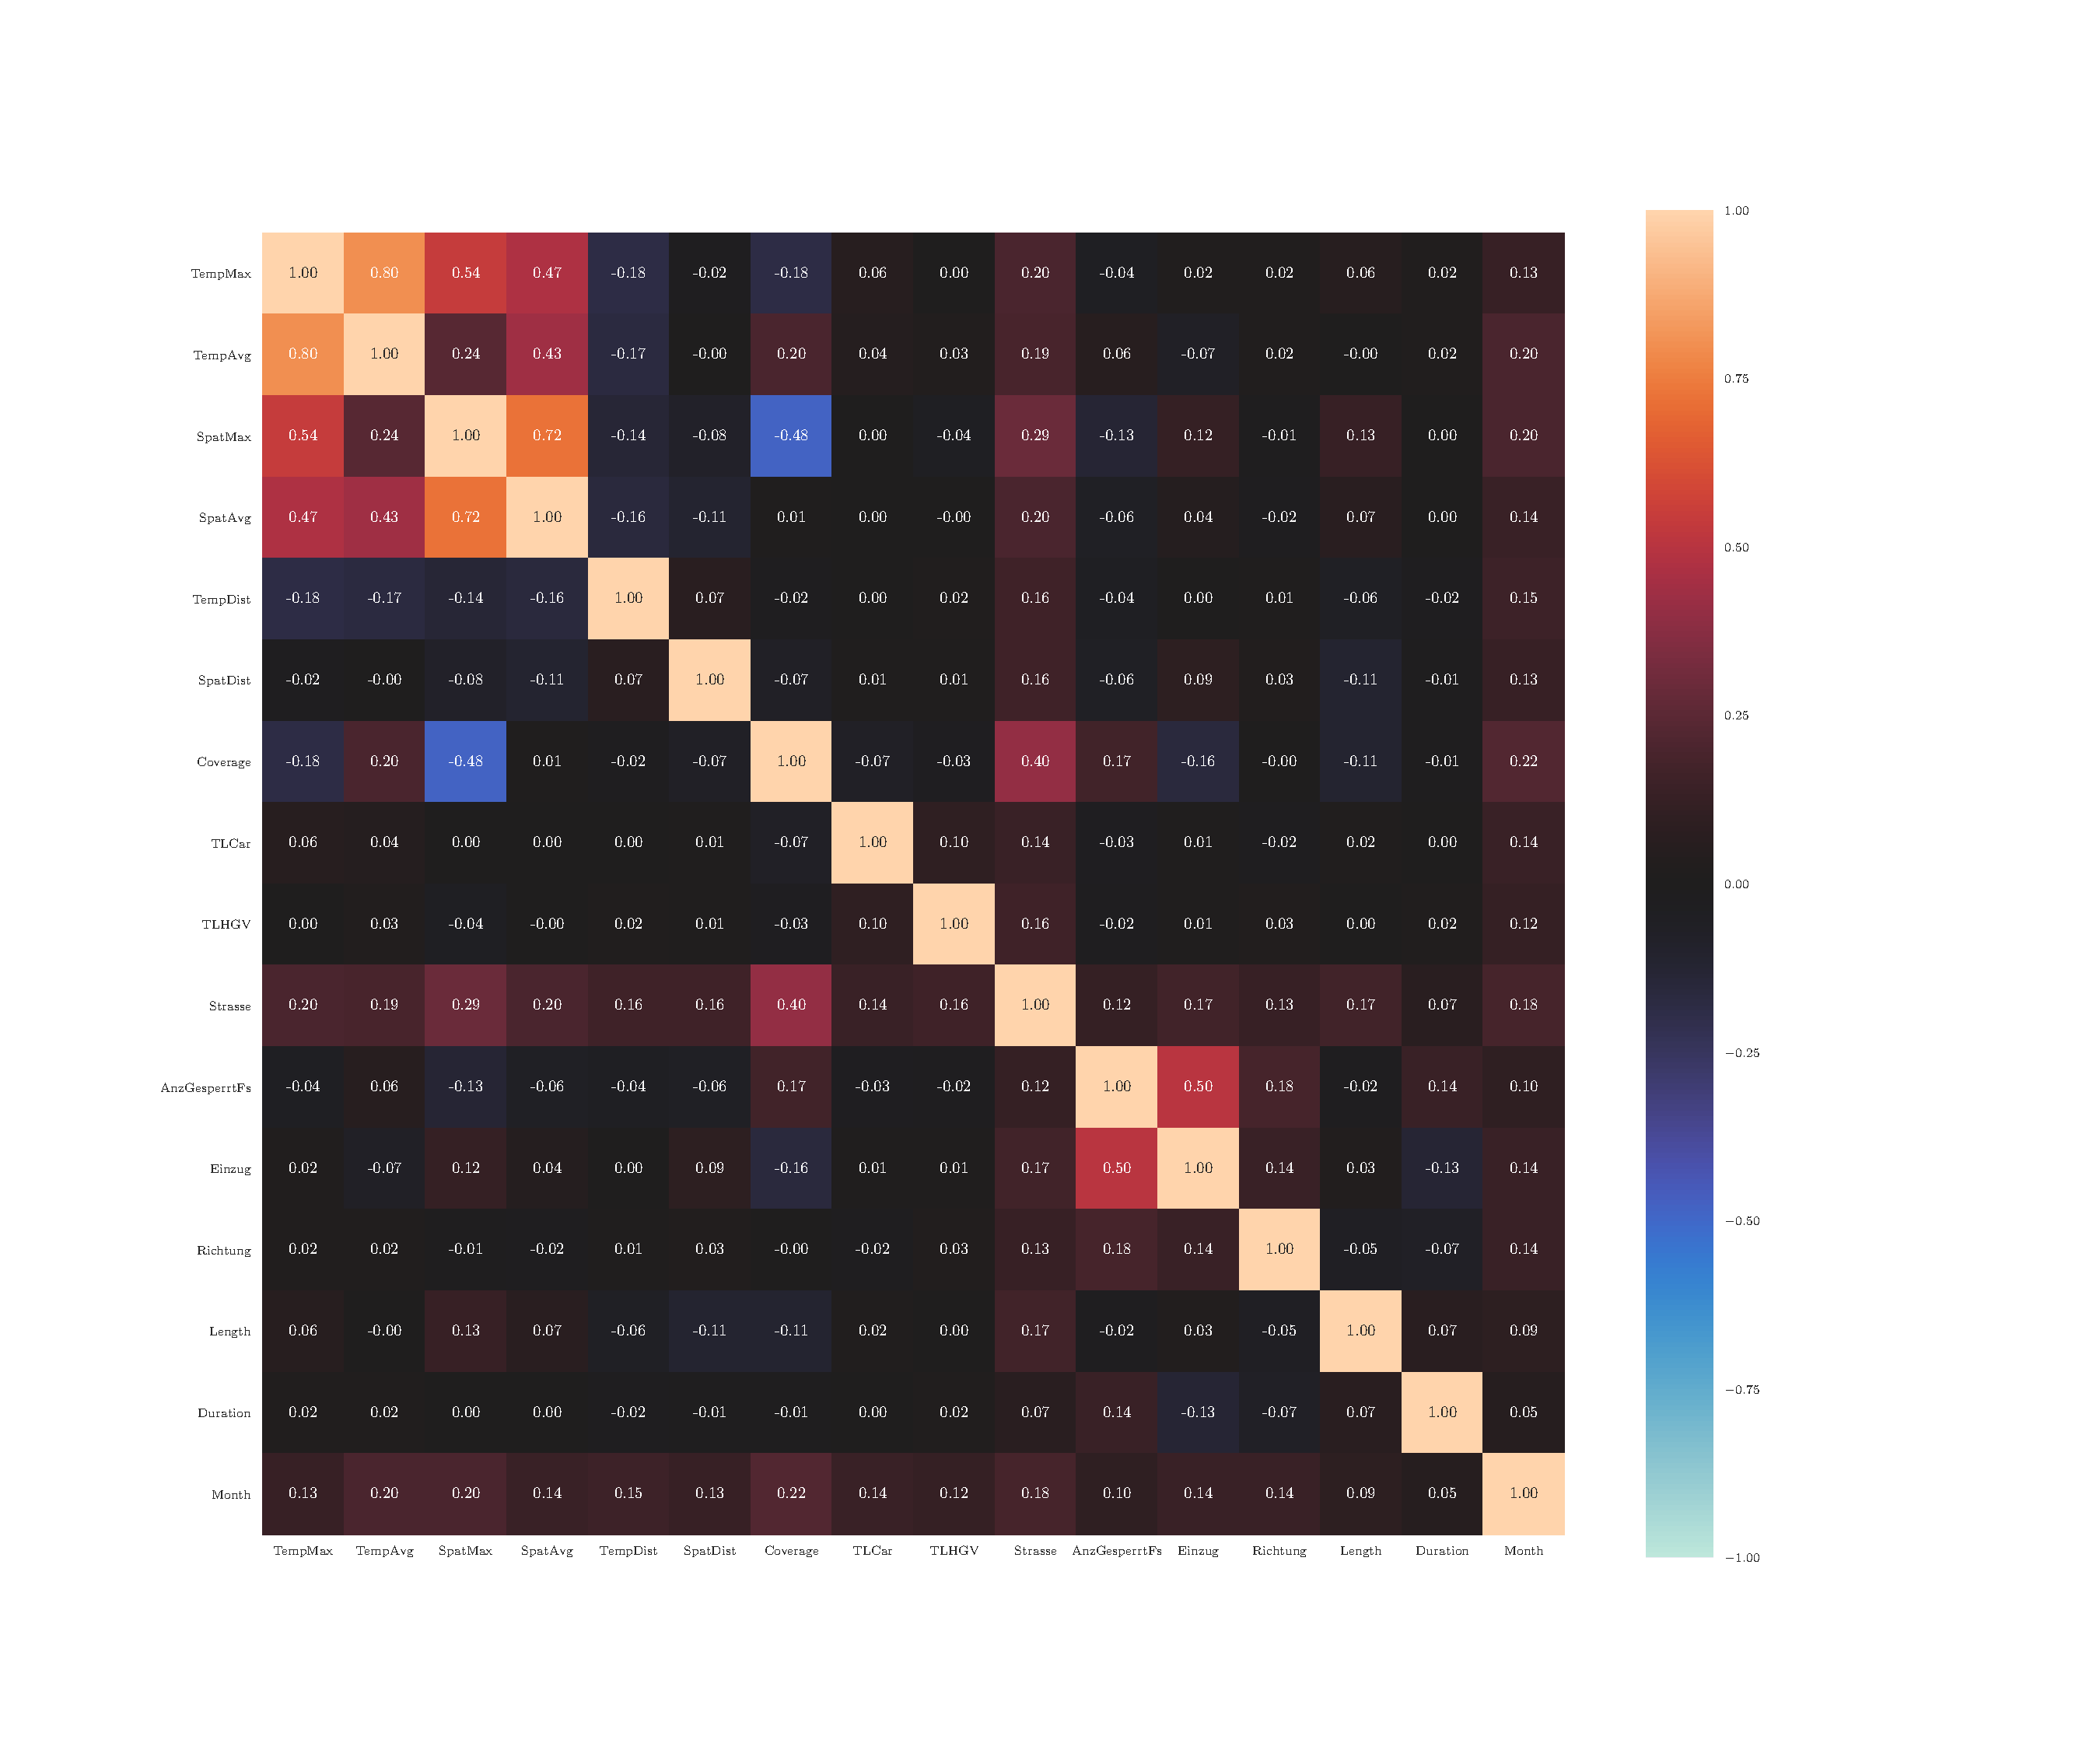
\includegraphics[width=1.4\textwidth, trim=0cm 2.5cm 6cm 3cm]{CorrAnalysis/data/ArbIS/02_matched/plots/arbis_matched_corr_cramers}%
	}
	\caption{Correlation matrix for congestion-roadwork matched data, calculated with $V$, $\eta$, $\tau$, $r_{pq}$, $r$}
	\label{img:correlation_matrix_arbis_selected_effector_cramers}
\end{figure}

% % --------------------------
% % -------- Strasse ---------
% % --------------------------
\centerheading{Strasse}
This section analyzes the correlated relations of the accident variable \textit{Strasse}. The Kruskal-Wallis rank sum test of \textit{Strasse} - \textit{TMax} produces a $p$-value of < 0.0001, which is below $\alpha$. The null hypothesis can therefore be rejected, which means there is a significant difference between the groups of \textit{Strasse}. To identify the significant groups, a pairwise Wilcoxon $T$-test for \textit{Strasse} - \textit{TMax} is run, which produces \cref{tbl:wilcoxon_arbis_matched_Strasse_TMax}. 
\begin{table}[ht!]
	\tiny
	\centering
    \begin{tabular}{rrrrrrrrrrrrrrrrr}
		\toprule
			& A9 & A7 & A70 & A71 & A6 & A73 & A3 & A99 & A96 & A995 & A92 & A72 & A93 & A95 & A94 & A980 \\ 
		\midrule
		% A7   & 1.00 &  &  &  &  &  &  &  &  &  &  &  &  &  &  &  \\ 
		% A70  & 1.00 & 1.00 &  &  &  &  &  &  &  &  &  &  &  &  &  &  \\ 
		% A71  & 1.00 & 1.00 & 1.00 &  &  &  &  &  &  &  &  &  &  &  &  &  \\ 
		% A6   & 1.00 & 1.00 & 1.00 & 1.00 &  &  &  &  &  &  &  &  &  &  &  &  \\ 
		% A73  & 1.00 & 1.00 & 1.00 & 1.00 & 1.00 &  &  &  &  &  &  &  &  &  &  &  \\ 
		A3   & \red{0.00} & \red{0.04} & 1.00 & 1.00 & \red{0.01} & 1.00 &  &  &  &  &  &  &  &  &  &  \\ 
		% A99  & 1.00 & 1.00 & 1.00 & 1.00 & 0.48 & 1.00 & 1.00 &  &  &  &  &  &  &  &  &  \\ 
		A96  & 1.00 & 0.82 & 1.00 & 1.00 & 1.00 & 1.00 & \red{0.00} & \red{0.00} &  &  &  &  &  &  &  &  \\ 
		% A995 & 1.00 & 1.00 & 1.00 & 1.00 & 1.00 & 1.00 & 0.79 & 0.74 & 1.00 &  &  &  &  &  &  &  \\ 
		% A92  & 1.00 & 1.00 & 1.00 & 1.00 & 1.00 & 1.00 & 1.00 & 1.00 & 1.00 & 1.00 &  &  &  &  &  &  \\ 
		% A72  & 1.00 & 1.00 & 1.00 & 1.00 & 1.00 & 1.00 & 1.00 & 1.00 & 1.00 & 1.00 & 1.00 &  &  &  &  &  \\ 
		A93  & \red{0.00} & \red{0.00} & 1.00 & 0.09 & \red{0.00} & \red{0.00} & 1.00 & 1.00 & \red{0.00} & \red{0.00} & \red{0.00} & 1.00 &  &  &  &  \\ 
		% A95  & 1.00 & 1.00 & 1.00 & 1.00 & 1.00 & 1.00 & 1.00 & 1.00 & 1.00 & 1.00 & 1.00 & 1.00 & 1.00 &  &  &  \\ 
		A94  & 1.00 & 1.00 & 1.00 & 1.00 & 0.68 & 1.00 & 1.00 & 1.00 & \red{0.01} & 0.48 & 1.00 & 1.00 & 1.00 & 1.00 &  &  \\ 
		% A980 & 1.00 & 1.00 & 1.00 & 1.00 & 1.00 & 1.00 & 1.00 & 1.00 & 1.00 & 1.00 & 1.00 & 1.00 & 1.00 & 1.00 & 1.00 &  \\ 
		% A45  & 1.00 & 1.00 & 1.00 & 1.00 & 1.00 & 1.00 & 1.00 & 1.00 & 1.00 & 1.00 & 1.00 & 1.00 & 1.00 & 1.00 & 1.00 & 1.00 \\ 
		\bottomrule
	\end{tabular}
	\caption{Pairwise Wilcoxon $T$-test for \textit{Strasse} and \textit{Maximal Temporal Extent}}
	\label{tbl:wilcoxon_arbis_matched_Strasse_TMax}
\end{table}
The table shows, that the groups A3 and A93 differ from group A9, A7 and A6. The A93 also differs from A96, A995 and A92. The A96 differs from A3 and A99.
\begin{table}[ht!]
	\tiny
	\centering
  \begin{tabular}{rrrrrrrrrrrrrr}
    \toprule
    Group & $n$ & $\bar{x}$ & $\sigma$ & $\tilde{x}$ & $min$ & $max$ & $\Delta$ \\
    \midrule
    A9   & 656  & 159.55 & 175.78 & 100.50 & 9   & 1323 & 1314 \\ 
    A7   & 302  & 158.38 & 213.55 & 87.00  & 9   & 1323 & 1314 \\ 
    A70  & 50   & 228.90 & 279.03 & 105.00 & 15  & 963  & 948 \\ 
    A71  & 10   & 83.40  & 72.87  & 48.00  & 36  & 249  & 213 \\ 
    A6   & 198  & 142.24 & 166.46 & 85.50  & 9   & 864  & 855 \\ 
    A73  & 86   & 153.59 & 235.85 & 100.50 & 9   & 1323 & 1314 \\ 
    A3   & 1023 & 233.66 & 279.35 & 123.00 & 9   & 1326 & 1317 \\ 
    A99  & 312  & 158.88 & 155.05 & 135.00 & 9   & 1320 & 1311 \\ 
    A96  & 230  & 105.80 & 95.17  & 75.00  & 9   & 384  & 375 \\ 
    A995 & 14   & 60.00  & 28.70  & 48.00  & 18  & 105  & 87 \\ 
    A92  & 82   & 132.40 & 134.72 & 79.50  & 9   & 768  & 759 \\ 
    A93  & 160  & 157.33 & 55.97  & 189.00 & 9   & 312  & 303 \\  
    A94  & 56   & 179.57 & 124.79 & 165.00 & 15  & 369  & 354 \\ 
    \bottomrule
  \end{tabular}
	\caption{Group descriptives of \textit{Strasse} and \textit{Maximal Temporal Extent}}
	\label{tbl:descriptives_arbis_matched_Strasse_TMax}
	%\vspace{-8mm}
\end{table}
With the descriptives in \cref{tbl:descriptives_arbis_matched_Strasse_TMax} and the named significant differences it can be interpreted that roadworks on the A3 result in 80\,\% longer $\bar{x}$ than on the A9, A7 and A6. The A70 has a similar difference. Roadworks on the A96 and A995 result in significantly shorter $\bar{x}$ than on the A3 and A99.

The Kruskal-Wallis rank sum test of \textit{Strasse} - \textit{TAvg} produces a $p$-value of < 0.0001, which is below $\alpha$. The null hypothesis can therefore be rejected, which means there is a significant difference between the groups of \textit{Strasse}. To identify the significant groups, a pairwise Wilcoxon $T$-test for \textit{Strasse} - \textit{TAvg} is run, which produces \cref{tbl:wilcoxon_arbis_matched_Strasse_TAvg}. 
\begin{table}[ht!]
	\tiny
	\setlength{\tabcolsep}{4pt}
	\centering
  \begin{tabular}{rrrrrrrrrrrrrrrrr}
    \toprule
         & A9 & A7 & A70 & A71 & A6 & A73 & A3 & A99 & A96 & A995 & A92 & A72 & A93 & A95 & A94 & A980 \\ 
    \midrule
    A7   & 1.00 &  &  &  &  &  &  &  &  &  &  &  &  &  &  &  \\ 
    A70  & 1.00 & 1.00 &  &  &  &  &  &  &  &  &  &  &  &  &  &  \\ 
    A71  & 1.00 & 1.00 & 1.00 &  &  &  &  &  &  &  &  &  &  &  &  &  \\ 
    A6   & 1.00 & 1.00 & 1.00 & 1.00 &  &  &  &  &  &  &  &  &  &  &  &  \\ 
    A73  & 1.00 & 1.00 & 1.00 & 1.00 & 1.00 &  &  &  &  &  &  &  &  &  &  &  \\ 
    A3   & 1.00 & 1.00 & 1.00 & 1.00 & 0.69 & 1.00 &  &  &  &  &  &  &  &  &  &  \\ 
    A99  & \red{0.00} & \red{0.00} & 0.08 & 1.00 & 1.00 & 1.00 & \red{0.00} &  &  &  &  &  &  &  &  &  \\ 
    A96  & 1.00 & 1.00 & 1.00 & 1.00 & 1.00 & 1.00 & 1.00 & 0.55 &  &  &  &  &  &  &  &  \\ 
    A995 & 1.00 & 1.00 & 1.00 & 1.00 & 1.00 & 1.00 & 1.00 & 1.00 & 1.00 &  &  &  &  &  &  &  \\ 
    A92  & 1.00 & 1.00 & 1.00 & 1.00 & 1.00 & 1.00 & 1.00 & \red{0.04} & 1.00 & 1.00 &  &  &  &  &  &  \\ 
    A72  & 1.00 & 1.00 & 1.00 & 1.00 & 1.00 & 1.00 & 1.00 & 1.00 & 1.00 & 1.00 & 1.00 &  &  &  &  &  \\ 
    A93  & \red{0.00} & \red{0.00} & 1.00 & 0.24 & \red{0.00} & \red{0.00} & \red{0.00} & \red{0.00} & \red{0.00} & \red{0.00} & \red{0.00} & 1.00 &  &  &  &  \\ 
    A95  & 1.00 & 1.00 & 1.00 & 1.00 & 1.00 & 1.00 & 1.00 & 1.00 & 1.00 & 1.00 & 1.00 & 1.00 & 1.00 &  &  &  \\ 
    A94  & 1.00 & 1.00 & 1.00 & 1.00 & 0.14 & 1.00 & 1.00 & 0.00 & 0.63 & 0.53 & 1.00 & 1.00 & 0.02 & 1.00 &  &  \\ 
    A980 & 1.00 & 1.00 & 1.00 & 1.00 & 1.00 & 1.00 & 1.00 & 1.00 & 1.00 & 1.00 & 1.00 & 1.00 & 1.00 & 1.00 & 1.00 &  \\ 
    A45  & 1.00 & 1.00 & 1.00 & 1.00 & 1.00 & 1.00 & 1.00 & 1.00 & 1.00 & 1.00 & 1.00 & 1.00 & 1.00 & 1.00 & 1.00 & 1.00 \\ 
    \midrule
  \end{tabular}
	\caption{Pairwise Wilcoxon $T$-test for \textit{Strasse} and \textit{Average Temporal Extent}}
	\label{tbl:wilcoxon_arbis_matched_Strasse_TAvg}
\end{table}
The table shows, that the groups A99 and A93 differ from group A9 and A7. The A93 also differs from the A6, A73, A3, A99, A96, A995 and A92. The A92 differs from A99.
\begin{table}[ht!]
	\tiny
	\centering
  \begin{tabular}{rrrrrrrrrrrrrr}
    \toprule
    Group & $n$ & $\bar{x}$ & $\sigma$ & $\tilde{x}$ & $min$ & $max$ & $\Delta$ \\
    \midrule
    A9   & 656  & 85.61  & 100.78 & 42.00  & 5  & 575  & 570 \\ 
    A7   & 302  & 87.76  & 117.13 & 44.50  & 5  & 858  & 853 \\ 
    A70  & 50   & 154.38 & 236.49 & 55.50  & 6  & 966  & 960 \\ 
    A71  & 10   & 64.90  & 71.81  & 38.00  & 18 & 252  & 234 \\ 
    A6   & 198  & 65.60  & 86.36  & 41.00  & 4  & 630  & 626 \\ 
    A73  & 86   & 56.23  & 45.35  & 42.50  & 6  & 190  & 184 \\ 
    A3   & 1023 & 89.94  & 124.69 & 51.00  & 3  & 1326 & 1323 \\ 
    A99  & 312  & 45.38  & 41.73  & 33.00  & 3  & 291  & 288 \\ 
    A96  & 230  & 69.31  & 73.52  & 43.00  & 5  & 290  & 285 \\ 
    A995 & 14   & 37.14  & 23.98  & 23.00  & 8  & 74   & 66 \\ 
    A92  & 82   & 81.83  & 90.35  & 45.50  & 5  & 489  & 484 \\ 
    A93  & 160  & 115.96 & 50.96  & 141.00 & 6  & 199  & 193 \\ 
    A94  & 56   & 84.98  & 64.07  & 70.00  & 6  & 248  & 242 \\ 
    \midrule
  \end{tabular}
	\caption{Group descriptives of \textit{Strasse} and \textit{Average Temporal Extent}}
	\label{tbl:descriptives_arbis_matched_Strasse_TAvg}
	%\vspace{-8mm}
\end{table}
With the descriptives in \cref{tbl:descriptives_arbis_matched_Strasse_TAvg} it can be interpreted that roadworks on the A93 result in sing

The Kruskal-Wallis rank sum test of \textit{Strasse} - \textit{SMax} produces a $p$-value of < 0.0001, which is below $\alpha$. The null hypothesis can therefore be rejected, which means there is a significant difference between the groups of \textit{Strasse}. To identify the significant groups, a pairwise Wilcoxon $T$-test for \textit{Strasse} - \textit{SMax} is run, which produces \cref{tbl:wilcoxon_arbis_matched_Strasse_SMax}. 
\begin{table}[ht!]
	\tiny
	\setlength{\tabcolsep}{4pt}
	\centering
  \begin{tabular}{rrrrrrrrrrrrrrrrr}
    \toprule
         & A9 & A7 & A70 & A71 & A6 & A73 & A3 & A99 & A96 & A995 & A92 & A72 & A93 & A95 & A94 & A980 \\ 
    \hline
    A7   & 0.58 &  &  &  &  &  &  &  &  &  &  &  &  &  &  &  \\ 
    A70  & 1.00 & 1.00 &  &  &  &  &  &  &  &  &  &  &  &  &  &  \\ 
    A71  & 1.00 & 1.00 & 1.00 &  &  &  &  &  &  &  &  &  &  &  &  &  \\ 
    A6   & 1.00 & 1.00 & 1.00 & 1.00 &  &  &  &  &  &  &  &  &  &  &  &  \\ 
    A73  & 1.00 & 1.00 & 1.00 & 1.00 & 1.00 &  &  &  &  &  &  &  &  &  &  &  \\ 
    A3   & 0.00 & 0.00 & 0.00 & 0.52 & 0.01 & 0.05 &  &  &  &  &  &  &  &  &  &  \\ 
    A99  & 0.07 & 0.00 & 0.01 & 0.21 & 0.26 & 0.20 & 1.00 &  &  &  &  &  &  &  &  &  \\ 
    A96  & 0.00 & 0.06 & 1.00 & 1.00 & 0.00 & 1.00 & 0.00 & 0.00 &  &  &  &  &  &  &  &  \\ 
    A995 & 1.00 & 1.00 & 1.00 & 1.00 & 1.00 & 1.00 & 0.11 & 0.03 & 1.00 &  &  &  &  &  &  &  \\ 
    A92  & 1.00 & 1.00 & 1.00 & 1.00 & 1.00 & 1.00 & 0.00 & 0.00 & 0.04 & 1.00 &  &  &  &  &  &  \\ 
    A72  & 1.00 & 1.00 & 1.00 & 1.00 & 1.00 & 1.00 & 1.00 & 1.00 & 1.00 & 0.81 & 1.00 &  &  &  &  &  \\ 
    A93  & 0.00 & 0.00 & 0.02 & 1.00 & 0.00 & 0.00 & 0.00 & 0.00 & 0.00 & 1.00 & 0.00 & 0.73 &  &  &  &  \\ 
    A95  & 1.00 & 1.00 & 1.00 & 1.00 & 1.00 & 1.00 & 1.00 & 1.00 & 1.00 & 1.00 & 1.00 & 1.00 & 1.00 &  &  &  \\ 
    A94  & 1.00 & 1.00 & 1.00 & 1.00 & 1.00 & 1.00 & 0.04 & 0.04 & 0.89 & 1.00 & 1.00 & 1.00 & 0.00 & 1.00 &  &  \\ 
    A980 & 1.00 & 1.00 & 1.00 & 1.00 & 1.00 & 1.00 & 1.00 & 1.00 & 1.00 & 1.00 & 1.00 & 1.00 & 1.00 & 1.00 & 1.00 &  \\ 
    A45  & 1.00 & 1.00 & 1.00 & 1.00 & 1.00 & 1.00 & 1.00 & 1.00 & 1.00 & 1.00 & 1.00 & 1.00 & 1.00 & 1.00 & 1.00 & 1.00 \\ 
    \hline
  \end{tabular}
	\caption{Pairwise Wilcoxon $T$-test for \textit{Strasse} and \textit{Maximal Spatial Extent}}
	\label{tbl:wilcoxon_arbis_matched_Strasse_SMax}
\end{table}
\cref{tbl:wilcoxon_arbis_matched_Strasse_SMax} shows, that the groups A6, A9, A7, A70, A73, A92, A94 and A96 differ from group A3. There is no distinctive general trend.
\begin{table}[ht!]
	\tiny
	\centering
  \begin{tabular}{rrrrrrrrrrrrrr}
    \hline
    & vars & n & mean & sd & median & trimmed & mad & min & max & range & skew & kurtosis & se \\ 
    \hline
    A9   & 1.00 & 656.00 & 8655.57 & 8521.51 & 4778.00 & 6972.99 & 3783.60 & 1035.00 & 49765.00 & 48730.00 & 1.85 & 3.49 & 332.71 \\ 
    A7   & 1.00 & 302.00 & 6238.63 & 4902.30 & 4397.00 & 5486.83 & 2874.76 & 902.00 & 20030.00 & 19128.00 & 1.21 & 0.37 & 282.10 \\ 
    A70  & 1.00 & 50.00 & 5729.56 & 4763.20 & 3224.00 & 4856.50 & 2511.52 & 1365.00 & 20249.00 & 18884.00 & 1.39 & 1.03 & 673.62 \\ 
    A71  & 1.00 & 10.00 & 3899.00 & 2746.84 & 2339.00 & 3336.25 & 391.41 & 2075.00 & 10225.00 & 8150.00 & 1.20 & 0.06 & 868.63 \\ 
    A6   & 1.00 & 198.00 & 8421.67 & 8209.85 & 5690.00 & 6919.39 & 4487.83 & 965.00 & 40033.00 & 39068.00 & 1.83 & 3.14 & 583.45 \\ 
    A73  & 1.00 & 86.00 & 7717.21 & 7747.18 & 4813.00 & 6183.17 & 4233.56 & 1095.00 & 33764.00 & 32669.00 & 1.99 & 3.84 & 835.40 \\ 
    A3   & 1.00 & 1023.00 & 11836.50 & 11045.29 & 7979.00 & 9944.23 & 7856.30 & 1014.00 & 47607.00 & 46593.00 & 1.40 & 1.38 & 345.33 \\ 
    A99  & 1.00 & 312.00 & 9337.49 & 7230.99 & 7978.00 & 8264.88 & 6980.82 & 991.00 & 48987.00 & 47996.00 & 1.78 & 4.68 & 409.37 \\ 
    A96  & 1.00 & 230.00 & 5639.41 & 6034.92 & 3072.00 & 4226.37 & 1856.96 & 951.00 & 27965.00 & 27014.00 & 2.07 & 3.48 & 397.93 \\ 
    A995 & 1.00 & 14.00 & 3618.14 & 1331.10 & 4288.00 & 3684.67 & 796.16 & 1613.00 & 4825.00 & 3212.00 & -0.35 & -1.78 & 355.75 \\ 
    A92  & 1.00 & 82.00 & 5758.10 & 3673.73 & 4544.00 & 5227.71 & 3114.94 & 999.00 & 16931.00 & 15932.00 & 1.22 & 0.92 & 405.70 \\ 
    A93  & 1.00 & 160.00 & 3530.39 & 3718.54 & 1926.00 & 2571.59 & 34.10 & 699.00 & 22528.00 & 21829.00 & 3.21 & 9.95 & 293.98 \\ 
    A94  & 1.00 & 56.00 & 5849.05 & 3394.57 & 5785.00 & 5667.57 & 2513.01 & 1025.00 & 12582.00 & 11557.00 & 0.47 & -0.67 & 453.62 \\ 
    \hline
  \end{tabular}
	\caption{Group descriptives of \textit{Strasse} and \textit{Maximal Spatial Extent}}
	\label{tbl:descriptives_arbis_matched_Strasse_SMax}
	%\vspace{-8mm}
\end{table}
The descriptives in \cref{tbl:descriptives_arbis_matched_Strasse_SMax}

The Kruskal-Wallis rank sum test of \textit{Strasse} - \textit{SAvg} produces a $p$-value of < 0.0001, which is below $\alpha$. The null hypothesis can therefore be rejected, which means there is a significant difference between the groups of \textit{Strasse}. To identify the significant groups, a pairwise Wilcoxon $T$-test for \textit{Strasse} - \textit{SAvg} is run, which produces \cref{tbl:wilcoxon_arbis_matched_Strasse_SAvg}. 
\begin{table}[ht!]
	\tiny
	\setlength{\tabcolsep}{4pt}
	\centering
  \begin{tabular}{rrrrrrrrrrrrrrrrr}
    \hline
         & A9 & A7 & A70 & A71 & A6 & A73 & A3 & A99 & A96 & A995 & A92 & A72 & A93 & A95 & A94 & A980 \\ 
    \hline
    A7   & 0.06 &  &  &  &  &  &  &  &  &  &  &  &  &  &  &  \\ 
    A70  & 1.00 & 1.00 &  &  &  &  &  &  &  &  &  &  &  &  &  &  \\ 
    A71  & 1.00 & 1.00 & 1.00 &  &  &  &  &  &  &  &  &  &  &  &  &  \\ 
    A6   & 1.00 & 1.00 & 1.00 & 1.00 &  &  &  &  &  &  &  &  &  &  &  &  \\ 
    A73  & 0.62 & 1.00 & 1.00 & 1.00 & 1.00 &  &  &  &  &  &  &  &  &  &  &  \\ 
    A3   & 1.00 & 0.00 & 1.00 & 1.00 & 1.00 & 0.02 &  &  &  &  &  &  &  &  &  &  \\ 
    A99  & 0.01 & 1.00 & 1.00 & 1.00 & 0.75 & 1.00 & 0.00 &  &  &  &  &  &  &  &  &  \\ 
    A96  & 0.00 & 1.00 & 1.00 & 1.00 & 0.44 & 1.00 & 0.00 & 1.00 &  &  &  &  &  &  &  &  \\ 
    A995 & 1.00 & 1.00 & 1.00 & 1.00 & 1.00 & 1.00 & 1.00 & 1.00 & 1.00 &  &  &  &  &  &  &  \\ 
    A92  & 1.00 & 0.62 & 1.00 & 1.00 & 1.00 & 0.73 & 1.00 & 0.10 & 0.14 & 1.00 &  &  &  &  &  &  \\ 
    A72  & 1.00 & 1.00 & 1.00 & 1.00 & 1.00 & 1.00 & 1.00 & 1.00 & 1.00 & 1.00 & 1.00 &  &  &  &  &  \\ 
    A93  & 0.00 & 0.13 & 1.00 & 1.00 & 0.00 & 1.00 & 0.00 & 0.11 & 1.00 & 1.00 & 0.00 & 1.00 &  &  &  &  \\ 
    A95  & 1.00 & 1.00 & 1.00 & 1.00 & 1.00 & 1.00 & 1.00 & 1.00 & 1.00 & 1.00 & 1.00 & 1.00 & 1.00 &  &  &  \\ 
    A94  & 1.00 & 1.00 & 1.00 & 1.00 & 1.00 & 1.00 & 1.00 & 1.00 & 1.00 & 1.00 & 1.00 & 1.00 & 1.00 & 1.00 &  &  \\ 
    A980 & 1.00 & 1.00 & 1.00 & 1.00 & 1.00 & 1.00 & 1.00 & 1.00 & 1.00 & 1.00 & 1.00 & 1.00 & 1.00 & 1.00 & 1.00 &  \\ 
    A45  & 1.00 & 1.00 & 1.00 & 1.00 & 1.00 & 1.00 & 1.00 & 1.00 & 1.00 & 1.00 & 1.00 & 1.00 & 1.00 & 1.00 & 1.00 & 1.00 \\ 
    \hline
  \end{tabular}
	\caption{Pairwise Wilcoxon $T$-test for \textit{Strasse} and \textit{Average Spatial Extent}}
	\label{tbl:wilcoxon_arbis_matched_Strasse_SAvg}
\end{table}
\cref{tbl:wilcoxon_arbis_matched_Strasse_SAvg} shows, that the groups A6, A9, A7, A70, A73, A92, A94 and A96 differ from group A3. There is no distinctive general trend.
\begin{table}[ht!]
	\tiny
	\centering
  \begin{tabular}{rrrrrrrrrrrrrr}
    \hline
    & vars & n & mean & sd & median & trimmed & mad & min & max & range & skew & kurtosis & se \\ 
    \hline
    A9   & 1.00 & 656.00 & 3537.87 & 3014.80 & 2388.50 & 2920.30 & 1381.78 & 697.00 & 14785.00 & 14088.00 & 1.76 & 2.51 & 117.71 \\ 
    A7   & 1.00 & 302.00 & 2917.97 & 2988.99 & 2113.50 & 2271.17 & 1127.52 & 284.00 & 15602.00 & 15318.00 & 3.08 & 9.64 & 172.00 \\ 
    A70  & 1.00 & 50.00 & 3170.10 & 3033.98 & 1816.00 & 2516.70 & 962.21 & 532.00 & 12543.00 & 12011.00 & 1.72 & 1.88 & 429.07 \\ 
    A71  & 1.00 & 10.00 & 2572.50 & 3027.05 & 1323.00 & 1812.25 & 690.89 & 802.00 & 10425.00 & 9623.00 & 1.73 & 1.62 & 957.24 \\ 
    A6   & 1.00 & 198.00 & 3189.79 & 2385.78 & 2267.00 & 2780.79 & 1272.07 & 458.00 & 14150.00 & 13692.00 & 1.63 & 2.60 & 169.55 \\ 
    A73  & 1.00 & 86.00 & 2508.40 & 1834.03 & 2006.00 & 2228.70 & 1316.55 & 419.00 & 10039.00 & 9620.00 & 1.86 & 4.15 & 197.77 \\ 
    A3   & 1.00 & 1023.00 & 3733.90 & 2979.43 & 2835.00 & 3227.67 & 2269.86 & 355.00 & 15054.00 & 14699.00 & 1.54 & 2.09 & 93.15 \\ 
    A99  & 1.00 & 312.00 & 2381.29 & 1265.40 & 1974.00 & 2225.76 & 1073.40 & 502.00 & 5931.00 & 5429.00 & 1.00 & 0.27 & 71.64 \\ 
    A96  & 1.00 & 230.00 & 2488.22 & 1790.94 & 2160.00 & 2144.86 & 1068.21 & 404.00 & 9767.00 & 9363.00 & 2.10 & 4.77 & 118.09 \\ 
    A995 & 1.00 & 14.00 & 1976.93 & 1044.51 & 1950.00 & 1992.67 & 1714.63 & 569.00 & 3196.00 & 2627.00 & 0.06 & -1.72 & 279.16 \\ 
    A92  & 1.00 & 82.00 & 3360.88 & 2294.30 & 2882.00 & 3040.65 & 1786.53 & 457.00 & 11703.00 & 11246.00 & 1.27 & 1.23 & 253.36 \\ 
    A93  & 1.00 & 160.00 & 2243.26 & 2065.34 & 1575.00 & 1749.74 & 449.23 & 461.00 & 11161.00 & 10700.00 & 3.42 & 11.30 & 163.28 \\  
    A94  & 1.00 & 56.00 & 2557.62 & 1655.86 & 2551.00 & 2354.04 & 1104.54 & 506.00 & 6393.00 & 5887.00 & 1.06 & 0.54 & 221.27 \\ 
    \hline
  \end{tabular}
	\caption{Group descriptives of \textit{Strasse} and \textit{Average Spatial Extent}}
	\label{tbl:descriptives_arbis_matched_Strasse_SAvg}
	%\vspace{-8mm}
\end{table}
The descriptives in \cref{tbl:descriptives_arbis_matched_Strasse_SAvg}

The Kruskal-Wallis rank sum test of \textit{Strasse} - \textit{TDist} produces a $p$-value of < 0.0001, which is below $\alpha$. The null hypothesis can therefore be rejected, which means there is a significant difference between the groups of \textit{Strasse}. To identify the significant groups, a pairwise Wilcoxon $T$-test for \textit{Strasse} - \textit{TDist} is run, which produces \cref{tbl:wilcoxon_arbis_matched_Strasse_TDist}. 
\begin{table}[ht!]
	\tiny
	\setlength{\tabcolsep}{4pt}
	\centering
  \begin{tabular}{rrrrrrrrrrrrrrrrr}
    \hline
         & A9 & A7 & A70 & A71 & A6 & A73 & A3 & A99 & A96 & A995 & A92 & A72 & A93 & A95 & A94 & A980 \\ 
    \hline
    A7   & 0.00 &  &  &  &  &  &  &  &  &  &  &  &  &  &  &  \\ 
    A70  & 0.57 & 1.00 &  &  &  &  &  &  &  &  &  &  &  &  &  &  \\ 
    A71  & 1.00 & 1.00 & 1.00 &  &  &  &  &  &  &  &  &  &  &  &  &  \\ 
    A6   & 0.10 & 1.00 & 1.00 & 1.00 &  &  &  &  &  &  &  &  &  &  &  &  \\ 
    A73  & 1.00 & 1.00 & 1.00 & 1.00 & 1.00 &  &  &  &  &  &  &  &  &  &  &  \\ 
    A3   & 0.00 & 1.00 & 1.00 & 1.00 & 1.00 & 0.85 &  &  &  &  &  &  &  &  &  &  \\ 
    A99  & 0.38 & 1.00 & 1.00 & 1.00 & 1.00 & 1.00 & 0.26 &  &  &  &  &  &  &  &  &  \\ 
    A96  & 1.00 & 1.00 & 1.00 & 1.00 & 1.00 & 1.00 & 0.03 & 1.00 &  &  &  &  &  &  &  &  \\ 
    A995 & 1.00 & 1.00 & 1.00 & 1.00 & 1.00 & 1.00 & 1.00 & 1.00 & 1.00 &  &  &  &  &  &  &  \\ 
    A92  & 0.04 & 1.00 & 1.00 & 1.00 & 1.00 & 1.00 & 1.00 & 1.00 & 1.00 & 1.00 &  &  &  &  &  &  \\ 
    A72  & 1.00 & 1.00 & 1.00 & 1.00 & 1.00 & 1.00 & 1.00 & 1.00 & 1.00 & 1.00 & 1.00 &  &  &  &  &  \\ 
    A93  & 0.63 & 1.00 & 1.00 & 1.00 & 1.00 & 1.00 & 1.00 & 1.00 & 1.00 & 1.00 & 1.00 & 1.00 &  &  &  &  \\ 
    A95  & 1.00 & 1.00 & 1.00 & 1.00 & 1.00 & 1.00 & 1.00 & 1.00 & 1.00 & 1.00 & 1.00 &  & 1.00 &  &  &  \\ 
    A94  & 1.00 & 1.00 & 1.00 & 1.00 & 1.00 & 1.00 & 1.00 & 1.00 & 1.00 & 1.00 & 1.00 & 1.00 & 1.00 & 1.00 &  &  \\ 
    A980 & 1.00 & 1.00 & 1.00 & 1.00 & 1.00 & 1.00 & 1.00 & 1.00 & 1.00 & 1.00 & 1.00 &  & 1.00 &  & 1.00 &  \\ 
    A45  & 1.00 & 1.00 & 1.00 & 1.00 & 1.00 & 1.00 & 1.00 & 1.00 & 1.00 & 1.00 & 1.00 &  & 1.00 &  & 1.00 &  \\ 
    \hline
  \end{tabular}
	\caption{Pairwise Wilcoxon $T$-test for \textit{Strasse} and \textit{Temporal Distance}}
	\label{tbl:wilcoxon_arbis_matched_Strasse_TDist}
\end{table}
\cref{tbl:wilcoxon_arbis_matched_Strasse_TDist} shows, that the groups A6, A9, A7, A70, A73, A92, A94 and A96 differ from group A3. There is no distinctive general trend.
\begin{table}[ht!]
	\tiny
	\centering
  \begin{tabular}{rrrrrrrrrrrrrr}
    \hline
    & vars & n & mean & sd & median & trimmed & mad & min & max & range & skew & kurtosis & se \\ 
    \hline
    A9   & 1.00 & 656.00 & 4.12 & 7.16 & 0.00 & 2.56 & 0.00 & 0.00 & 24.00 & 24.00 & 1.51 & 0.78 & 0.28 \\ 
    A7   & 1.00 & 302.00 & 2.10 & 5.21 & 0.00 & 0.60 & 0.00 & 0.00 & 24.00 & 24.00 & 2.53 & 5.41 & 0.30 \\ 
    A70  & 1.00 & 50.00 & 1.64 & 5.20 & 0.00 & 0.07 & 0.00 & 0.00 & 23.00 & 23.00 & 3.03 & 7.81 & 0.73 \\ 
    A71  & 1.00 & 10.00 & 3.40 & 4.74 & 0.00 & 2.62 & 0.00 & 0.00 & 13.00 & 13.00 & 0.76 & -1.03 & 1.50 \\ 
    A6   & 1.00 & 198.00 & 2.09 & 5.07 & 0.00 & 0.66 & 0.00 & 0.00 & 23.00 & 23.00 & 2.58 & 5.77 & 0.36 \\ 
    A73  & 1.00 & 86.00 & 3.16 & 6.33 & 0.00 & 1.61 & 0.00 & 0.00 & 24.00 & 24.00 & 1.90 & 2.37 & 0.68 \\ 
    A3   & 1.00 & 1023.00 & 1.81 & 4.92 & 0.00 & 0.35 & 0.00 & 0.00 & 24.00 & 24.00 & 2.84 & 7.18 & 0.15 \\ 
    A99  & 1.00 & 312.00 & 2.72 & 5.91 & 0.00 & 1.13 & 0.00 & 0.00 & 24.00 & 24.00 & 2.18 & 3.64 & 0.33 \\ 
    A96  & 1.00 & 230.00 & 3.09 & 6.17 & 0.00 & 1.56 & 0.00 & 0.00 & 24.00 & 24.00 & 1.84 & 2.08 & 0.41 \\ 
    A995 & 1.00 & 14.00 & 1.64 & 6.15 & 0.00 & 0.00 & 0.00 & 0.00 & 23.00 & 23.00 & 2.98 & 7.41 & 1.64 \\ 
    A92  & 1.00 & 82.00 & 1.20 & 3.85 & 0.00 & 0.08 & 0.00 & 0.00 & 22.00 & 22.00 & 3.58 & 12.88 & 0.43 \\ 
    A93  & 1.00 & 160.00 & 2.39 & 5.50 & 0.00 & 0.86 & 0.00 & 0.00 & 23.00 & 23.00 & 2.22 & 3.65 & 0.43 \\ 
    A94  & 1.00 & 56.00 & 2.18 & 5.06 & 0.00 & 0.96 & 0.00 & 0.00 & 23.00 & 23.00 & 2.30 & 4.61 & 0.68 \\ 
    \hline
  \end{tabular}
	\caption{Group descriptives of \textit{Strasse} and \textit{Temporal Distance}}
	\label{tbl:descriptives_arbis_matched_Strasse_TDist}
	%\vspace{-8mm}
\end{table}
The descriptives in \cref{tbl:descriptives_arbis_matched_Strasse_TDist}

The Kruskal-Wallis rank sum test of \textit{Strasse} - \textit{SDist} produces a $p$-value of < 0.0001, which is below $\alpha$. The null hypothesis can therefore be rejected, which means there is a significant difference between the groups of \textit{Strasse}. To identify the significant groups, a pairwise Wilcoxon $T$-test for \textit{Strasse} - \textit{SDist} is run, which produces \cref{tbl:wilcoxon_arbis_matched_Strasse_SDist}. 
\begin{table}[ht!]
	\tiny
	\setlength{\tabcolsep}{4pt}
	\centering
  \begin{tabular}{rrrrrrrrrrrrrrrrr}
    \hline
         & A9 & A7 & A70 & A71 & A6 & A73 & A3 & A99 & A96 & A995 & A92 & A72 & A93 & A95 & A94 & A980 \\ 
    \hline
    A7   & 0.62 &  &  &  &  &  &  &  &  &  &  &  &  &  &  &  \\ 
    A70  & 1.00 & 1.00 &  &  &  &  &  &  &  &  &  &  &  &  &  &  \\ 
    A71  & 1.00 & 1.00 & 1.00 &  &  &  &  &  &  &  &  &  &  &  &  &  \\ 
    A6   & 1.00 & 1.00 & 1.00 & 1.00 &  &  &  &  &  &  &  &  &  &  &  &  \\ 
    A73  & 0.03 & 1.00 & 1.00 & 1.00 & 0.89 &  &  &  &  &  &  &  &  &  &  &  \\ 
    A3   & 1.00 & 1.00 & 1.00 & 1.00 & 1.00 & 0.33 &  &  &  &  &  &  &  &  &  &  \\ 
    A99  & 1.00 & 0.61 & 1.00 & 1.00 & 1.00 & 0.03 & 1.00 &  &  &  &  &  &  &  &  &  \\ 
    A96  & 1.00 & 1.00 & 1.00 & 1.00 & 1.00 & 1.00 & 1.00 & 1.00 &  &  &  &  &  &  &  &  \\ 
    A995 & 1.00 & 1.00 & 1.00 & 1.00 & 1.00 & 1.00 & 1.00 & 1.00 & 1.00 &  &  &  &  &  &  &  \\ 
    A92  & 1.00 & 1.00 & 1.00 & 1.00 & 1.00 & 1.00 & 1.00 & 1.00 & 1.00 & 1.00 &  &  &  &  &  &  \\ 
    A72  & 1.00 & 1.00 & 1.00 & 1.00 & 1.00 & 1.00 & 1.00 & 1.00 & 1.00 & 1.00 & 1.00 &  &  &  &  &  \\ 
    A93  & 0.00 & 0.05 & 1.00 & 1.00 & 0.01 & 1.00 & 0.00 & 0.00 & 0.06 & 0.16 & 0.12 & 1.00 &  &  &  &  \\ 
    A95  & 1.00 & 1.00 & 1.00 & 1.00 & 1.00 & 1.00 & 1.00 & 1.00 & 1.00 & 1.00 & 1.00 &  & 1.00 &  &  &  \\ 
    A94  & 1.00 & 0.09 & 0.72 & 1.00 & 0.76 & 0.00 & 0.40 & 1.00 & 0.30 & 1.00 & 1.00 & 1.00 & 0.00 & 1.00 &  &  \\ 
    A980 & 1.00 & 1.00 & 1.00 & 1.00 & 1.00 & 1.00 & 1.00 & 1.00 & 1.00 & 1.00 & 1.00 &  & 1.00 &  & 1.00 &  \\ 
    A45  & 1.00 & 1.00 & 1.00 & 1.00 & 1.00 & 1.00 & 1.00 & 1.00 & 1.00 & 1.00 & 1.00 & 1.00 & 1.00 & 1.00 & 1.00 & 1.00 \\ 
    \hline
  \end{tabular}
	\caption{Pairwise Wilcoxon $T$-test for \textit{Strasse} and \textit{Spatial Distance}}
	\label{tbl:wilcoxon_arbis_matched_Strasse_SDist}
\end{table}
\cref{tbl:wilcoxon_arbis_matched_Strasse_SDist} shows, that the groups A6, A9, A7, A70, A73, A92, A94 and A96 differ from group A3. There is no distinctive general trend.
\begin{table}[ht!]
	\tiny
	\centering
  \begin{tabular}{rrrrrrrrrrrrrr}
    \hline
    & vars & n & mean & sd & median & trimmed & mad & min & max & range & skew & kurtosis & se \\ 
    \hline
    A9   & 1.00 & 656.00 & 216.54 & 466.13 & 0.00 & 94.31 & 0.00 & 0.00 & 1988.00 & 1988.00 & 2.31 & 4.66 & 18.20 \\ 
    A7   & 1.00 & 302.00 & 106.12 & 329.01 & 0.00 & 8.36 & 0.00 & 0.00 & 1882.00 & 1882.00 & 3.41 & 11.11 & 18.93 \\ 
    A70  & 1.00 & 50.00 & 72.94 & 257.26 & 0.00 & 0.93 & 0.00 & 0.00 & 1253.00 & 1253.00 & 3.54 & 11.42 & 36.38 \\ 
    A71  & 1.00 & 10.00 & 25.80 & 81.59 & 0.00 & 0.00 & 0.00 & 0.00 & 258.00 & 258.00 & 2.28 & 3.57 & 25.80 \\ 
    A6   & 1.00 & 198.00 & 130.20 & 379.68 & 0.00 & 20.11 & 0.00 & 0.00 & 1968.00 & 1968.00 & 3.24 & 9.77 & 26.98 \\ 
    A73  & 1.00 & 86.00 & 49.74 & 245.74 & 0.00 & 0.00 & 0.00 & 0.00 & 1924.00 & 1924.00 & 6.01 & 39.17 & 26.50 \\ 
    A3   & 1.00 & 1023.00 & 137.75 & 381.13 & 0.00 & 24.19 & 0.00 & 0.00 & 1979.00 & 1979.00 & 3.10 & 8.91 & 11.92 \\ 
    A99  & 1.00 & 312.00 & 260.51 & 542.02 & 0.00 & 122.26 & 0.00 & 0.00 & 1977.00 & 1977.00 & 1.90 & 2.07 & 30.69 \\ 
    A96  & 1.00 & 230.00 & 146.79 & 395.78 & 0.00 & 25.03 & 0.00 & 0.00 & 1958.00 & 1958.00 & 2.80 & 6.83 & 26.10 \\ 
    A995 & 1.00 & 14.00 & 288.29 & 545.94 & 0.00 & 190.58 & 0.00 & 0.00 & 1749.00 & 1749.00 & 1.55 & 1.10 & 145.91 \\ 
    A92  & 1.00 & 82.00 & 96.22 & 295.14 & 0.00 & 18.50 & 0.00 & 0.00 & 1626.00 & 1626.00 & 3.90 & 15.67 & 32.59 \\ 
    A93  & 1.00 & 160.00 & 34.58 & 189.72 & 0.00 & 0.00 & 0.00 & 0.00 & 1769.00 & 1769.00 & 6.67 & 49.58 & 15.00 \\ 
    A94  & 1.00 & 56.00 & 327.38 & 606.32 & 0.00 & 198.54 & 0.00 & 0.00 & 1983.00 & 1983.00 & 1.66 & 1.29 & 81.02 \\ 
    \hline
  \end{tabular}
	\caption{Group descriptives of \textit{Strasse} and \textit{Spatial Distance}}
	\label{tbl:descriptives_arbis_matched_Strasse_SDist}
	%\vspace{-8mm}
\end{table}
The descriptives in \cref{tbl:descriptives_arbis_matched_Strasse_SDist}

The Kruskal-Wallis rank sum test of \textit{Strasse} - \textit{Cov} produces a $p$-value of < 0.0001, which is below $\alpha$. The null hypothesis can therefore be rejected, which means there is a significant difference between the groups of \textit{Strasse}. To identify the significant groups, a pairwise Wilcoxon $T$-test for \textit{Strasse} - \textit{Cov} is run, which produces \cref{tbl:wilcoxon_arbis_matched_Strasse_Cov}. 
\begin{table}[ht!]
	\tiny
	\setlength{\tabcolsep}{4pt}
	\centering
  \begin{tabular}{rrrrrrrrrrrrrrrrr}
    \hline
         & A9 & A7 & A70 & A71 & A6 & A73 & A3 & A99 & A96 & A995 & A92 & A72 & A93 & A95 & A94 & A980 \\ 
    \hline
    A7   & 0.07 &  &  &  &  &  &  &  &  &  &  &  &  &  &  &  \\ 
    A70  & 0.01 & 1.00 &  &  &  &  &  &  &  &  &  &  &  &  &  &  \\ 
    A71  & 1.00 & 1.00 & 1.00 &  &  &  &  &  &  &  &  &  &  &  &  &  \\ 
    A6   & 1.00 & 1.00 & 1.00 & 1.00 &  &  &  &  &  &  &  &  &  &  &  &  \\ 
    A73  & 1.00 & 1.00 & 1.00 & 1.00 & 1.00 &  &  &  &  &  &  &  &  &  &  &  \\ 
    A3   & 0.00 & 0.00 & 0.00 & 1.00 & 0.01 & 1.00 &  &  &  &  &  &  &  &  &  &  \\ 
    A99  & 0.00 & 0.00 & 0.00 & 0.15 & 0.00 & 0.00 & 0.00 &  &  &  &  &  &  &  &  &  \\ 
    A96  & 0.00 & 0.18 & 1.00 & 1.00 & 0.00 & 0.00 & 0.00 & 0.00 &  &  &  &  &  &  &  &  \\ 
    A995 & 1.00 & 1.00 & 1.00 & 1.00 & 1.00 & 1.00 & 1.00 & 0.02 & 1.00 &  &  &  &  &  &  &  \\ 
    A92  & 0.00 & 1.00 & 1.00 & 1.00 & 0.04 & 0.05 & 0.00 & 0.00 & 1.00 & 1.00 &  &  &  &  &  &  \\ 
    A72  & 1.00 & 1.00 & 1.00 & 1.00 & 1.00 & 1.00 & 1.00 & 1.00 & 1.00 & 1.00 & 1.00 &  &  &  &  &  \\ 
    A93  & 0.00 & 0.00 & 0.00 & 1.00 & 0.00 & 0.00 & 0.00 & 0.00 & 0.02 & 0.01 & 0.00 & 1.00 &  &  &  &  \\ 
    A95  & 1.00 & 1.00 & 1.00 & 1.00 & 1.00 & 1.00 & 1.00 & 1.00 & 1.00 & 1.00 & 1.00 & 1.00 & 1.00 &  &  &  \\ 
    A94  & 1.00 & 1.00 & 1.00 & 1.00 & 1.00 & 1.00 & 1.00 & 0.00 & 0.36 & 1.00 & 1.00 & 1.00 & 0.00 & 1.00 &  &  \\ 
    A980 & 1.00 & 1.00 & 1.00 & 1.00 & 1.00 & 1.00 & 1.00 & 1.00 & 1.00 & 1.00 & 1.00 & 1.00 & 1.00 & 1.00 & 1.00 &  \\ 
    A45  & 1.00 & 1.00 & 1.00 & 1.00 & 1.00 & 1.00 & 1.00 & 1.00 & 1.00 & 1.00 & 1.00 & 1.00 & 1.00 & 1.00 & 1.00 & 1.00 \\ 
    \hline
  \end{tabular}
	\caption{Pairwise Wilcoxon $T$-test for \textit{Strasse} and \textit{Coverage}}
	\label{tbl:wilcoxon_arbis_matched_Strasse_Cov}
\end{table}
\cref{tbl:wilcoxon_arbis_matched_Strasse_Cov} shows, that the groups A6, A9, A7, A70, A73, A92, A94 and A96 differ from group A3. There is no distinctive general trend.
\begin{table}[ht!]
	\tiny
	\centering
  \begin{tabular}{rrrrrrrrrrrrrr}
    \hline
    & vars & n & mean & sd & median & trimmed & mad & min & max & range & skew & kurtosis & se \\ 
    \hline
    A9   & 1.00 & 656.00 & 45.42 & 16.80 & 47.00 & 44.30 & 17.79 & 7.00 & 100.00 & 93.00 & 0.56 & 0.05 & 0.66 \\ 
    A7   & 1.00 & 302.00 & 51.75 & 26.20 & 53.00 & 50.81 & 29.65 & 6.00 & 100.00 & 94.00 & 0.15 & -0.92 & 1.51 \\ 
    A70  & 1.00 & 50.00 & 56.12 & 21.77 & 56.00 & 54.77 & 16.31 & 15.00 & 100.00 & 85.00 & 0.54 & -0.07 & 3.08 \\ 
    A71  & 1.00 & 10.00 & 59.30 & 26.46 & 56.50 & 59.38 & 29.65 & 18.00 & 100.00 & 82.00 & -0.26 & -1.14 & 8.37 \\ 
    A6   & 1.00 & 198.00 & 47.91 & 24.26 & 45.50 & 45.76 & 25.95 & 9.00 & 100.00 & 91.00 & 0.60 & -0.40 & 1.72 \\ 
    A73  & 1.00 & 86.00 & 44.52 & 24.04 & 41.00 & 43.61 & 30.39 & 7.00 & 99.00 & 92.00 & 0.26 & -0.97 & 2.59 \\ 
    A3   & 1.00 & 1023.00 & 40.19 & 21.02 & 36.00 & 38.71 & 22.24 & 4.00 & 100.00 & 96.00 & 0.55 & -0.52 & 0.66 \\ 
    A99  & 1.00 & 312.00 & 31.20 & 17.36 & 26.00 & 29.11 & 13.34 & 4.00 & 93.00 & 89.00 & 1.15 & 1.02 & 0.98 \\ 
    A96  & 1.00 & 230.00 & 58.77 & 25.54 & 58.00 & 59.57 & 31.88 & 7.00 & 100.00 & 93.00 & -0.17 & -1.08 & 1.68 \\ 
    A995 & 1.00 & 14.00 & 49.21 & 17.17 & 44.00 & 49.17 & 26.69 & 26.00 & 73.00 & 47.00 & 0.01 & -1.79 & 4.59 \\ 
    A92  & 1.00 & 82.00 & 56.78 & 19.62 & 59.00 & 57.06 & 21.50 & 12.00 & 100.00 & 88.00 & -0.14 & -0.78 & 2.17 \\ 
    A93  & 1.00 & 160.00 & 69.51 & 16.48 & 68.00 & 71.79 & 25.20 & 22.00 & 91.00 & 69.00 & -0.86 & -0.01 & 1.30 \\ 
    A94  & 1.00 & 56.00 & 47.82 & 23.60 & 44.00 & 46.80 & 19.27 & 10.00 & 100.00 & 90.00 & 0.43 & -0.47 & 3.15 \\ 
    \hline
  \end{tabular}
	\caption{Group descriptives of \textit{Strasse} and \textit{Coverage}}
	\label{tbl:descriptives_arbis_matched_Strasse_Cov}
	%\vspace{-8mm}
\end{table}
The descriptives in \cref{tbl:descriptives_arbis_matched_Strasse_Cov}

The Kruskal-Wallis rank sum test of \textit{Strasse} - \textit{TLCar} produces a $p$-value of < 0.0001, which is below $\alpha$. The null hypothesis can therefore be rejected, which means there is a significant difference between the groups of \textit{Strasse}. To identify the significant groups, a pairwise Wilcoxon $T$-test for \textit{Strasse} - \textit{TLCar} is run, which produces \cref{tbl:wilcoxon_arbis_matched_Strasse_TLCar}. 
\begin{table}[ht!]
	\tiny
	\setlength{\tabcolsep}{4pt}
	\centering
  \begin{tabular}{rrrrrrrrrrrrrrrrr}
    \hline
         & A9 & A7 & A70 & A71 & A6 & A73 & A3 & A99 & A96 & A995 & A92 & A72 & A93 & A95 & A94 & A980 \\ 
    \hline
    A7   & 1.00 &  &  &  &  &  &  &  &  &  &  &  &  &  &  &  \\ 
    A70  & 1.00 & 1.00 &  &  &  &  &  &  &  &  &  &  &  &  &  &  \\ 
    A71  & 1.00 & 1.00 & 1.00 &  &  &  &  &  &  &  &  &  &  &  &  &  \\ 
    A6   & 0.56 & 0.08 & 1.00 & 1.00 &  &  &  &  &  &  &  &  &  &  &  &  \\ 
    A73  & 1.00 & 1.00 & 1.00 & 1.00 & 1.00 &  &  &  &  &  &  &  &  &  &  &  \\ 
    A3   & 1.00 & 1.00 & 1.00 & 1.00 & 1.00 & 1.00 &  &  &  &  &  &  &  &  &  &  \\ 
    A99  & 1.00 & 1.00 & 1.00 & 1.00 & 1.00 & 1.00 & 1.00 &  &  &  &  &  &  &  &  &  \\ 
    A96  & 1.00 & 1.00 & 1.00 & 1.00 & 1.00 & 1.00 & 1.00 & 1.00 &  &  &  &  &  &  &  &  \\ 
    A995 & 1.00 & 1.00 & 1.00 & 1.00 & 1.00 & 1.00 & 1.00 & 1.00 & 1.00 &  &  &  &  &  &  &  \\ 
    A92  & 1.00 & 1.00 & 1.00 & 1.00 & 1.00 & 1.00 & 1.00 & 1.00 & 1.00 & 1.00 &  &  &  &  &  &  \\ 
    A72  & 1.00 & 1.00 & 1.00 & 1.00 & 1.00 & 1.00 & 1.00 & 1.00 & 1.00 & 1.00 & 1.00 &  &  &  &  &  \\ 
    A93  & 0.00 & 0.00 & 1.00 & 1.00 & 0.10 & 0.52 & 0.00 & 0.00 & 0.00 & 1.00 & 0.00 & 1.00 &  &  &  &  \\ 
    A95  & 1.00 & 1.00 & 1.00 & 1.00 & 1.00 & 1.00 & 1.00 & 1.00 & 1.00 & 1.00 & 1.00 & 1.00 & 1.00 &  &  &  \\ 
    A94  & 1.00 & 1.00 & 1.00 & 1.00 & 1.00 & 1.00 & 1.00 & 1.00 & 1.00 & 1.00 & 1.00 & 1.00 & 0.00 & 1.00 &  &  \\ 
    A980 & 1.00 & 1.00 & 1.00 & 1.00 & 1.00 & 1.00 & 1.00 & 1.00 & 1.00 & 1.00 & 1.00 & 1.00 & 1.00 & 1.00 & 1.00 &  \\ 
    A45  & 1.00 & 1.00 & 1.00 & 1.00 & 1.00 & 1.00 & 1.00 & 1.00 & 1.00 & 1.00 & 1.00 & 1.00 & 1.00 & 1.00 & 1.00 & 1.00 \\ 
    \hline
  \end{tabular}
	\caption{Pairwise Wilcoxon $T$-test for \textit{Strasse} and \textit{Time-loss Car}}
	\label{tbl:wilcoxon_arbis_matched_Strasse_TLCar}
\end{table}
The table shows, that the groups A6, A9, A7, A70, A73, A92, A94 and A96 differ from group A3. There is no distinctive general trend.
\begin{table}[ht!]
	\tiny
	\centering
  \begin{tabular}{rrrrrrrrrrrrrr}
    \hline
    & vars & n & mean & sd & median & trimmed & mad & min & max & range & skew & kurtosis & se \\ 
    \hline
    A9   & 1.00 & 656.00 & 1519.32 & 255.65 & 1555.00 & 1522.69 & 289.11 & 1001.00 & 1994.00 & 993.00 & -0.13 & -0.80 & 9.98 \\ 
    A7   & 1.00 & 302.00 & 1545.96 & 295.36 & 1585.50 & 1560.40 & 344.70 & 1000.00 & 1999.00 & 999.00 & -0.36 & -1.13 & 17.00 \\ 
    A70  & 1.00 & 50.00 & 1471.40 & 287.41 & 1496.00 & 1469.25 & 299.49 & 1015.00 & 1984.00 & 969.00 & -0.05 & -1.02 & 40.65 \\ 
    A71  & 1.00 & 10.00 & 1482.50 & 229.21 & 1503.00 & 1484.25 & 323.21 & 1132.00 & 1819.00 & 687.00 & 0.07 & -1.55 & 72.48 \\ 
    A6   & 1.00 & 198.00 & 1459.12 & 273.55 & 1438.50 & 1450.40 & 363.98 & 1013.00 & 1997.00 & 984.00 & 0.16 & -1.12 & 19.44 \\ 
    A73  & 1.00 & 86.00 & 1489.05 & 300.96 & 1498.00 & 1491.24 & 425.51 & 1003.00 & 1974.00 & 971.00 & -0.10 & -1.36 & 32.45 \\ 
    A3   & 1.00 & 1023.00 & 1510.49 & 302.14 & 1498.00 & 1513.36 & 400.30 & 1000.00 & 1999.00 & 999.00 & -0.04 & -1.31 & 9.45 \\ 
    A99  & 1.00 & 312.00 & 1513.44 & 276.21 & 1527.00 & 1518.43 & 347.67 & 1005.00 & 1991.00 & 986.00 & -0.14 & -1.24 & 15.64 \\ 
    A96  & 1.00 & 230.00 & 1494.62 & 278.01 & 1530.00 & 1500.08 & 380.29 & 1010.00 & 1997.00 & 987.00 & -0.16 & -1.25 & 18.33 \\ 
    A995 & 1.00 & 14.00 & 1497.86 & 252.08 & 1592.00 & 1510.25 & 306.16 & 1034.00 & 1813.00 & 779.00 & -0.41 & -1.26 & 67.37 \\ 
    A92  & 1.00 & 82.00 & 1525.43 & 267.00 & 1595.00 & 1532.76 & 326.17 & 1056.00 & 1976.00 & 920.00 & -0.23 & -1.28 & 29.49 \\ 
    A93  & 1.00 & 160.00 & 1368.61 & 249.94 & 1297.00 & 1354.96 & 194.96 & 1012.00 & 1988.00 & 976.00 & 0.59 & -0.40 & 19.76 \\ 
    A94  & 1.00 & 56.00 & 1537.91 & 274.00 & 1540.00 & 1540.13 & 285.40 & 1079.00 & 1990.00 & 911.00 & 0.00 & -1.27 & 36.62 \\ 
    \hline
  \end{tabular}
	\caption{Group descriptives of \textit{Strasse} and \textit{Time-loss Car}}
	\label{tbl:descriptives_arbis_matched_Strasse_TLCar}
	%\vspace{-8mm}
\end{table}
The descriptives in \cref{tbl:descriptives_arbis_matched_Strasse_TLCar}

The Kruskal-Wallis rank sum test of \textit{Strasse} - \textit{TLHGV} produces a $p$-value of < 0.0001, which is below $\alpha$. The null hypothesis can therefore be rejected, which means there is a significant difference between the groups of \textit{Strasse}. To identify the significant groups, a pairwise Wilcoxon $T$-test for \textit{Strasse} - \textit{TLHGV} is run, which produces \cref{tbl:wilcoxon_arbis_matched_Strasse_TLHGV}. 
\begin{table}[ht!]
	\tiny
	\setlength{\tabcolsep}{4pt}
	\centering
  \begin{tabular}{rrrrrrrrrrrrrrrrr}
    \hline
         & A9 & A7 & A70 & A71 & A6 & A73 & A3 & A99 & A96 & A995 & A92 & A72 & A93 & A95 & A94 & A980 \\ 
    \hline
    A7   & 1.00 &  &  &  &  &  &  &  &  &  &  &  &  &  &  &  \\ 
    A70  & 1.00 & 1.00 &  &  &  &  &  &  &  &  &  &  &  &  &  &  \\ 
    A71  & 1.00 & 1.00 & 1.00 &  &  &  &  &  &  &  &  &  &  &  &  &  \\ 
    A6   & 1.00 & 1.00 & 1.00 & 1.00 &  &  &  &  &  &  &  &  &  &  &  &  \\ 
    A73  & 0.22 & 1.00 & 1.00 & 1.00 & 1.00 &  &  &  &  &  &  &  &  &  &  &  \\ 
    A3   & 1.00 & 1.00 & 1.00 & 1.00 & 1.00 & 1.00 &  &  &  &  &  &  &  &  &  &  \\ 
    A99  & 0.10 & 1.00 & 1.00 & 1.00 & 1.00 & 1.00 & 1.00 &  &  &  &  &  &  &  &  &  \\ 
    A96  & 1.00 & 1.00 & 1.00 & 1.00 & 1.00 & 0.91 & 1.00 & 1.00 &  &  &  &  &  &  &  &  \\ 
    A995 & 1.00 & 1.00 & 1.00 & 1.00 & 1.00 & 1.00 & 1.00 & 1.00 & 1.00 &  &  &  &  &  &  &  \\ 
    A92  & 1.00 & 1.00 & 1.00 & 1.00 & 1.00 & 1.00 & 1.00 & 1.00 & 1.00 & 1.00 &  &  &  &  &  &  \\ 
    A72  & 1.00 & 1.00 & 1.00 & 1.00 & 1.00 & 1.00 & 1.00 & 1.00 & 1.00 & 1.00 & 1.00 &  &  &  &  &  \\ 
    A93  & 0.00 & 0.00 & 0.00 & 0.62 & 0.00 & 0.01 & 0.00 & 0.00 & 0.00 & 1.00 & 0.00 & 1.00 &  &  &  &  \\ 
    A95  & 1.00 & 1.00 & 1.00 & 1.00 & 1.00 & 1.00 & 1.00 & 1.00 & 1.00 & 1.00 & 1.00 & 1.00 & 1.00 &  &  &  \\ 
    A94  & 1.00 & 1.00 & 1.00 & 1.00 & 1.00 & 0.57 & 1.00 & 0.79 & 1.00 & 1.00 & 1.00 & 1.00 & 0.00 & 1.00 &  &  \\ 
    A980 & 1.00 & 1.00 & 1.00 & 1.00 & 1.00 & 1.00 & 1.00 & 1.00 & 1.00 & 1.00 & 1.00 & 1.00 & 1.00 & 1.00 & 1.00 &  \\ 
    A45  & 1.00 & 1.00 & 1.00 & 1.00 & 1.00 & 1.00 & 1.00 & 1.00 & 1.00 & 1.00 & 1.00 & 1.00 & 1.00 & 1.00 & 1.00 & 1.00 \\ 
    \hline
  \end{tabular}
	\caption{Pairwise Wilcoxon $T$-test for \textit{Strasse} and \textit{Time-loss HGV}}
	\label{tbl:wilcoxon_arbis_matched_Strasse_TLHGV}
\end{table}
The table shows, that the groups A6, A9, A7, A70, A73, A92, A94 and A96 differ from group A3. There is no distinctive general trend.
\begin{table}[ht!]
	\tiny
	\centering
  \begin{tabular}{rrrrrrrrrrrrrr}
    \hline
    & vars & n & mean & sd & median & trimmed & mad & min & max & range & skew & kurtosis & se \\ 
    \hline
    A9   & 1.00 & 656.00 & 750.33 & 141.34 & 785.00 & 749.78 & 169.02 & 506.00 & 997.00 & 491.00 & 0.01 & -0.96 & 5.52 \\ 
    A7   & 1.00 & 302.00 & 732.96 & 145.27 & 723.00 & 729.30 & 188.29 & 500.00 & 997.00 & 497.00 & 0.19 & -1.14 & 8.36 \\ 
    A70  & 1.00 & 50.00 & 761.96 & 124.17 & 791.50 & 763.35 & 140.11 & 540.00 & 955.00 & 415.00 & -0.16 & -1.11 & 17.56 \\ 
    A71  & 1.00 & 10.00 & 772.70 & 111.11 & 754.00 & 772.62 & 65.98 & 565.00 & 981.00 & 416.00 & 0.10 & -0.40 & 35.14 \\ 
    A6   & 1.00 & 198.00 & 739.95 & 153.70 & 748.00 & 740.23 & 229.06 & 504.00 & 996.00 & 492.00 & -0.01 & -1.42 & 10.92 \\ 
    A73  & 1.00 & 86.00 & 702.86 & 137.21 & 676.00 & 696.79 & 148.26 & 502.00 & 964.00 & 462.00 & 0.40 & -1.09 & 14.80 \\ 
    A3   & 1.00 & 1023.00 & 731.93 & 136.09 & 724.00 & 728.71 & 166.05 & 501.00 & 996.00 & 495.00 & 0.18 & -1.07 & 4.25 \\ 
    A99  & 1.00 & 312.00 & 717.33 & 144.89 & 706.00 & 711.58 & 185.32 & 501.00 & 998.00 & 497.00 & 0.19 & -1.11 & 8.20 \\ 
    A96  & 1.00 & 230.00 & 750.74 & 141.48 & 737.00 & 750.49 & 166.79 & 500.00 & 999.00 & 499.00 & 0.05 & -1.13 & 9.33 \\ 
    A995 & 1.00 & 14.00 & 704.50 & 82.95 & 752.50 & 707.17 & 85.25 & 567.00 & 810.00 & 243.00 & -0.39 & -1.45 & 22.17 \\ 
    A92  & 1.00 & 82.00 & 739.94 & 152.04 & 703.00 & 736.30 & 197.19 & 529.00 & 979.00 & 450.00 & 0.15 & -1.45 & 16.79 \\ 
    A93  & 1.00 & 160.00 & 648.00 & 175.73 & 551.00 & 624.96 & 68.20 & 500.00 & 999.00 & 499.00 & 0.88 & -0.81 & 13.89 \\ 
    A94  & 1.00 & 56.00 & 771.16 & 129.38 & 799.00 & 772.76 & 200.89 & 559.00 & 959.00 & 400.00 & -0.03 & -1.47 & 17.29 \\ 
    \hline
  \end{tabular}
	\caption{Group descriptives of \textit{Strasse} and \textit{Time-loss HGV}}
	\label{tbl:descriptives_arbis_matched_Strasse_TMax}
	%\vspace{-8mm}
\end{table}
The descriptives in \cref{tbl:descriptives_arbis_matched_Strasse_TMax}

% % -------------------------
% % -------- Month ---------
% % -------------------------
% \centerheading{Month}
% This section analyzes the correlated relations of the accident variable \textit{Month}. The correlations of \textit{Strasse} - \textit{SAvg} and \textit{Strasse} - \textit{TLHGV} produces a $p$-value above the $\alpha$-level of .05 in the Kruskal-Wallis rank sum test. The null hypothesis can't therefore be rejected for these relations and there are no significant groups to identify.

% The Kruskal-Wallis rank sum test of \textit{Strasse} - \textit{TMax} produces a $p$-value of 0.003967, which is below $\alpha=.05$. The null hypothesis can therefore be rejected, which means there is a significant difference between the groups of \textit{Strasse}. To identify the significant groups, a pairwise Wilcoxon $T$-test for \textit{Strasse} - \textit{TMax} is run, which produces \cref{tbl:wilcoxon_baysis_effector_Strasse_TMax}. 


% \paragraph{Average Temporal Extent}

% \paragraph{Maximal Spatial Extent}

% \paragraph{Average Spatial Extent}

% \paragraph{Temporal Distance}

% \paragraph{Spatial Distance}

% \paragraph{Coverage}

% \paragraph{Time-loss Car}





